\documentclass[12pt,a4paper]{article}
%
%	STARWARE - Stile base per la scrittura di documenti interni in LaTex
%

%
%	Pacchetti globali
%	Fare qui eventuali aggiunte!
%
\usepackage[utf8]{inputenc}
\usepackage[italian]{babel}
\usepackage[babel]{csquotes}
\usepackage{url}
\usepackage{graphicx}
\usepackage[colorlinks]{hyperref}
\usepackage{lastpage}
\usepackage{fancyhdr}
\usepackage[top=1cm,bottom=4cm,left=80pt,right=80pt]{geometry} %disegna la linea
\usepackage{listings} %per grandi porzioni di codice
\usepackage{color}
\usepackage[table]{xcolor}
\usepackage{booktabs,tabularx}
\usepackage{makeidx}
\usepackage{fixltx2e}
\usepackage{hyperref}
\usepackage{enumitem}
\usepackage{color}
\usepackage[T1]{fontenc}
\usepackage{float}
\usepackage{svg}
\usepackage{amsmath}
\usepackage[toc]{glossaries}
\usepackage{dirtree}
\usepackage{listings}

\makeglossaries

\bibliographystyle{alpha}

%
%	VARIABILI GLOBALI
%
\newcommand{\nomeGruppo}{StarWare}
\newcommand{\mailGruppo}{starware.swe@gmail.com}
\newcommand{\uni}{Universit\`{a} degli Studi di Padova}
\newcommand{\uniAA}{2015/2016}
\newcommand{\Cardin}{Prof. Riccardo Cardin}
\newcommand{\Vardanega}{Prof. Tullio Vardanega}
\newcommand{\Zucchetti}{Zucchetti S.p.a.}
\newcommand{\prj}{Quizzipedia}
\newcommand{\prjL}{Quizzipedia: software per la gestione di questionari}

\newcommand{\AVI}{Alessio Vitella}
\newcommand{\AVE}{Andrea Venier}
\newcommand{\NDC}{Nicola De Cao}
\newcommand{\IB}{Igor Baylyak}
\newcommand{\WS}{Walter Sandon}
\newcommand{\TP}{Thomas Pigarelli}
\newcommand{\AB}{Anna Bonaldo}

\newcommand{\mgls}[1]{\gls{#1}\textsubscript{G}}
\newcommand{\mglspl}[1]{\glspl{#1}\textsubscript{G}}
\newcommand{\mGls}[1]{\Gls{#1}\textsubscript{G}}
\newcommand{\mGlspl}[1]{\Glspl{#1}\textsubscript{G}}

\newcommand{\AM}{\emph{\mGls{amministratore}}}
\newcommand{\AN}{\emph{\mGls{analista}}}
\newcommand{\PG}{\emph{\mGls{progettista}}}
\newcommand{\PR}{\emph{\mGls{programmatore}}}
\newcommand{\VR}{\emph{\mGls{verificatore}}}
\newcommand{\PM}{\emph{\mGls{project manager}}}

\newcommand{\AMpl}{\emph{\mGlspl{amministratore}}}
\newcommand{\ANpl}{\emph{\mGlspl{analista}}}
\newcommand{\PGpl}{\emph{\mGlspl{progettista}}}
\newcommand{\PRpl}{\emph{\mGlspl{programmatore}}}
\newcommand{\VRpl}{\emph{\mGlspl{verificatore}}}
\newcommand{\PMpl}{\emph{\mGlspl{project manager}}}

\newcommand{\RR}{\emph{\mGls{revisione dei requisiti}}}
\newcommand{\RA}{\emph{\mGls{revisione di accettazione}}}
\newcommand{\RP}{\emph{\mGls{revisione di progettazione}}}
\newcommand{\RQ}{\emph{\mGls{revisione di qualifica}}}

\newcommand{\NdP}{\emph{\mGls{norme di progetto}}}
\newcommand{\SdF}{\emph{\mGls{stidio di fattibilita}}}
\newcommand{\AdR}{\emph{\mGls{analisi dei requisiti}}}
\newcommand{\PdP}{\emph{\mGls{piano di progetto}}}
\newcommand{\PdQ}{\emph{\mGls{piano di qualifica}}}

\newcommand{\latex}[1]{\texttt{#1}}
\newcommand{\fileName}[1]{\texttt{#1}}
\newcommand{\filePath}[1]{\texttt{#1}}
\newcommand{\TODO}[1]{\texttt{\large \color{red} \underline{TODO: #1}}}

\newcommand{\licenza}{GNU GENERAL PUBLIC LICENSE V2}

%per compilare il template usare questi sotto e commentare glia altri:
%\newcommand{\logoLungo}{../imgs/logoLungo.png}
%\newcommand{\logoGrande}{../imgs/logoGrande.png}
\newcommand{\logoLungo}{../../../template/imgs/logoLungo.png}
\newcommand{\logoGrande}{../../../template/imgs/logoGrande.png}

%
%	Setup stili
%

\newcommand{\HRule}{\rule{\linewidth}{0.5mm}}

\definecolor{dkgreen}{rgb}{0,0.6,0}
\definecolor{gray}{rgb}{0.5,0.5,0.5}
\definecolor{mauve}{rgb}{0.58,0,0.82}
\definecolor{light}{RGB}{255,255,190}

%
%	Setup di pagina
%

%colorazione link
\hypersetup
{
	colorlinks=true,
	linkcolor=black,
	urlcolor=blue,
	citecolor=blue
}

%	Setup Header + Footer

\pagestyle{fancy}
\setlength{\headheight}{2cm} %settato grandezza header

\renewcommand{\footrulewidth}{0.5pt} %ridefinisco il valore della riga di intestazione
\renewcommand{\headrulewidth}{0.5pt} %ridefinisco il valore della riga di pie' di pagina
\addtolength{\headwidth}{\marginparsep}
\addtolength{\headwidth}{\marginparwidth}

\fancyhead{} %annulla head di default
\fancyfoot{} %annulla foot di default

%	Logo intestazione
\lhead{
\includegraphics[scale=0.12]{\logoLungo}}


%	footer
\cfoot{
	\uni \ - \uniAA \\
	\href{mailto:\mailGruppo}{\mailGruppo}\\
	{\tiny Questo documento è distribuito sotto licenza {\licenza}}
}
\rfoot{
	\thepage\ di \pageref{LastPage}
}


% test subsubsubsection

\usepackage{titlesec}
\usepackage{hyperref}

\titleclass{\subsubsubsection}{straight}[\subsection]

\newcounter{subsubsubsection}[subsubsection]
\renewcommand\thesubsubsubsection{\thesubsubsection.\arabic{subsubsubsection}}
\renewcommand\theparagraph{\thesubsubsubsection.\arabic{paragraph}} % optional; useful if paragraphs are to be numbered

\titleformat{\subsubsubsection}
  {\normalfont\normalsize\bfseries}{\thesubsubsubsection}{1em}{}
\titlespacing*{\subsubsubsection}
{0pt}{3.25ex plus 1ex minus .2ex}{1.5ex plus .2ex}

\makeatletter
\renewcommand\paragraph{\@startsection{paragraph}{5}{\z@}%
  {3.25ex \@plus1ex \@minus.2ex}%
  {-1em}%
  {\normalfont\normalsize\bfseries}}
\renewcommand\subparagraph{\@startsection{subparagraph}{6}{\parindent}%
  {3.25ex \@plus1ex \@minus .2ex}%
  {-1em}%
  {\normalfont\normalsize\bfseries}}
\def\toclevel@subsubsubsection{4}
\def\toclevel@paragraph{5}
\def\toclevel@paragraph{6}
\def\l@subsubsubsection{\@dottedtocline{4}{7em}{4em}}
\def\l@paragraph{\@dottedtocline{5}{10em}{5em}}
\def\l@subparagraph{\@dottedtocline{6}{14em}{6em}}
\makeatother

\setcounter{secnumdepth}{4}
\setcounter{tocdepth}{4}


%pdflatex -synctex=1 -interaction=nonstopmode %.tex|makeglossaries %|pdflatex -synctex=1 -interaction=nonstopmode %.tex|pdflatex -synctex=1 -interaction=nonstopmode %.tex
\makeglossary

\newglossaryentry{responsabile} {
	name=responsabile,
	description={è il responsabile della gestione, pianificazione e realizzazione del progetto},
	plural=Responsabili
}

\newglossaryentry{verificatore} {
	name=verificatore,
	description={è il responsabile dell'attività di verifica},
	plural=Verificatori
}

\newglossaryentry{programmatore} {
	name=programmatore,
	description={è responsabile delle attività di codifica miranti alla realizzazione del prodotto e delle componenti di ausilio necessarie per l'esecuzione delle prove di verifica e validazione},
	plural=programmatori
}

\newglossaryentry{progettista} {
	name=progettista,
	description={è responsabile delle attività di progettazione},
	plural=Progettisti
}

\newglossaryentry{analista} {
	name=analista,
	description={è responsabile delle attività di analisi. },
	plural=Analisti
}

\newglossaryentry{amministratore} {
	name=amministratore,
	description={è responsabile dell'efficienza e dell'operatività dell'ambiente di sviluppo; si occupa della redazione e attuazione di piani e procedure di gestione della qualità; inoltre gestisce l'archivio della documentazione del progetto},
	plural=Amministratori
}

\newglossaryentry{revisione dei requisiti} {
	name=revisione dei requisiti,
	description={è una revisione formale che determina l'accesso del gruppo al progetto didattico e la concordanza con il cliente di una visione condivisa del prodotto atteso}
}

\newglossaryentry{revisione di accettazione} {
	name=revisione di accettazione,
	description={è una revisione formale per l'accertamento del soddisfacimento di tutti i requisiti e il completamento del progetto}
}

\newglossaryentry{revisione di progettazione} {
	name=revisione di progettazione,
	description={è una revisione di progresso che accerta la realizzabilità del prodotto e informa il cliente sulle caratteristiche del prodotto}
}

\newglossaryentry{revisione di qualifica} {
	name=revisione di qualifica,
	description={è una revisione di progresso che approva l'esito finale delle verifiche e attiva la fase di validazione}
}

\newglossaryentry{analisi} {
	name=analisi,
	description={è il periodo di preparazione e produzioni di documenti che precede la Revisione dei requisiti}
}

\newglossaryentry{progettazione} {
	name=progettazione,
	description={è il periodo che intercorre tra la Revisione dei requisiti e la Revisione di progettazione}
}

\newglossaryentry{codifica} {
	name=codifica,
	description={è il periodo che intercorre tra la Revisione di progettazione e la Revisione di qualifica}
}

\newglossaryentry{validazione} {
	name=validazione,
	description={è il periodo che intercorre tra la Revisione di qualifica e la Revisione di accettazione}
}

\newglossaryentry{repository} {
	name=repository,
	description={è dove i file sono memorizzati, spesso su un server}
}

\newglossaryentry{ruolo} {
	name=ruolo,
	description={una delle figure professionali che una persona fisica interpreta nel corso del progetto. I ruoli sono: responsabile, amministratore, analista, progettista, programmatore e verificatore},
    plural=ruoli
}

\newglossaryentry{svg} {
	name=SVG,
	description={è un formato per la visualizzazione di oggetti in grafica vettoriale. Per maggiori informazioni si veda \href{https://it.wikipedia.org/wiki/Scalable_Vector_Graphics}{qui}}
}

\newglossaryentry{png} {
	name=PNG,
	description={abbreviazione di Portable Network Graphics, è un formato di file per memorizzare immagini. Per ulteriori informazioni si veda \href{http://it.wikipedia.org/wiki/Portable_Network_Graphics}{qui}}
}

\newglossaryentry{pdf} {
	name=PDF,
	description={è un formato di file basato su un linguaggio di descrizione di pagina sviluppato da Adobe Systems nel 1993 per rappresentare documenti in modo indipendente dall’hardware e dal software utilizzati per generarli o per visualizzarli. Per ulteriori informazioni si veda \href{http://it.wikipedia.org/wiki/Portable_Document_Format}{qui}}
}

\newglossaryentry{uml} {
	name=UML,
	description={è un linguaggio di modellazione e specifica basato sul paradigma object-oriented. Per ulteriori informazioni si veda \href{http://it.wikipedia.org/wiki/Unified_Modeling_Language}{qui}}
}

\newglossaryentry{walkthrough} {
	name=walkthrough,
    description={consiste nella lettura di un documento o codice cercando errori ed anomalie senza un'idea precisa di quali tipi di errori sarà possibile trovare}
}

\newglossaryentry{lista di controllo} {
	name=lista di controllo,
	description={è un elenco di cose da fare per eseguire una determinata attività}
}

\newglossaryentry{inspection} {
	name=inspection,
	description={è la lettura mirata di un documento o codice cercando errori specifici}
}

\newglossaryentry{milestone} {
	name=milestone,
	description={momento saliente nello sviluppo di un prodotto software per la quale devono essere pronti documenti e/o funzionalità}
}

\newglossaryentry{ticket} {
	name=ticket,
	description={rappresenta un compito nell'organizzazione e distribuzione del lavoro all'interno del progetto},
	plural=tickets
}

\newglossaryentry{commit} {
	name=commit,
	description={è la copia di modifiche fatte su file locali verso la repository remota. Esso rappresenta anche un particolare stato della repository nel tempo}
}

\newglossaryentry{versionamento} {
	name=versionamento,
	description={è la gestione di un versioni multiple di un insieme di informazioni. Per maggiori informazioni si veda \href{http://it. wikipedia.org/wiki/Controllo_versione}{qui}}
}

\newglossaryentry{task} {
	name=task,
	description={è un compito secondo la definizione dello standard IEEE 12207},
	plural=tasks
}

\newglossaryentry{attivita} {
	name=attivita,
	description={è un insieme di task}
}

\newglossaryentry{redattore} {
	name=redattore,
	description={colui che redige un documento},
	plural=redattori
}

\newglossaryentry{proponente} {
	name=proponente,
	description={colui che ha proposto al committente un capitolato d'appalto}
}

\newglossaryentry{committente} {
	name=committente,
	description={colui che assegna un compito. In questo caso è il Professor Tullio Vardanega}
}

\newglossaryentry{quality assurance} {
	name=quality assurance,
	description={è l'insieme delle attività volte a garantire il soddisfacimento degli obiettivi della qualità}
}

\newglossaryentry{telegram} {
	name=telegram,
	description={è un servizio di messaggistica istantanea utilizzato dal gruppo per comunicazioni interne. Per maggiori informazioni si veda \href{https://it.wikipedia.org/wiki/Telegram_(software)}{qui}}
}

\newglossaryentry{browser} {
	name=browser,
	description={è un'applicazione per il recupero, la presentazione e la navigazione di risorse web}
}

\newglossaryentry{google drive} {
	name=Google Drive,
	description={è un servizio di memorizzazione e sincronizzazione online introdotto da Google il 24 aprile 2012. Per maggiori informazioni si veda \href{https://it.wikipedia.org/wiki/Google_Drive}{qui}}
}

\newglossaryentry{skype} {
	name=Skype,
	description={è un software proprietario freeware di messaggistica istantanea e VoIP. Per maggiori informazioni si veda \href{https://it.wikipedia.org/wiki/Skype}{qui}}
}

\newglossaryentry{gantt} {
	name=Gantt,
	description={è un diagramma di supporto alla gestione dei progetti}
}

\newglossaryentry{projectlibre} {
	name=ProjectLibre,
	description={è un software di gestione progettuale}
}

\newglossaryentry{pert} {
	name=PERT,
	description={è uno strumento volto alla programmazione delle attività che compongono il progetto e, più in generale, alla gestione degli aspetti temporali di quest'ultimo}
}

\newglossaryentry{subtask} {
	name=subtask,
	description={è un task compreso all'interno di un altro task. La totalità di tutti i subtasks costituisce un intero task}
	plural=subtasks
}

\newglossaryentry{ticketing} {
	name=ticketing,
	description={procedura con la quale il Responsabile assegna un task}
}

\newglossaryentry{git} {
	name=git,
	description={è un sistema software di controllo di versione distribuito}
}

\newglossaryentry{quizzpedia} {
	name=Quizzpedia,
	description={è il nome del prodotto software richiesto dal capitolato d'appalto scelto}
}

\newglossaryentry{schierabile} {
	name=schierabile,
	description={è la capacità di rilasciare al cliente, con relativa installazione e messa in funzione o esercizio, di una applicazione o di un sistema software tipicamente all'interno di un sistema informatico aziendale}
}

\newglossaryentry{cross-platform} {
	name=cross-platform,
	description={può essere riferito ad un linguaggio di programmazione, ad un'applicazione software o ad un dispositivo hardware che funziona su più di un sistema}
}

\newglossaryentry{qml} {
	name=QML,
	description={è un "Domain Specific Language" richiesto dal capitolato d'appalto per la definizione delle domande all'interno del sistema}
}

\newglossaryentry{tomcat} {
	name=Tomcat,
	description={è un application server nella forma di contenitore servlet open source sviluppato dalla Apache Software Foundation. Per maggiori informazioni si veda \href{https://it.wikipedia.org/wiki/Apache_Tomcat}{qui}}
}

\newglossaryentry{java} {
	name=Java,
	description={è un linguaggio di programmazione orientato agli oggetti, specificatamente progettato per essere il più possibile indipendente dalla piattaforma di esecuzione. Per maggiori informazioni si veda \href{https://it.wikipedia.org/wiki/Java_(linguaggio_di_programmazione)}{qui}}
}

\newglossaryentry{node.js} {
	name=Node.js,
	description={è un framework che permette di realizzare web application usando un linguaggio di programmazione che utilizza la stessa sintassi di JavaScrip. Utilizza un modello event-driven, anzichè il classico modello a processi o thread concorrenti, e ciò significa che si eseguono azioni solo al verificarsi di un evento. Questo modello asincrono rende leggero ed efficiente, ideale per applicazioni real-time in per dispositivi distribuiti}
}

\newglossaryentry{javascript} {
	name=JavaScript,
	description={linguaggio di scripting orientato agli oggetti comunemente usato nella programmazione
Web}
}

\newglossaryentry{postgresql} {
	name=PostgreSQL,
	description={e un sistema di gestione di basi di dati open source usato per applicazioni che richiedono caratteristiche molto complesse complesse}
}

\newglossaryentry{mongodb} {
	name=MongoDB,
	description={è un sistema gestionale di basi di dati NoSQL orientato ai documenti, adatto per ambienti che hanno la necessità d'immagazzinare grosse quantità di dati, e dove il linguaggio utilizzato per la gestione dei dati è \mgls{javascript}}
}

\newglossaryentry{html5} {
	name=HTML5,
	description={linguaggio di markup per la strutturazione delle pagine web}
}

\newglossaryentry{css3} {
	name=CSS3,
	description={è un linguaggio di programmazione web utilizzato per descrivere l'aspetto e la formattazione di un sito web al browser lato client. }
}

\newglossaryentry{xml} {
	name=XML,
	description={è un meta-linguaggio che fornisce un insieme standard di regole sintattiche per modellare la struttura di documenti e dati. Questo insieme di regole, definiscono le modalità secondo cui è possibile crearsi un proprio linguaggio di markup}
}

\newglossaryentry{nosql} {
	name=NoSQL,
	description={come dice anche il termine questi database non sono basati su SQL, non sono basati su uno schema relazionale. I database relazionali sono infatti ottimi quando esistono delle relazioni tra i dati che salviamo, ma sono poco performanti nel caso sia necessario salvare una grande quantità di dati, magari usando la scalabilità orizzontale, quando cioè si utilizzano più server dove salvare questi dati e non solamente incrementando la potenza di un singolo server.
}
}

\newglossaryentry{scala} {
	name=Scala,
	description={è un linguaggio di programmazione di tipo general-purpose multi-paradigma studiato per integrare le caratteristiche e funzionalità dei linguaggi orientati agli oggetti e dei linguaggi funzionali. Per maggiori informazioni si veda \href{https://it.wikipedia.org/wiki/Scala_(linguaggio_di_programmazione)}{qui}}
}

\newglossaryentry{akka} {
	name=Akka,
	description={è un toolkit di strumenti per la costruzione di applicazioni con elevata concorrenza di dati che necessitano di un sistema resilente per l'invio e la ricezione di messaggi}
}

\newglossaryentry{ble} {
	name=BLE,
	description={Bluetooth low energy,  pur mantenendo un range di comunicazione simile a quello classico, fornisce un  consumo energetico dei device notevolmente ridotto}
}

\newglossaryentry{mqtt} {
	name=MQTT,
	description={è un protocollo di messaggistica leggero posizionato in cima a TCP/IP, disegnato per le situazioni in cui è richiesto un basso impatto e dove la banda è limitata. }
}

\newglossaryentry{aws} {
	name=AWS,
	description={è un insieme di servizi di elaborazione rermoti, detti anche servizi web, che costituiscono una piattaforma di cloud computing offerto da Amazon. Per maggiori informazioni si veda \href{https://aws.amazon.com/it/}{qui}}
}

\newglossaryentry{heroku} {
	name=Heroku,
	description={è una  delle prime cloud Platform-as-a-Service (PaaS) che supportava solo Java come linguaggio di programmazione, oggi giorno ha aggiunto molti altri linguaggi come Scala, Phyton, etc. Per maggiori informazioni si veda \href{https://www.heroku.com}{qui}}
}

\newglossaryentry{github} {
	name=Github,
	description={software di controllo di versione che permette di aggiornare un file senza dover sovrascrivere le versioni precedenti}
}

\newglossaryentry{template} {
	name=template,
	description={traducibile in italiano come modello, indica o un programma o un documento idealizzato come un documento semicompilato cartaceo che ha degli spazi bianchi che saranno successivamente riempiti}
	plural=templates
}

\newglossaryentry{dropbox} {
	name=Dropbox,
	description={è un software di cloud storage multipiattaforma, che offre un servizio di file hosting e sincronizzazione automatica di file tramite web}
}

\newglossaryentry{open-source} {
	name=open-source,
	description={un software di cui gli autori ovvero i detentori dei diritti rendono pubblico il codice sorgente, favorendone il libero studio e permettendo a programmatori indipendenti di apportarvi modifiche ed estensioni. Questo è realizzato tramite apposite licenze d'uso}
}

\newglossaryentry{project management} {
	name=project management,
	description={si intende l'insieme di attività aziendali, svolte tipicamene da una figura dedicata e specializzata detta project manager, volte all'analisi, progettazione, pianificazione e realizzazione degli obiettivi di un progetto, gestendolo in tutte le sue caratteristiche e fasi evolutive, nel rispetto di precisi vincoli come i tempi, costi, risorse, scopi, qualità}
}

\newglossaryentry{linux} {
	name=Linux,
	description={è una famiglia di sistemi operativi open-source di tipo Unix-like, rilasciati sotto varie possibili distribuzioni, aventi la caratteristica comune di utilizzare come nucleo il kernel Linux}
}

\newglossaryentry{windows} {
	name=Windows,
	description={è una famiglia di ambienti operativi e sistemi operativi dedicati ai personal computer, alle workstation, ai server e agli smartphone. Il sistema operativo si chiama così per via della sua interfaccia di programmazione di un'applicazione a finestre}
}

\newglossaryentry{mac os} {
	name=Mac OS,
	description={il sistema operativo di Apple dedicato dedicati ai personal computer Macintosh, alle workstation, ai server e agli smartphone  }
}


\newglossaryentry{schedule variance} {
	name=schedule variance,
	description={ogni deviazione alle baseline di un progetto, misurata confrontando costo preventivato di programma di lavoro con il costo preventivato del lavoro svolto. Indica quindi al cliente se il progetto sta procedendo nei tempi stabiliti}
}

\newglossaryentry{cost variance} {
	name=cost variance,
	description={indica al management aziendale se il valore del costo realmente maturato è maggiore, uguale o minore rispetto al costo pianificato}
}


\newglossaryentry{merge} {
	name=merge,
	description={unire due o più quantità}
}

\newglossaryentry{slack} {
	name=slack,
	description={intervallo di tempo entro cui un evento deve avvenire nel rispetto dei vincoli logici e imposti dal reticolo di pianificazione senza compromettere la durata complessiva del progetto}
}

\newglossaryentry{baseline} {
	name=baseline,
	description={di progetto costituisce il punto di riferimento rispetto al quale calcolare gli scostamenti delle principali variabili implicate nella gestione di un progetto}
}

\newglossaryentry{asana} {
	name=Asana,
	description={è un software che permette a dei team di monitorare il loro lavoro e tener traccia dei risultati tramite l'assegnazione di task a componemti specifiche del gruppo di lavoro}
}

\newglossaryentry{deadline} {
	name=deadline,
	description={La deadline di un \mgls{task} è un indicazione dell'urgenza del \mgls{task}; rappresenta un un punto su una linea temporale ideale. Data di scadenza o termine entro il quale deve essere completato un compito assegnato.}
}

\newglossaryentry{revert} {
	name=revert,
	description={per annullare le ultime modifiche effettuate al repository remoto. Per maggiori informazioni si veda \href{https://git-scm.com/docs/}{qui}}
}

\newglossaryentry{backup} {
	name=backup,
	description={si indica la replicazione, su un qualunque supporto di memorizzazione, di materiale informativo archiviato nella memoria di massa, al fine di prevenire la perdita definitiva dei dati in caso di eventi malevoli accidentali o intenzionali}
}

\newglossaryentry{push} {
	name=push,
	description={per inviare modifiche di un documento site in un host locale al repository remoto. Per maggiori informazioni si veda \href{https://git-scm.com/docs/}{qui}}
}

\newglossaryentry{teamwork} {
	name=teamwork,
	description={è un software che permette a dei team di monitorare il loro lavoro e tener traccia dei risultati tramite l'assegnazione di task a componenti specifiche del gruppo di lavoro}
}

\newglossaryentry{evento} {
	name=evento,
	description={\mgls{teamwork}, attraverso il suo calendario, offre la possibilità di impostare eventi in giorni stabiliti dagli utenti. Questi eventi verranno periodicamente segnalati come promemoria a tutte le persone invitate agli stessi.}
}

\newglossaryentry{etichetta} {
	name=etichetta,
	description={è un controllo grafico che mostra informazioni testuali all'interno di un form}
	plural=etichette
}

\newglossaryentry{bug} {
	name=bug,
	description={identifica un errore nella scrittura di un programma software che ne causa un comportamento imprevisto o comunque diverso da quello specificato dal produttore}
	plural=bugs
}

\newglossaryentry{software} {
	name=software,
	description={e’ un termine generico che definisce programmi e procedure utilizzati per far eseguire al computer un determinato compito}
}

\newglossaryentry{desktop} {
	name=desktop,
	description={area dello schermo su cui appaiono le icone e le finestre rappresentanti le memorie di massa collegate al computer ed il loro contenuto}
}

\newglossaryentry{draw.io} {
	name=draw.io,
	description={é un software gratuito per la creazione di diagrammi di flusso, di processo, UML, e diagrammi di rete}
}

\newglossaryentry{tracy} {
	name=tracy,
	description={software opensource per il tracciamento}
}

\newglossaryentry{package} {
	name=package,
	description={è un meccanismo per organizzare classi Java in gruppi logici, principalmente allo scopo di definire namespace distinti per diversi contesti}
}

\newglossaryentry{stakeholder} {
	name=stakeholder,
	description={si indica genericamente un soggetto o un gruppo di soggetti influenti nei confronti di un'iniziativa economica, sia essa un'azienda o un progetto}
}

\newglossaryentry{branch} {
	name=branch,
	description={quando si vuole creare un nuovo ramo al repository remoto. Per maggiori informazioni si veda \href{https://git-scm.com/docs/}{qui}}
	plural=branches
}

\newglossaryentry{pull} {
	name=pull,
	description={un comando gitub per poter ricevere nell'host locale tutte le modifiche fatte nel repository remoto. Per maggiori informazioni si veda \href{https://git-scm.com/docs/}{qui}}
}

\newglossaryentry{underscore} {
	name=underscore,
	description={è un carattere che identifica il trattino basso}
}

\newglossaryentry{spelling} {
	name=spelling,
	description={è l'atto di pronunciare le parole lentamente, separando le singole lettere o le sillabe}
}

\newglossaryentry{cloud} {
	name=cloud,
	description={si indica un sistema di erogazione di risorse informatiche, come l'archiviazione, l'elaborazione o la trasmissione di dati, caratterizzato dalla disponibilità on demand attraverso Internet}
}

\newglossaryentry{smartphone} {
	name=smartphone,
	description={è un telefono cellulare con capacità di calcolo, di memoria e di connessione dati molto più avanzate rispetto ai normali telefoni cellulari}
	plural=smartphones
}

\newglossaryentry{checkbox} {
	name=checkbox,
	description={è un controllo grafico con cui l'utente può effettuare selezioni multiple}
}


\newglossaryentry{makefile} {
	name=makefile,
	description={è usata soprattutto per la compilazione di codice sorgente in codice oggetto, unendo e poi linkando il codice oggetto in programmi eseguibili o in librerie}
}

\newglossaryentry{gulpease} {
	name=Gulpease,
	description={è un indice di leggibilità di un testo tarato sulla lingua italiana. Rispetto ad altri ha il vantaggio di utilizzare la lunghezza delle parole in lettere anziché in sillabe, semplificandone il calcolo automatico}
}

\newglossaryentry{pdca} {
	name=PDCA,
	description={\TODO{}}
}


%Titolo documento
\newcommand{\titoloDocumento}{Analisi dei requisiti}

%Prima data di creazione del documento
\newcommand{\dataCreazione}{30 Novembre 2015}

%Inserite la versione attuale del documento
\newcommand{\versione}{1.0.3}

%Stato in cui si trova il documento: Formale solo all'atto di consegna
\newcommand{\stato}{Formale}

%Uso del documento
\newcommand{\uso}{Esterno}

\rhead{\titoloDocumento}
\lfoot{Versione: \versione}
\title{\titoloDocumento}

\begin{document}
\begin{titlepage}
\begin{center}
\intestazione{\titoloDocumento}

\begin{table}[h]
\begin{center}
\begin{tabular}{r | l}
\multicolumn{2}{c}{\textbf{Informazioni sul documento}}\\
\midrule
\textbf{Nome Documento} & \titoloDocumento \\
\textbf{Versione} & \versione \\
\textbf{Stato} & \emph{\stato} \\
\textbf{Uso} & \emph{\uso} \\
\textbf{Data Creazione} & \dataCreazione \\
\textbf{Data Ultima Modifica} & \today \\
\textbf{Redazione} & \AB\\
\  & \TP\\
\  &  \WS\\
\  &  \AVE\\
\textbf{Verifica} &  \IB\\
\ & \AVI \\
\textbf{Approvazione} &  \NDC\\
\textbf{Lista Distribuzione} & \nomeGruppo \\
\  & \Vardanega \\
\  & \Cardin \\
\  & Il proponente \Zucchetti \\

\end{tabular}
\end{center}
\end{table}

\end{center}
\end{titlepage}
\newpage

\Large{\textbf{Registro delle modifiche}}\\
\normalsize

\begin{table}[H]
	\begin{center}
		\begin{tabular}{p{0.12\textwidth} p{0.2\textwidth} p{0.18\textwidth} p{0.39\textwidth}}
			\toprule
			\textbf{Versione}	&	\textbf{Autore}	&	\textbf{Data}	&	\textbf{Descrizione}\\
			\midrule
            \midrule
            1.0.4 & \AVI{} & 2016-02-24 &  Correzioni segnalazioni RR \\
            \midrule
            1.0.3 & \IB{} & 2016-02-24 &  Modifica glossario [modifica sez. \ref{glossario} ] \\
            \midrule
            1.0.2 & \IB{} & 2016-02-24 &  Aggiunta riferimenti normativi e informativi [aggiunta sez. \ref{riferimenti} ] \\
            \midrule
			1.0.1 & \NDC{} & 2016-02-24 &  Corretti diagrammi use case \\
			\midrule
			1.2.0 & \NDC{} & 2016-01-21 &  Approvazione \\
			\midrule
			0.1.1 & \IB{} & 2016-01-21 &  Seconda verifica \\
			\midrule
			0.1.0 & \AVI{} & 2016-01-20 &  Prima verifica \\
			\midrule
            0.0.4 & \TP{} & 2016-01-19 & Aggiunta diagrammi casi d'uso\\
            \midrule
			0.0.3 & \AVE{} & 2016-01-19 &  Introduzione documento e delle sezioni  \\
			\midrule
			0.0.2 & \AB{} & 2016-01-19 &  Aggiunta tabella dei requisiti \\
			\midrule
			0.0.1 & \WS{} & 2016-01-19 &  Aggiunta tabella dei casi d'uso \\
			\midrule
			0.0.0 & \NDC{} & 2016-01-19 &  Creazione documento \\
			\bottomrule
		\end{tabular}
		\caption{Versionamento del documento}
		\label{tabVers1}
	\end{center}
\end{table}
\newpage

\tableofcontents
\listoftables
\newpage

\section{Introduzione}

\subsection{Scopo}
L’analisi del capitolato d’appalto e il successivo incontro con il proponente ha evidenziato un insieme di requisiti che il presente documento ha lo scopo di elencare e descrivere in modo dettagliato. Lo scopo di tale documento è quindi presentare le funzionalità che offrirà il prodotto.

\subsection{Descrizione}
Il documento presenterà una breve descrizione degli attori coinvolti nell'iterazione con il sistema proposto. Successivamente verranno elencati i casi d'uso individuati come essenziali per la creazione di un sistema che corrisponda alle esigenze del proponente.

\subsection{Descrizione Prodotto}
Lo scopo del progetto è lo sviluppo di un sito web per la creazione e somministrazione di questionari che verranno forniti attraverso uno specifico Quiz Markup Language (\mgls{qml}). L'obiettivo è quello di creare un \mgls{software} che in una prima istanza assegni e poi valuti questionari, specifici ad un determinato utente, costruiti da insegnanti che reperiscono le domande dei test da un archivio suddiviso per argomento.

\subsection{Glossario}\label{glossario}
\glossarioPrint

\subsection{Riferimenti}\label{riferimenti}
\subsubsection{Normativi}
\begin{itemize}
	\item Capitolato d’Appalto \prjL: \url{http://www.math.unipd.it/~tullio/IS-1/2015/Progetto/C5.pdf};
	\item Vincoli di organigramma e dettagli tecnico-economici: \url{http://www.math.unipd.it/~tullio/IS-1/2015/Progetto/PD01b.html};
	\item \NdP: \textit{NormeDiProgetto\_v2.0.0}. 
\end{itemize}

\newpage
\section{Attori}

\begin{figure}[H]
    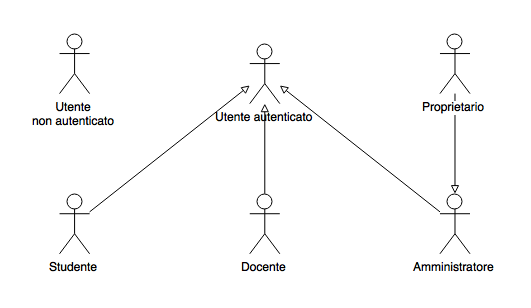
\includegraphics[width=\textwidth]{../img/diagramUCActors.png}
    \caption{Diagramma attori}
\end{figure}

Di seguito viene fornita una breve descrizione degli attori utilizzati nei casi d'uso:

\begin{itemize}
    \item \textbf{Utente non autenticato:} utente che non ha ancora effettuato l'accesso ed è quindi limitato
        ad accedere o registrarsi
    \item \textbf{Utente autenticato:} utente che è registrato al servizio ed ha effettuato l'accesso al
        sistema
    \item \textbf{Studente:} utente autenticato con permessi centrati all'esecuzione di
        questionari
    \item \textbf{Docente:} utente autenticato in grado di gestire studenti, classi, argomenti, questionari
        e domande
    \item \textbf{Amministratore:} utente autenticato che gestisce i docenti
    \item \textbf{Proprietario:} amministratore iniziale che è in grado di creare nuovi amministratori
        e cancellarne di esistenti
\end{itemize}

Nei diagrammi seguenti, le generalizzazioni tra attori non vengono specificate perché
appesantiscono troppo l'immagine. Come riferimento è possibile utilizzare il diagramma mostrato in questa
sezione.

\newpage
\section{Casi d'uso}

\subsection{Struttura di un caso d'uso}
I casi d'uso sono creati secondo lo standard UML 2.4 e sono identificati dalla seguente notazione:
\begin{center}
	UC[codice]: [Titolo]
\end{center}
dove il \textbf{codice} è un numero progressivo identificativo di ogni requisito, gerarchico nel  caso di sotto-casi d'uso tramite la notazione \textit{CodiceUCPadre.CodiceSottoUC}. Per ogni caso d'uso deve inoltre essere indicato:
\begin{itemize}
	\item \textbf{Titolo:} breve ma non ambiguo
	\item \textbf{Attori:} principali e secondari coinvolti
	\item \textbf{Precondizione}
	\item \textbf{Flusso principale degli eventi:} descrizione, eventualmente per punti, del main scenario del Caso d'uso
	\item \textbf{Postcondizione}
\end{itemize}

\hypertarget{UC1}{}
\subsection{Caso d'uso UC1: Registrazione}
\begin{figure}[H]
	\centering
	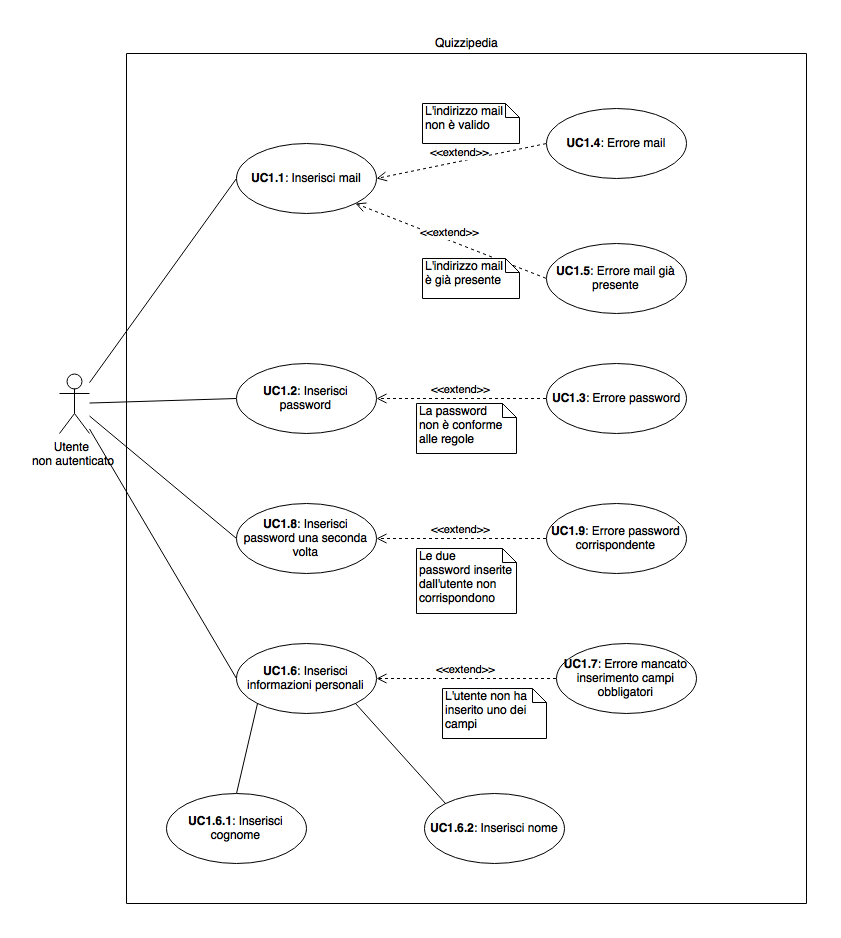
\includegraphics[width=\textwidth]{../img/diagramUC1.png}
	\caption{Caso d'uso UC1: Registrazione}\label{fig:UC1} 
\end{figure}
\begin{itemize}

\item \textbf{Attore}: Utente non autenticato;
\item \textbf{Precondizione}: L’utente non è registrato presso il sistema;

\item \textbf{Flusso principale degli eventi}:
\begin{enumerate}
	\item L'utente inserisce la mail (\hyperlink{UC1.1}{UC1.1});
	\item L'utente inserisce la password (\hyperlink{UC1.2}{UC1.2});
	\item L'utente inserisce la password una seconda volta (\hyperlink{UC1.8}{UC1.8});
	\item L'utente inserisce le proprie infomrazioni personali (\hyperlink{UC1.6}{UC1.6});
	\item L'utente conferma la registrazione;
	
\end{enumerate}
\item \textbf{Postcondizione}: L’utente possiede un’account di tipo studente o docente presso il sistema.
\end{itemize}
\hypertarget{UC1.1}{}
\subsection{Caso d'uso UC1.1: Inserisci mail}

\begin{itemize}

\item \textbf{Attore}: Utente non autenticato; 
\item \textbf{Precondizione}: L'utente non è registrato presso il sistema;

\item \textbf{Flusso principale degli eventi}:
\begin{enumerate}
	\item L'utente inserisce un indirizzo mail valido e non presente nel sistema;
	
\end{enumerate}
\item \textbf{Estensioni}:
\begin{enumerate}
	\item Se l'indirizzo mail non è valido viene visualizzato un errore (\hyperlink{UC1.4}{UC1.4});
	\item Se l'indirizzo mail è già presente nel sistema viene visualizzato un messaggio di errore (\hyperlink{UC1.5}{UC1.5});
	
\end{enumerate}
\item \textbf{Postcondizione}: L'utente ha inserito la mail.
\end{itemize}
\hypertarget{UC1.2}{}
\subsection{Caso d'uso UC1.2: Inserisci password}

\begin{itemize}

\item \textbf{Attore}: Utente non autenticato; 
\item \textbf{Precondizione}: L’utente non è ancora registrato presso il sistema;

\item \textbf{Flusso principale degli eventi}:
\begin{enumerate}
	\item L'utente inserisce una password di almeno 6 caratteri;
	
\end{enumerate}
\item \textbf{Estensioni}:
\begin{enumerate}
	\item Se la password non è conforme alle regole viene visualizzato un messaggio di errore (\hyperlink{UC1.3}{UC1.3});
	
\end{enumerate}
\item \textbf{Postcondizione}: L'utente ha inserito una password.
\end{itemize}
\hypertarget{UC1.3}{}
\subsection{Caso d'uso UC1.3: Errore password}

\begin{itemize}

\item \textbf{Attore}: Utente non autenticato; 
\item \textbf{Precondizione}: Password non conforme alle regole;

\item \textbf{Flusso principale degli eventi}:
\begin{enumerate}
	\item Viene visualizzato un messaggio di errore;
	
\end{enumerate}
\item \textbf{Postcondizione}: L'utente non viene registrato nel sistema.
\end{itemize}
\hypertarget{UC1.4}{}
\subsection{Caso d'uso UC1.4: Errore mail}

\begin{itemize}

\item \textbf{Attore}: Utente non autenticato; 
\item \textbf{Precondizione}: La mail non è un indirizzo valido;

\item \textbf{Flusso principale degli eventi}:
\begin{enumerate}
	\item Viene visualizzato un messaggio di errore;
	
\end{enumerate}
\item \textbf{Postcondizione}: L'utente non viene registrato nel sistema.
\end{itemize}
\hypertarget{UC1.5}{}
\subsection{Caso d'uso UC1.5: Errore mail già presente}

\begin{itemize}

\item \textbf{Attore}: Utente non autenticato; 
\item \textbf{Precondizione}: L'indirizzo mail è già presente nel sistema;

\item \textbf{Flusso principale degli eventi}:
\begin{enumerate}
	\item Viene visualizzato un messaggio di errore;
	
\end{enumerate}
\item \textbf{Postcondizione}: L'utente non viene registrato nel sistema.
\end{itemize}
\hypertarget{UC1.6}{}
\subsection{Caso d'uso UC1.6: Inserisci infomrazioni personali}

\begin{itemize}

\item \textbf{Attore}: Utente non autenticato; 
\item \textbf{Precondizione}: L'utente non è registrato presso il sistema;

\item \textbf{Flusso principale degli eventi}:
\begin{enumerate}
	\item L'utente inserisce il nome (\hyperlink{UC1.6.1}{UC1.6.1});
	\item L'utente inserisce il cognome (\hyperlink{UC1.6.2}{UC1.6.2});
	
\end{enumerate}
\item \textbf{Estensioni}:
\begin{enumerate}
	\item Se l'utente non ha inserito uno dei campi delle informazioni personali viene visualizzato un messaggio di errore (\hyperlink{UC1.7}{UC1.7});
	
\end{enumerate}
\item \textbf{Postcondizione}: L'utente ha inserito le informazioni personali obbligatorie.
\end{itemize}
\hypertarget{UC1.6.1}{}
\subsection{Caso d'uso UC1.6.1: Inserisci nome}

\begin{itemize}

\item \textbf{Attore}: Utente non autenticato; 
\item \textbf{Precondizione}: L’utente non è registrato presso il sistema;

\item \textbf{Flusso principale degli eventi}:
\begin{enumerate}
	\item L'utente inserisce il nome;
	
\end{enumerate}
\item \textbf{Postcondizione}: L'utente ha inserito il nome.
\end{itemize}
\hypertarget{UC1.6.2}{}
\subsection{Caso d'uso UC1.6.2: Inserisci cognome}

\begin{itemize}

\item \textbf{Attore}: Utente non autenticato; 
\item \textbf{Precondizione}: L'utente non è registrato presso il sistema;

\item \textbf{Flusso principale degli eventi}:
\begin{enumerate}
	\item L'utente inserisce il cognome;
	
\end{enumerate}
\item \textbf{Postcondizione}: L'utente ha inserito il cognome.
\end{itemize}
\hypertarget{UC1.7}{}
\subsection{Caso d'uso UC1.7: Errore mancato inserimento campi obbligatori}

\begin{itemize}

\item \textbf{Attore}: Utente non autenticato; 
\item \textbf{Precondizione}: L'utente non ha inserito tutti i campi obbligatori;

\item \textbf{Flusso principale degli eventi}:
\begin{enumerate}
	\item Viene visualizzato un messaggio di errore;
	
\end{enumerate}
\item \textbf{Postcondizione}: L'utente non è registrato presso il sistema.
\end{itemize}
\hypertarget{UC1.8}{}
\subsection{Caso d'uso UC1.8: Secondo inserimento password}

\begin{itemize}

\item \textbf{Attore}: Utente non autenticato; 
\item \textbf{Precondizione}: L’utente non è ancora registrato presso il sistema;

\item \textbf{Flusso principale degli eventi}:
\begin{enumerate}
	\item L'utente inserisce una password uguale a quella già inserita;
	
\end{enumerate}
\item \textbf{Estensioni}:
\begin{enumerate}
	\item Se le due password inserite dall'utente non corrispondono viene visualizzato un messaggio di errore (\hyperlink{UC1.9}{UC1.9});
	
\end{enumerate}
\item \textbf{Postcondizione}: L'utente ha inserito la password una seconda volta.
\end{itemize}
\hypertarget{UC1.9}{}
\subsection{Caso d'uso UC1.9: Errore password non corrispondente}

\begin{itemize}

\item \textbf{Attore}: Utente non autenticato; 
\item \textbf{Precondizione}: Password non uguale a quella già inserita;

\item \textbf{Flusso principale degli eventi}:
\begin{enumerate}
	\item Viene visualizzato un messaggio di errore;
	
\end{enumerate}
\item \textbf{Postcondizione}: L'utente non viene registrato nel sistema.
\end{itemize}
\hypertarget{UC2}{}
\subsection{Caso d'uso UC2: Autenticazione}
\begin{figure}[H]
	\centering
	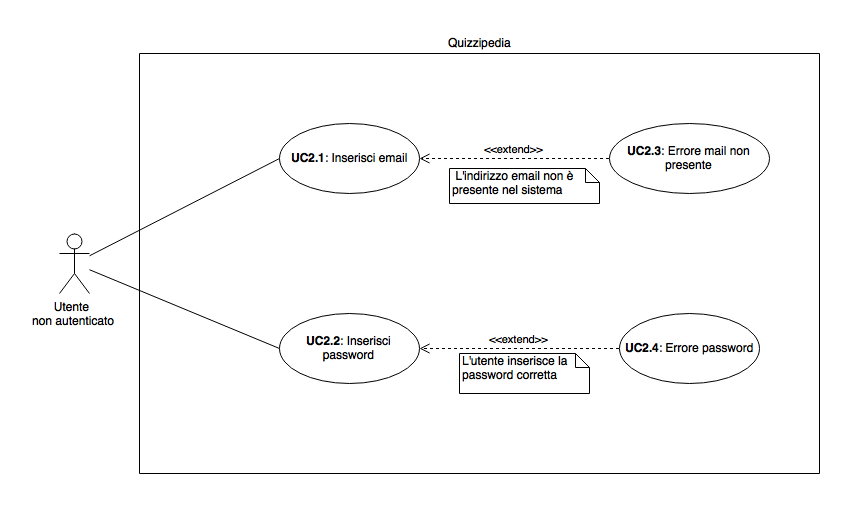
\includegraphics[width=\textwidth]{../img/diagramUC2.png}
	\caption{Caso d'uso UC2: Autenticazione}\label{fig:UC2} 
\end{figure}
\begin{itemize}

\item \textbf{Attore}: Utente non autenticato; 
\item \textbf{Precondizione}: L'utente non è autenticato presso il sistema;

\item \textbf{Flusso principale degli eventi}:
\begin{enumerate}
	\item L'utente inserisce la mail (\hyperlink{UC2.1}{UC2.1});
	\item L'utente inserisce la password (\hyperlink{UC2.2}{UC2.2});
	\item L'utente conferma l'autenticazione;
	
\end{enumerate}
\item \textbf{Postcondizione}: L'utente è autenticato presso il sistema.
\end{itemize}
\hypertarget{UC2.1}{}
\subsection{Caso d'uso UC2.1: Inserisci mail}

\begin{itemize}

\item \textbf{Attore}: Utente non autenticato; 
\item \textbf{Precondizione}: L'utente non è autenticato presso il sistema;

\item \textbf{Flusso principale degli eventi}:
\begin{enumerate}
	\item L'utente inserisce un indirizzo mail presente nel sistema;
	
\end{enumerate}
\item \textbf{Estensioni}:
\begin{enumerate}
	\item Se l'indirizzo email non è presente nel sistema viene visualizzato un messaggio di errore (\hyperlink{UC2.3}{UC2.3});
	
\end{enumerate}
\item \textbf{Postcondizione}: L'utente ha inserito la mail.
\end{itemize}
\hypertarget{UC2.2}{}
\subsection{Caso d'uso UC2.2: Inserisci password}

\begin{itemize}

\item \textbf{Attore}: Utente non autenticato; 
\item \textbf{Precondizione}: L’utente non è ancora autenticato presso il sistema;

\item \textbf{Flusso principale degli eventi}:
\begin{enumerate}
	\item L'utente inserisce la password corretta;
	
\end{enumerate}
\item \textbf{Estensioni}:
\begin{enumerate}
	\item Se la password non corretta viene visualizzato un messaggio di errore (\hyperlink{UC2.4}{UC2.4});
	
\end{enumerate}
\item \textbf{Postcondizione}: L'utente ha inserito una password.
\end{itemize}
\hypertarget{UC2.3}{}
\subsection{Caso d'uso UC2.3: Errore mail non presente}

\begin{itemize}

\item \textbf{Attore}: Utente non autenticato; 
\item \textbf{Precondizione}: L'indirizzo mail non è presente nel sistema;

\item \textbf{Flusso principale degli eventi}:
\begin{enumerate}
	\item Viene visualizzato un messaggio di errore;
	
\end{enumerate}
\item \textbf{Postcondizione}: L'utente non viene autenticato nel sistema.
\end{itemize}
\hypertarget{UC2.4}{}
\subsection{Caso d'uso UC2.4: Errore password}

\begin{itemize}

\item \textbf{Attore}: Utente non autenticato
; 
\item \textbf{Precondizione}: Password non corretta;

\item \textbf{Flusso principale degli eventi}:
\begin{enumerate}
	\item Viene visualizzato un messaggio di errore	;
	
\end{enumerate}
\item \textbf{Postcondizione}: L'utente non viene autenticato nel sistema.
\end{itemize}
\hypertarget{UC3}{}
\subsection{Caso d'uso UC3: Azioni Amministratore}
\begin{figure}[H]
	\centering
	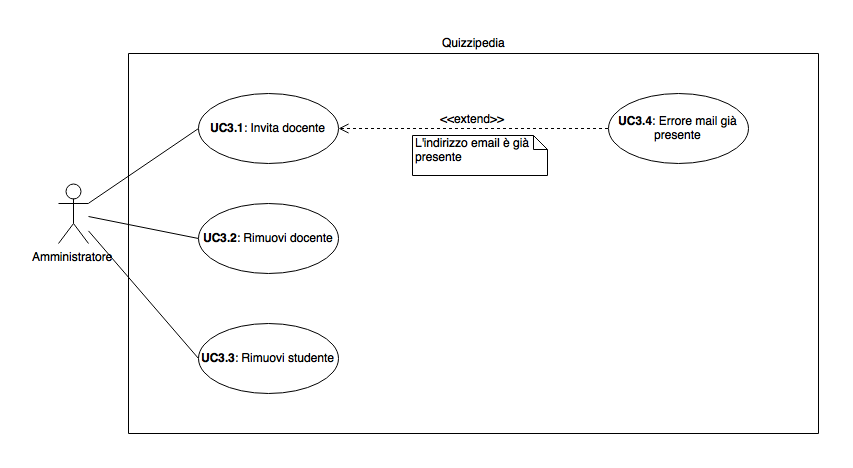
\includegraphics[width=\textwidth]{../img/diagramUC3.png}
	\caption{Caso d'uso UC3: Azioni Amministratore}\label{fig:UC3} 
\end{figure}
\begin{itemize}

\item \textbf{Attore}: Amministratore; 
\item \textbf{Precondizione}: L'amministratore è autenticato nel sistema;

\item \textbf{Flusso principale degli eventi}:
\begin{enumerate}
	\item Amministratore può  invitare un docente (\hyperlink{UC3.1}{UC3.1});
	\item Amministratore può rimuovere un docente (\hyperlink{UC3.2}{UC3.2});
	\item Amministratore può rimuovere uno studente (\hyperlink{UC3.3}{UC3.3});
	
\end{enumerate}
\item \textbf{Postcondizione}: Il sistema ha ottenuto le informazioni sulle operazioni che
l’amministratore desidera eseguire.
\end{itemize}
\hypertarget{UC3.1}{}
\subsection{Caso d'uso UC3.1: Invita docente}

\begin{itemize}

\item \textbf{Attore}: Amministratore; 
\item \textbf{Precondizione}: Amministratore è a conoscenza dell’email del docente da invitare;

\item \textbf{Flusso principale degli eventi}:
\begin{enumerate}
	\item Amministratore inserisce l'email del docente da invitare nel campo opportuno;
	\item Amministratore invia al sistema l'email del docente da invitare;
	
\end{enumerate}
\item \textbf{Estensioni}:
\begin{enumerate}
	\item Se l'indirizzo email è già presente nel sistema viene visualizzato un messaggio di errore (\hyperlink{UC3.4}{UC3.4});
	
\end{enumerate}
\item \textbf{Postcondizione}: Sistema invia token di registrazione del docente alla medesima email.
\end{itemize}
\hypertarget{UC3.2}{}
\subsection{Caso d'uso UC3.2: Rimuovi  docente}

\begin{itemize}

\item \textbf{Attore}: Amministratore; 
\item \textbf{Precondizione}: Il docente da rimuovere deve essere presente nel sistema;

\item \textbf{Flusso principale degli eventi}:
\begin{enumerate}
	\item Amministratore ricerca il docente da rimuovere;
	\item Amministratore seleziona il docente da rimuovere;
	\item Amministratore conferma la rimozione del docente selezionato;
	
\end{enumerate}
\item \textbf{Postcondizione}: Il medesimo docente è stato rimosso dal sistema.
\end{itemize}
\hypertarget{UC3.3}{}
\subsection{Caso d'uso UC3.3: Rimuovi  studente}

\begin{itemize}

\item \textbf{Attore}: Amministratore; 
\item \textbf{Precondizione}: Lo studente da rimuovere deve essere presente nel sistema;

\item \textbf{Flusso principale degli eventi}:
\begin{enumerate}
	\item Amministratore ricerca lo studente da rimuovere;
	\item Amministratore seleziona lo studente da rimuovere;
	\item Amministratore conferma la rimozione dello studente selezionato;
	
\end{enumerate}
\item \textbf{Postcondizione}: Il medesimo studente è stato rimosso dal sistema.
\end{itemize}
\hypertarget{UC3.4}{}
\subsection{Caso d'uso UC3.4: Errore mail già presente}

\begin{itemize}

\item \textbf{Attore}: Amministratore; 
\item \textbf{Precondizione}: L'indirizzo mail è già presente nel sistema;

\item \textbf{Flusso principale degli eventi}:
\begin{enumerate}
	\item Viene visualizzato un messaggio di errore;
	
\end{enumerate}
\item \textbf{Postcondizione}: Non viene inviato alcun invito al docente.
\end{itemize}
\hypertarget{UC4}{}
\subsection{Caso d'uso UC4: Logout}
\begin{figure}[H]
	\centering
	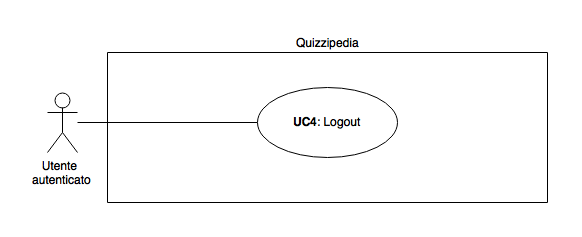
\includegraphics[width=\textwidth]{../img/diagramUC4.png}
	\caption{Caso d'uso UC4: Logout}\label{fig:UC4} 
\end{figure}
\begin{itemize}

\item \textbf{Attore}: Utente autenticato; 
\item \textbf{Precondizione}: L'utente è autenticato nel sistema;

\item \textbf{Flusso principale degli eventi}:
\begin{enumerate}
	\item L'utente seleziona la funzionalità di Logout;
	
\end{enumerate}
\item \textbf{Postcondizione}: L'utente non è più autenticato nel sistema.
\end{itemize}
\hypertarget{UC5}{}
\subsection{Caso d'uso UC5: Gestione classi}
\begin{figure}[H]
	\centering
	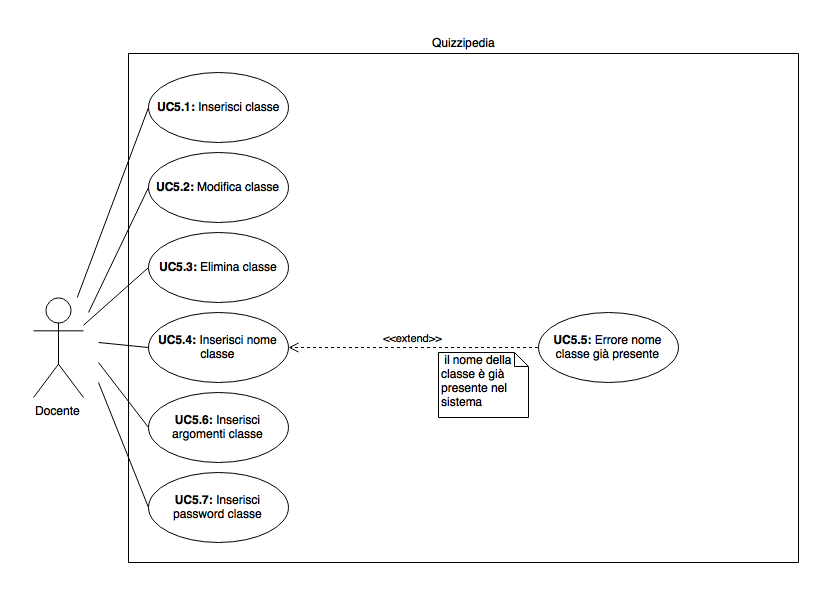
\includegraphics[width=\textwidth]{../img/diagramUC5.png}
	\caption{Caso d'uso UC5: Gestione classi}\label{fig:UC5} 
\end{figure}
\begin{itemize}

\item \textbf{Attore}: Docente; 
\item \textbf{Precondizione}: Il docente è autenticato nel sistema;

\item \textbf{Flusso principale degli eventi}:
\begin{enumerate}
	\item Il docente può creare una nuova classe (\hyperlink{UC5.1}{UC5.1});
	\item Il docente può modificare una classe (\hyperlink{UC5.2}{UC5.2});
	\item Il docente può eliminare una classe (\hyperlink{UC5.3}{UC5.3});
	
\end{enumerate}
\item \textbf{Postcondizione}: Il sistema ha ottenuto le informazioni sulle operazioni che il docente desidera eseguire sulla classe.
\end{itemize}
\hypertarget{UC5.1}{}
\subsection{Caso d'uso UC5.1: Inserisci classe}

\begin{itemize}

\item \textbf{Attore}: Docente; 
\item \textbf{Precondizione}: Il docente è autenticato nel sistema;

\item \textbf{Flusso principale degli eventi}:
\begin{enumerate}
	\item Viene inserito il nome della classe (\hyperlink{UC5.4}{UC5.4});
	\item Vengono inseriti gli argomenti della classe (\hyperlink{UC5.6}{UC5.6});
	\item Viene inserita la password della classe (\hyperlink{UC5.7}{UC5.7});
	\item Viene confermato l'inserimento della classe;
	
\end{enumerate}
\item \textbf{Postcondizione}: È stato creata una nuova classe.
\end{itemize}
\hypertarget{UC5.2}{}
\subsection{Caso d'uso UC5.2: Modifica classe}

\begin{itemize}

\item \textbf{Attore}: Docente; 
\item \textbf{Precondizione}: Il docente è autenticato nel sistema, è presente nel sistema la classe da modificare;

\item \textbf{Flusso principale degli eventi}:
\begin{enumerate}
	\item Viene selezionata una delle proprie classi da modificare;
	\item Può venire modificato il nome (\hyperlink{UC5.4}{UC5.4});
	\item Possono venire modificati gli argomenti (\hyperlink{UC5.6}{UC5.6});
	\item Può venire modificata la password (\hyperlink{UC5.7}{UC5.7});
	\item Viene confermata la modifica;
	
\end{enumerate}
\item \textbf{Postcondizione}: È stata modificata la classe.
\end{itemize}
\hypertarget{UC5.3}{}
\subsection{Caso d'uso UC5.3: Elimina classe}

\begin{itemize}

\item \textbf{Attore}: Docente; 
\item \textbf{Precondizione}: Il docente è autenticato nel sistema, è presente nel sistema la classe da eliminare;

\item \textbf{Flusso principale degli eventi}:
\begin{enumerate}
	\item Viene sezionata una delle proprie classi;
	\item Viene sezionata la funzionalità elimina;
	\item Viene confermata l'eliminazione;
	
\end{enumerate}
\item \textbf{Postcondizione}: È stata eliminata la classe.
\end{itemize}
\hypertarget{UC5.4}{}
\subsection{Caso d'uso UC5.4: Inserisci nome classe}

\begin{itemize}

\item \textbf{Attore}: Docente; 
\item \textbf{Precondizione}: Il docente ha selezionato la classe;

\item \textbf{Flusso principale degli eventi}:
\begin{enumerate}
	\item Il docente inserisce un nome per la classe non ancora presente nel sistema;
	
\end{enumerate}
\item \textbf{Estensioni}:
\begin{enumerate}
	\item Se il nome della classe è già presente nel sistema viene visualizzato un messaggio di errore (\hyperlink{UC5.5}{UC5.5});
	
\end{enumerate}
\item \textbf{Postcondizione}: Il docente ha inserito il nome della classe.
\end{itemize}
\hypertarget{UC5.5}{}
\subsection{Caso d'uso UC5.5: Errore nome classe già presente}

\begin{itemize}

\item \textbf{Attore}: Docente; 
\item \textbf{Precondizione}: Il nome della classe è già presente nel sistema;

\item \textbf{Flusso principale degli eventi}:
\begin{enumerate}
	\item Viene visualizzato un messaggio di errore;
	
\end{enumerate}
\item \textbf{Postcondizione}: La classe non viene inserita nel sistema.
\end{itemize}
\hypertarget{UC5.6}{}
\subsection{Caso d'uso UC5.6: Inserisci argomenti classe}

\begin{itemize}

\item \textbf{Attore}: Docente; 
\item \textbf{Precondizione}: Il docente ha selezionato una classe;

\item \textbf{Flusso principale degli eventi}:
\begin{enumerate}
	\item Il docente inserisce gli argomenti della classe non ancora presente nel sistema;
	
\end{enumerate}
\item \textbf{Postcondizione}: Il docente ha inserito gli argomenti della classe.
\end{itemize}
\hypertarget{UC5.7}{}
\subsection{Caso d'uso UC5.7: Inserisci password classe}

\begin{itemize}

\item \textbf{Attore}: Docente; 
\item \textbf{Precondizione}: Il docente ha selezionato una classe;

\item \textbf{Flusso principale degli eventi}:
\begin{enumerate}
	\item Il docente inserisce una password che servirà per accedere alla classe che verrà creata;
	
\end{enumerate}
\item \textbf{Postcondizione}: Il docente ha inserito la password per accedere alla classe.
\end{itemize}
\hypertarget{UC6}{}
\subsection{Caso d'uso UC6: Gestione questionari}
\begin{figure}[H]
	\centering
	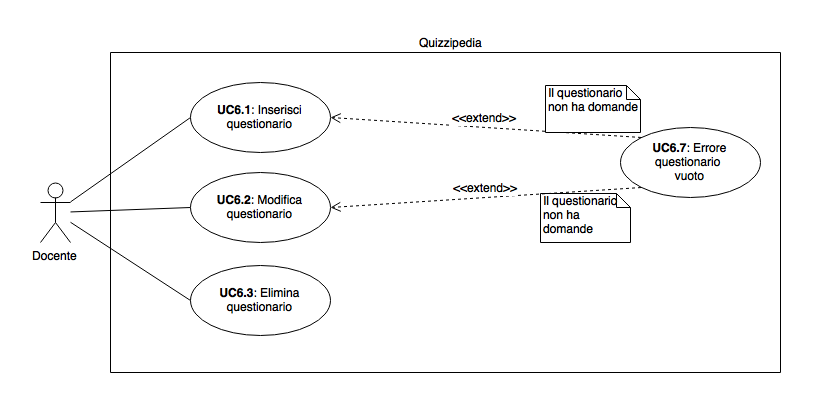
\includegraphics[width=\textwidth]{../img/diagramUC6.png}
	\caption{Caso d'uso UC6: Gestione questionari}\label{fig:UC6} 
\end{figure}
\begin{itemize}

\item \textbf{Attore}: Docente; 
\item \textbf{Precondizione}: Il docente è autenticato nel sistema;

\item \textbf{Flusso principale degli eventi}:
\begin{enumerate}
	\item Il docente può creare un nuovo questionario (\hyperlink{UC6.1}{UC6.1});
	\item Il docente può modificare un questionario (\hyperlink{UC6.2}{UC6.2});
	\item Il docente può eliminare un questionario (\hyperlink{UC6.3}{UC6.3});
	\item Il docente può aggiungere una domanda ad un questionario (\hyperlink{UC6.4}{UC6.4});
	\item Il docente può eliminare una domanda ad un questionario (\hyperlink{UC6.5}{UC6.5});
	
\end{enumerate}
\item \textbf{Postcondizione}: Il sistema ha ottenuto le informazioni sulle operazioni che
il docente desidera eseguire su un questionario.
\end{itemize}
\hypertarget{UC6.1}{}
\subsection{Caso d'uso UC6.1: Inserisci questionario}

\begin{itemize}

\item \textbf{Attore}: Docente; 
\item \textbf{Precondizione}: Il docente è autenticato nel sistema;

\item \textbf{Flusso principale degli eventi}:
\begin{enumerate}
	\item Il docente può aggiungere domande al questionario (\hyperlink{UC6.4}{UC6.4});
	\item Il docente può togliere domande precedentemente aggiunte al questionario (\hyperlink{UC6.5}{UC6.5});
	\item Il docente seleziona gli argomenti del questionario (\hyperlink{UC6.6}{UC6.6});
	\item Il docente conferma la creazione del questionario;
	
\end{enumerate}
\item \textbf{Estensioni}:
\begin{enumerate}
	\item Se il questionario non ha domande viene visualizzato un messaggio d'errore (\hyperlink{UC6.7}{UC6.7});
	
\end{enumerate}
\item \textbf{Postcondizione}: È stato creato un nuovo questionario.
\end{itemize}
\hypertarget{UC6.2}{}
\subsection{Caso d'uso UC6.2: Modifica questionario}

\begin{itemize}

\item \textbf{Attore}: Docente; 
\item \textbf{Precondizione}: Il docente è autenticato nel sistema;

\item \textbf{Flusso principale degli eventi}:
\begin{enumerate}
	\item Ricerca del questionario da modificare (\hyperlink{UC9}{UC9});
	\item Selezione del questionario da modificare;
	\item Il docente può aggiungere domande al questionario (\hyperlink{UC6.4}{UC6.4});
	\item Il docente può togliere domande precedentemente aggiunte al questionario (\hyperlink{UC6.5}{UC6.5});
	\item Il docente può modificare gli argomenti del questionario (\hyperlink{UC6.6}{UC6.6});
	\item Il docente conferma la modifica del questionario;
	
\end{enumerate}
\item \textbf{Postcondizione}: È stato modificato il questionario.
\end{itemize}
\hypertarget{UC6.3}{}
\subsection{Caso d'uso UC6.3: Elimina questionario}

\begin{itemize}

\item \textbf{Attore}: Docente; 
\item \textbf{Precondizione}: Il docente è autenticato nel sistema;

\item \textbf{Flusso principale degli eventi}:
\begin{enumerate}
	\item Ricerca il questionario da eliminare (\hyperlink{UC9}{UC9});
	\item Selezione del questionario da eliminare;
	\item Il docente conferma l'eliminazione;
	
\end{enumerate}
\item \textbf{Postcondizione}: È stato eliminato il questionario.
\end{itemize}
\hypertarget{UC6.4}{}
\subsection{Caso d'uso UC6.4: Aggiungi domanda}

\begin{itemize}

\item \textbf{Attore}: Docente; 
\item \textbf{Precondizione}: È selezionato un questionario dove aggiungere una domanda;

\item \textbf{Flusso principale degli eventi}:
\begin{enumerate}
	\item Viene ricercata un domanda (\hyperlink{UC11}{UC11});
	\item Selezione della domanda;
	\item Conferma inserimento domanda;
	
\end{enumerate}
\item \textbf{Postcondizione}: È stato aggiunta una nuova domanda al questionario selezionato.
\end{itemize}
\hypertarget{UC6.5}{}
\subsection{Caso d'uso UC6.5: Elimina domanda}

\begin{itemize}

\item \textbf{Attore}: Docente; 
\item \textbf{Precondizione}: È stato selezionato un questionario e una domanda da eliminare;

\item \textbf{Flusso principale degli eventi}:
\begin{enumerate}
	\item Viene eliminata la domanda;
	
\end{enumerate}
\item \textbf{Postcondizione}: È stato eliminata la domanda dal questionario selezionato.
\end{itemize}
\hypertarget{UC6.6}{}
\subsection{Caso d'uso UC6.6: Seleziona argomenti questionario}

\begin{itemize}

\item \textbf{Attore}: Docente; 
\item \textbf{Precondizione}: Il docente ha selezionato un questionario;

\item \textbf{Flusso principale degli eventi}:
\begin{enumerate}
	\item Il docente aggiunge un argomento al questionario;
	\item Il docente toglie un argomento al questionario;
	
\end{enumerate}
\item \textbf{Postcondizione}: Il docente ha selezionato gli argomenti del questionario.
\end{itemize}
\hypertarget{UC6.7}{}
\subsection{Caso d'uso UC6.7: Errore questionario vuoto}

\begin{itemize}

\item \textbf{Attore}: Docente; 
\item \textbf{Precondizione}: Il questionario selezionato non ha domande;

\item \textbf{Flusso principale degli eventi}:
\begin{enumerate}
	\item Viene visualizzato un messaggio di errore;
	
\end{enumerate}
\item \textbf{Postcondizione}: Il questionario non viene inserito nel sistema.
\end{itemize}
\hypertarget{UC7}{}
\subsection{Caso d'uso UC7: Gestione domande}
\begin{figure}[H]
	\centering
	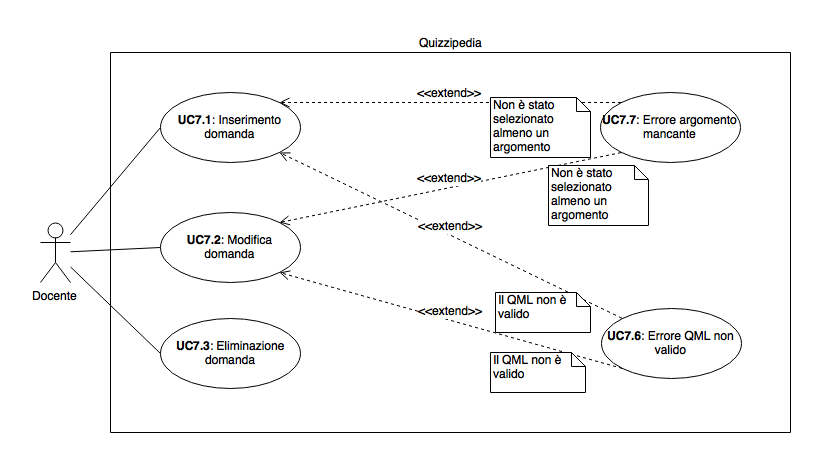
\includegraphics[width=\textwidth]{../img/diagramUC7.png}
	\caption{Caso d'uso UC7: Gestione domande}\label{fig:UC7} 
\end{figure}
\begin{itemize}

\item \textbf{Attore}: Docente; 
\item \textbf{Precondizione}: Il docente è autenticato nel sistema;

\item \textbf{Flusso principale degli eventi}:
\begin{enumerate}
	\item Il docente può creare una nuova domanda (\hyperlink{UC7.1}{UC7.1});
	\item Il docente può modificare una domanda (\hyperlink{UC7.2}{UC7.2});
	\item Il docente può eliminare una domanda (\hyperlink{UC7.3}{UC7.3});
	
\end{enumerate}
\item \textbf{Postcondizione}: Il sistema ha ottenuto le informazioni sulle operazioni che il docente desidera eseguire sulle domande.
\end{itemize}
\hypertarget{UC7.1}{}
\subsection{Caso d'uso UC7.1: Inserimento domanda}

\begin{itemize}

\item \textbf{Attore}: Docente; 
\item \textbf{Precondizione}: Il docente è autenticato nel sistema;

\item \textbf{Flusso principale degli eventi}:
\begin{enumerate}
	\item Il docente seleziona gli argomenti della domanda (\hyperlink{UC7.4}{UC7.4});
	\item Il docente compone la domanda in QML  (\hyperlink{UC7.5}{UC7.5});
	\item Il docente conferma la creazione della domanda;
	
\end{enumerate}
\item \textbf{Postcondizione}: È stata creata una nuova domanda.
\end{itemize}
\hypertarget{UC7.2}{}
\subsection{Caso d'uso UC7.2: Modifica domanda}

\begin{itemize}

\item \textbf{Attore}: Docente; 
\item \textbf{Precondizione}: Il docente è autenticato nel sistema;

\item \textbf{Flusso principale degli eventi}:
\begin{enumerate}
	\item Ricerca della domanda da modificare (\hyperlink{UC11}{UC11});
	\item Selezione della domanda da modificare;
	\item Il docente seleziona gli argomenti della domanda	 (\hyperlink{UC7.4}{UC7.4});
	\item Il docente modifica la domanda in QML	 (\hyperlink{UC7.5}{UC7.5});
	\item Conferma delle modifiche;
	
\end{enumerate}
\item \textbf{Postcondizione}: La domanda è stata modificata.
\end{itemize}
\hypertarget{UC7.3}{}
\subsection{Caso d'uso UC7.3: Elimina domanda}

\begin{itemize}

\item \textbf{Attore}: Docente; 
\item \textbf{Precondizione}: Il docente è autenticato nel sistema;

\item \textbf{Flusso principale degli eventi}:
\begin{enumerate}
	\item Ricerca della domanda da eliminare (\hyperlink{UC11}{UC11});
	\item Selezione della domanda da eliminare;
	\item Conferma per l'eliminazione della domanda	;
	
\end{enumerate}
\item \textbf{Postcondizione}: La domanda è stata eliminata.
\end{itemize}
\hypertarget{UC7.4}{}
\subsection{Caso d'uso UC7.4: Selezione argomenti domanda}

\begin{itemize}

\item \textbf{Attore}: Docente; 
\item \textbf{Precondizione}: Il docente ha selezionato una domanda;

\item \textbf{Flusso principale degli eventi}:
\begin{enumerate}
	\item Il docente aggiunge un argomento alla domanda;
	\item Il docente toglie un argomento alla domanda;
	
\end{enumerate}
\item \textbf{Estensioni}:
\begin{enumerate}
	\item Non è stato selezionato almeno un argomento (\hyperlink{UC7.7}{UC7.7});
	
\end{enumerate}
\item \textbf{Postcondizione}: Il docente ha definito gli argomenti per classificare la domanda
.
\end{itemize}
\hypertarget{UC7.5}{}
\subsection{Caso d'uso UC7.5: Scrittura domanda}

\begin{itemize}

\item \textbf{Attore}: Docente; 
\item \textbf{Precondizione}: Il docente è autenticato presso il sistema;

\item \textbf{Flusso principale degli eventi}:
\begin{enumerate}
	\item Il docente compone la domanda in QML;
	
\end{enumerate}
\item \textbf{Estensioni}:
\begin{enumerate}
	\item Il QML non è valido (\hyperlink{UC7.6}{UC7.6});
	
\end{enumerate}
\item \textbf{Postcondizione}: La domanda è stata scritta in linguaggio QML.
\end{itemize}
\hypertarget{UC7.6}{}
\subsection{Caso d'uso UC7.6: Errore QML non valido}

\begin{itemize}

\item \textbf{Attore}: Docente; 
\item \textbf{Precondizione}: Il QML non è valido;

\item \textbf{Flusso principale degli eventi}:
\begin{enumerate}
	\item Viene visualizzato un messaggio d'errore;
	
\end{enumerate}
\item \textbf{Postcondizione}: Non viene inserita la domanda.
\end{itemize}
\hypertarget{UC7.7}{}
\subsection{Caso d'uso UC7.7: Errore argomento mancante}

\begin{itemize}

\item \textbf{Attore}: Docente; 
\item \textbf{Precondizione}: Non è stato selezionato almeno un argomento;

\item \textbf{Flusso principale degli eventi}:
\begin{enumerate}
	\item Viene visualizzato un messaggio d'errore;
	
\end{enumerate}
\item \textbf{Postcondizione}: Non viene inserita la domanda.
\end{itemize}
\hypertarget{UC8}{}
\subsection{Caso d'uso UC8: Esegui questionario}
\begin{figure}[H]
	\centering
	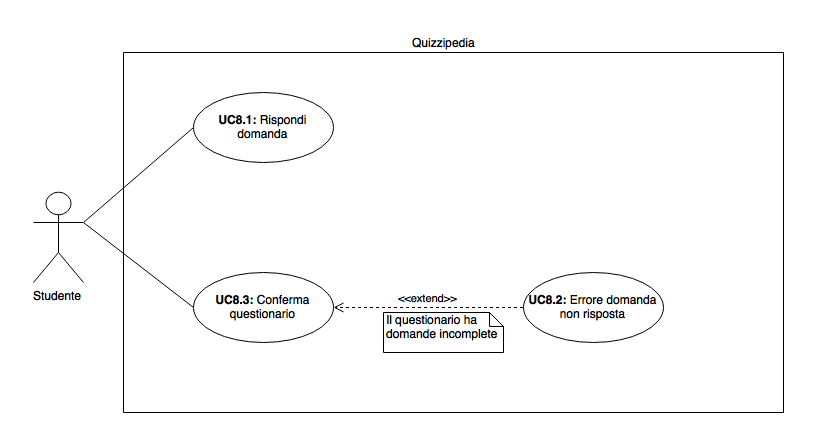
\includegraphics[width=\textwidth]{../img/diagramUC8.png}
	\caption{Caso d'uso UC8: Esegui questionario}\label{fig:UC8} 
\end{figure}
\begin{itemize}

\item \textbf{Attore}: Studente; 
\item \textbf{Precondizione}: Lo studente è autenticato nel sistema;

\item \textbf{Flusso principale degli eventi}:
\begin{enumerate}
	\item Lo studente risponde ad una domanda (\hyperlink{UC8.1}{UC8.1});
	\item Lo studente può andare alla domanda successiva;
	\item Lo studente può andare alla domanda precedente;
	\item Lo studente conferma il questionario (\hyperlink{UC8.3}{UC8.3});
	
\end{enumerate}
\item \textbf{Postcondizione}: Il questionario è stato compilato e vengono visualizzati i risultati.
\end{itemize}
\hypertarget{UC8.1}{}
\subsection{Caso d'uso UC8.1: Rispondi domanda}

\begin{itemize}

\item \textbf{Attore}: Studente; 
\item \textbf{Precondizione}: Lo studente ha iniziato l'esecuzione di un questionario;

\item \textbf{Flusso principale degli eventi}:
\begin{enumerate}
	\item Lo studente seleziona la risposta che ritiene esatta con le modalità previste dal tipo di domanda;
	
\end{enumerate}
\item \textbf{Postcondizione}: Lo studente ha risposto alla domanda.
\end{itemize}
\hypertarget{UC8.2}{}
\subsection{Caso d'uso UC8.2: Errore domanda non risposta}

\begin{itemize}

\item \textbf{Attore}: Studente; 
\item \textbf{Precondizione}: Lo studente non ha riposto ad alcune domande nel momento in cui conferma il questionario;

\item \textbf{Flusso principale degli eventi}:
\begin{enumerate}
	\item Viene visualizzato un messaggio di errore;
	
\end{enumerate}
\item \textbf{Postcondizione}: Il questionario non viene terminato.
\end{itemize}
\hypertarget{UC8.3}{}
\subsection{Caso d'uso UC8.3: Conferma  questionario}

\begin{itemize}

\item \textbf{Attore}: Studente; 
\item \textbf{Precondizione}: Lo studente è autenticato nel sistema;

\item \textbf{Flusso principale degli eventi}:
\begin{enumerate}
	\item Lo studente conferma il questionario;
	
\end{enumerate}
\item \textbf{Estensioni}:
\begin{enumerate}
	\item Se quando lo studente conferma il questionario ci sono domande non risposte viene visualizzato un errore (\hyperlink{UC8.2}{UC8.2});
	
\end{enumerate}
\item \textbf{Postcondizione}: Il questionario viene confermato.
\end{itemize}
\hypertarget{UC9}{}
\subsection{Caso d'uso UC9: Ricerca questionario}
\begin{figure}[H]
	\centering
	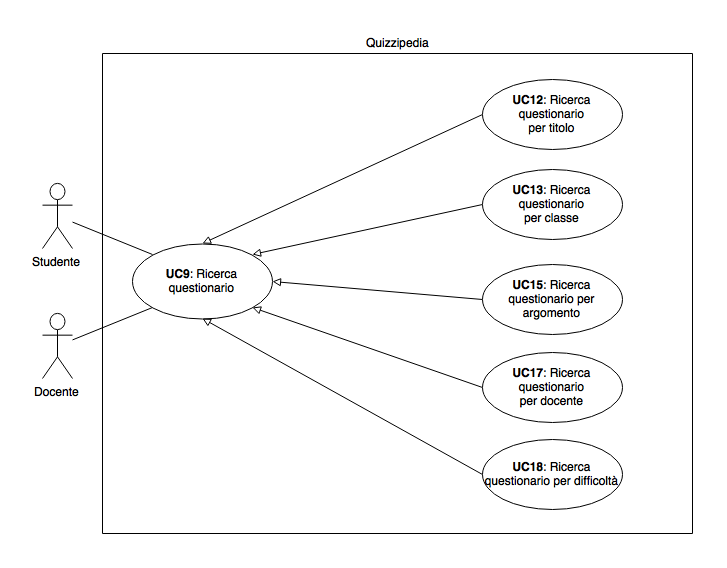
\includegraphics[width=\textwidth]{../img/diagramUC9.png}
	\caption{Caso d'uso UC9: Ricerca questionario}\label{fig:UC9} 
\end{figure}
\begin{itemize}

\item \textbf{Attore}: Studente, Docente; 
\item \textbf{Precondizione}: L'utente è autenticato presso il sistema;

\item \textbf{Flusso principale degli eventi}:
\begin{enumerate}
	\item L'utente inserisce i dati per la ricerca;
	
\end{enumerate}
\item \textbf{Postcondizione}: Il sistema mostra la lista dei questionari che soddisfano la ricerca.
\end{itemize}
\hypertarget{UC10}{}
\subsection{Caso d'uso UC10: Gestione account}
\begin{figure}[H]
    \centering
	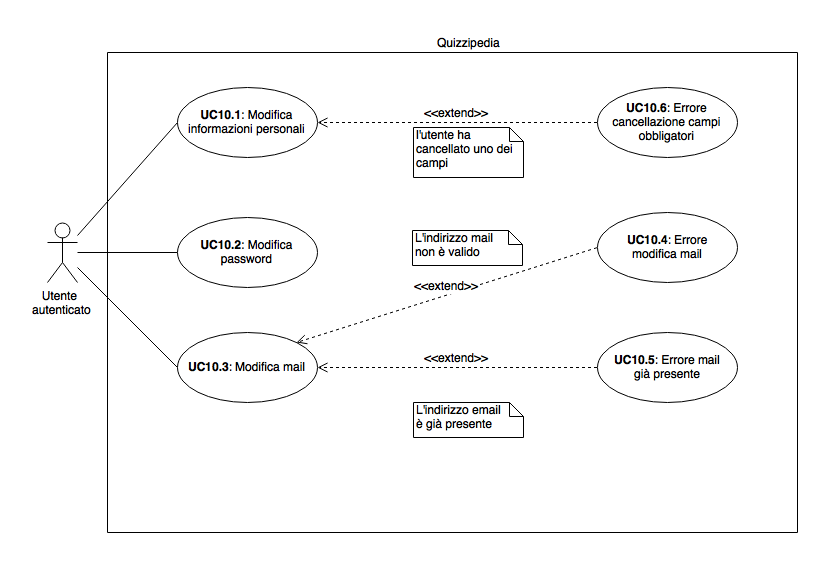
\includegraphics[width=\textwidth]{../img/diagramUC10.png}
	\caption{Caso d'uso UC10: Gestione account}\label{fig:UC10} 
\end{figure}
\begin{itemize}

\item \textbf{Attore}: Utente autenticato; 
\item \textbf{Precondizione}: L'utente è autenticato nel sistema;

\item \textbf{Flusso principale degli eventi}:
\begin{enumerate}
	\item L’utente visualizza la propria mail, nome e cognome;
	\item L’utente modifica le proprie informazioni personali (\hyperlink{UC10.1}{UC10.1});
	\item L’utente modifica la propria mail (\hyperlink{UC10.3}{UC10.3});
	\item L’utente modifica la propria password (\hyperlink{UC10.2}{UC10.2});
	\item L'utente conferma le modifiche effettuate;
	
\end{enumerate}
\item \textbf{Postcondizione}: Il sistema ha apportato le modifiche all'account dell'utente.
\end{itemize}
\hypertarget{UC10.1}{}
\subsection{Caso d'uso UC10.1: Modifica informazioni personali}

\begin{itemize}

\item \textbf{Attore}: Utente autenticato; 
\item \textbf{Precondizione}: L'utente è autenticato nel sistema;

\item \textbf{Flusso principale degli eventi}:
\begin{enumerate}
	\item L’utente modifica il proprio nome (\hyperlink{UC10.1.1}{UC10.1.1});
	\item L’utente modifica il proprio congome (\hyperlink{UC10.1.2}{UC10.1.2});
	
\end{enumerate}
\item \textbf{Estensioni}:
\begin{enumerate}
	\item Se l'utente ha cancellato uno dei campi delle informazioni personali viene visualizzato un messaggio di errore (\hyperlink{UC10.6}{UC10.6});
	
\end{enumerate}
\item \textbf{Postcondizione}: L'utente ha modificato le proprie informazioni personali.
\end{itemize}
\hypertarget{UC10.1.1}{}
\subsection{Caso d'uso UC10.1.1: Modifica nome}

\begin{itemize}

\item \textbf{Attore}: Utente autenticato; 
\item \textbf{Precondizione}: L'utente è autenticato nel sistema;

\item \textbf{Flusso principale degli eventi}:
\begin{enumerate}
	\item L'utente modifica il nome;
	
\end{enumerate}
\item \textbf{Postcondizione}: L'utente ha modificato il nome.
\end{itemize}
\hypertarget{UC10.1.2}{}
\subsection{Caso d'uso UC10.1.2: Modifica cognome}

\begin{itemize}

\item \textbf{Attore}: Utente autenticato; 
\item \textbf{Precondizione}: L'utente è autenticato nel sistema;

\item \textbf{Flusso principale degli eventi}:
\begin{enumerate}
	\item L'utente modifica il cognome;
	
\end{enumerate}
\item \textbf{Postcondizione}: L'utente ha modificato il cognome.
\end{itemize}
\hypertarget{UC10.2}{}
\subsection{Caso d'uso UC10.2: Modifica password}

\begin{itemize}
\item \textbf{Attore}: Utente autenticato; 
\item \textbf{Precondizione}: L’utente ha richiesto di modificare la propria password;

\item \textbf{Flusso principale degli eventi}:
\begin{enumerate}
	\item L’utente inserisce l’attuale password in uso (\hyperlink{UC10.2.1}{UC10.2.1});
	\item L’utente inserisce la nuova password (\hyperlink{UC10.2.2}{UC10.2.2});
	\item L’utente inserisce la password nuova una seconda volta (\hyperlink{UC10.2.3}{UC10.2.3});
	
\end{enumerate}
\item \textbf{Postcondizione}: L'utente ha inserito la nuova password correttamente.
\end{itemize}
\hypertarget{UC10.2.1}{}
\subsection{Caso d'uso UC10.2.1:  Inserimento vecchia password}

\begin{itemize}

\item \textbf{Attore}: Utente autenticato; 
\item \textbf{Precondizione}: Il sistema ha visualizzato la sezione dove poter inserire l’attuale password che andrà cambiata;

\item \textbf{Flusso principale degli eventi}:
\begin{enumerate}
	\item L'utente inserisce la password in uso;
	
\end{enumerate}
\item \textbf{Estensioni}:
\begin{enumerate}
	\item Se la password non è corretta viene visualizzato un messaggio di errore (\hyperlink{UC10.2.4}{UC10.2.4});
	
\end{enumerate}
\item \textbf{Postcondizione}: Il sistema convalida la password appena inserita.
\end{itemize}
\hypertarget{UC10.2.2}{}
\subsection{Caso d'uso UC10.2.2:  Inserimento nuova password}

\begin{itemize}

\item \textbf{Attore}: Utente autenticato; 
\item \textbf{Precondizione}: Il sistema ha visualizzato la sezione dove poter inserire la nuova password;

\item \textbf{Flusso principale degli eventi}:
\begin{enumerate}
	\item L'utente inserisce una password di almeno 6 caratteri;
	
\end{enumerate}
\item \textbf{Estensioni}:
\begin{enumerate}
	\item Se la password non è conforme alle regole viene visualizzato un messaggio di errore (\hyperlink{UC10.2.5}{UC10.2.5});
	
\end{enumerate}
\item \textbf{Postcondizione}: Il sistema convalida la nuova password appena inserita.
\end{itemize}
\hypertarget{UC10.2.3}{}
\subsection{Caso d'uso UC10.2.3: Conferma nuova password}

\begin{itemize}

\item \textbf{Attore}: Utente autenticato; 
\item \textbf{Precondizione}: Il sistema ha visualizzato la sezione dove inserire la conferma della nuova password;

\item \textbf{Flusso principale degli eventi}:
\begin{enumerate}
	\item L'utente inserisce una password uguale a quella già inserita;
	
\end{enumerate}
\item \textbf{Estensioni}:
\begin{enumerate}
	\item Se le due password inerite dall'utente non corrispondono viene visualizzato un messaggio di errore (\hyperlink{UC10.2.6}{UC10.2.6});
	
\end{enumerate}
\item \textbf{Postcondizione}: Il sistema convalida la conferma della nuova password appena inserita.
\end{itemize}
\hypertarget{UC10.2.4}{}
\subsection{Caso d'uso UC10.2.4: Errore password}

\begin{itemize}

\item \textbf{Attore}: Utente autenticato; 
\item \textbf{Precondizione}: Password non corretta;

\item \textbf{Flusso principale degli eventi}:
\begin{enumerate}
	\item Viene visualizzato un messaggio di errore;
	
\end{enumerate}
\item \textbf{Postcondizione}: La password non viene modificata.
\end{itemize}
\hypertarget{UC10.2.5}{}
\subsection{Caso d'uso UC10.2.5: Errore password}

\begin{itemize}

\item \textbf{Attore}: Utente autenticato; 
\item \textbf{Precondizione}: Password non conforme alle regole;

\item \textbf{Flusso principale degli eventi}:
\begin{enumerate}
	\item Viene visualizzato un messaggio di errore;
	
\end{enumerate}
\item \textbf{Postcondizione}: La password non viene modificata.
\end{itemize}
\hypertarget{UC10.2.6}{}
\subsection{Caso d'uso UC10.2.6: Errore password non corrispondente}

\begin{itemize}

\item \textbf{Attore}: Utente autenticato; 
\item \textbf{Precondizione}: Password non uguale a quella già inserita;

\item \textbf{Flusso principale degli eventi}:
\begin{enumerate}
	\item Viene visualizzato un messaggio di errore;
	
\end{enumerate}
\item \textbf{Postcondizione}: La password dell'utente non viene modificata.
\end{itemize}
\hypertarget{UC10.3}{}
\subsection{Caso d'uso UC10.3: Modifica mail}

\begin{itemize}

\item \textbf{Attore}: Utente autenticato; 
\item \textbf{Precondizione}: L'utente è autenticato nel sistema;

\item \textbf{Flusso principale degli eventi}:
\begin{enumerate}
	\item L'utente inserisce un indirizzo mail valido e non presente nel sistema;
	
\end{enumerate}
\item \textbf{Estensioni}:
\begin{enumerate}
	\item Se l'indirizzo mail non è valido viene visualizzato un errore (\hyperlink{UC10.4}{UC10.4});
	\item Se l'indirizzo email è già presente nel sistema viene visualizzato un messaggio di errore (\hyperlink{UC10.5}{UC10.5});
	
\end{enumerate}
\item \textbf{Postcondizione}: L'utente ha modificato la propria mail.
\end{itemize}
\hypertarget{UC10.4}{}
\subsection{Caso d'uso UC10.4: Errore modifica mail}

\begin{itemize}

\item \textbf{Attore}: Utente autenticato; 
\item \textbf{Precondizione}: La mail non è un indirizzo valido;

\item \textbf{Flusso principale degli eventi}:
\begin{enumerate}
	\item Viene visualizzato un messaggio di errore;
	
\end{enumerate}
\item \textbf{Postcondizione}: La mail non viene modificata.
\end{itemize}
\hypertarget{UC10.5}{}
\subsection{Caso d'uso UC10.5: Errore mail già presente}

\begin{itemize}

\item \textbf{Attore}: Utente autenticato; 
\item \textbf{Precondizione}: L'indirizzo mail è già presente nel sistema;

\item \textbf{Flusso principale degli eventi}:
\begin{enumerate}
	\item Viene visualizzato un messaggio di errore;
	
\end{enumerate}
\item \textbf{Postcondizione}: La mail non viene modificata.
\end{itemize}
\hypertarget{UC10.6}{}
\subsection{Caso d'uso UC10.6: Errore cancellazione campi obbligatori}

\begin{itemize}

\item \textbf{Attore}: Utente autenticato; 
\item \textbf{Precondizione}: L'utente non ha inserito tutti i campi;

\item \textbf{Flusso principale degli eventi}:
\begin{enumerate}
	\item Viene visualizzato un messaggio di errore;
	
\end{enumerate}
\item \textbf{Postcondizione}: Non viene effettuata la modifica.
\end{itemize}
\hypertarget{UC11}{}
\subsection{Caso d'uso UC11: Ricerca domanda}
\begin{figure}[H]
	\centering
	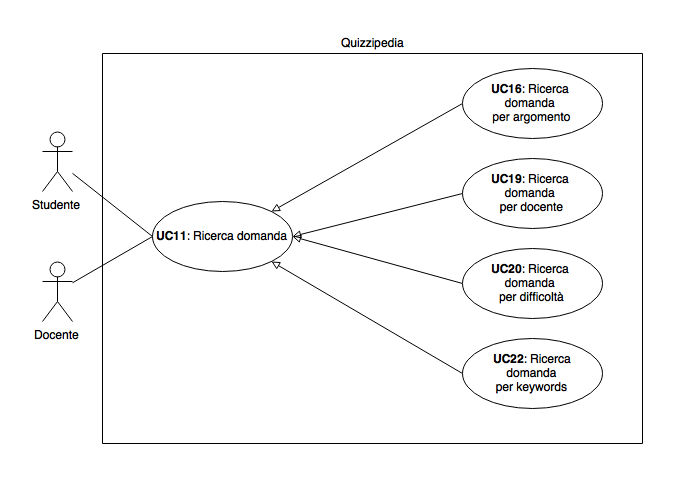
\includegraphics[width=\textwidth]{../img/diagramUC11.png}
	\caption{Caso d'uso UC11: Ricerca domanda}\label{fig:UC11} 
\end{figure}
\begin{itemize}

\item \textbf{Attore}: Studente, Docente; 
\item \textbf{Precondizione}: L'utente è autenticato presso il sistema;

\item \textbf{Flusso principale degli eventi}:
\begin{enumerate}
	\item L'utente inserisce i dati per la ricerca	;
	
\end{enumerate}
\item \textbf{Postcondizione}: Il sistema mostra la lista delle domande che soddisfano la ricerca.
\end{itemize}
\hypertarget{UC12}{}
\subsection{Caso d'uso UC12: Ricerca questionario per titolo}

\begin{itemize}

\item \textbf{Attore}: Studente, Docente; 
\item \textbf{Precondizione}: L'utente è autenticato presso il sistema;

\item \textbf{Flusso principale degli eventi}:
\begin{enumerate}
	\item L'utente inserisce i dati per la ricerca;
	
\end{enumerate}
\item \textbf{Postcondizione}: Il sistema mostra la lista dei questionari che soddisfano la ricerca.
\end{itemize}
\hypertarget{UC13}{}
\subsection{Caso d'uso UC13: Ricerca questionario per classe}

\begin{itemize}

\item \textbf{Attore}: Studente, Docente; 
\item \textbf{Precondizione}: L'utente è autenticato presso il sistema;

\item \textbf{Flusso principale degli eventi}:
\begin{enumerate}
	\item L'utente inserisce i dati per la ricerca;
	
\end{enumerate}
\item \textbf{Postcondizione}: Il sistema mostra la lista dei questionari che soddisfano la ricerca.
\end{itemize}
\hypertarget{UC14}{}
\subsection{Caso d'uso UC14: Ricerca classe}
\begin{figure}[H]
	\centering
	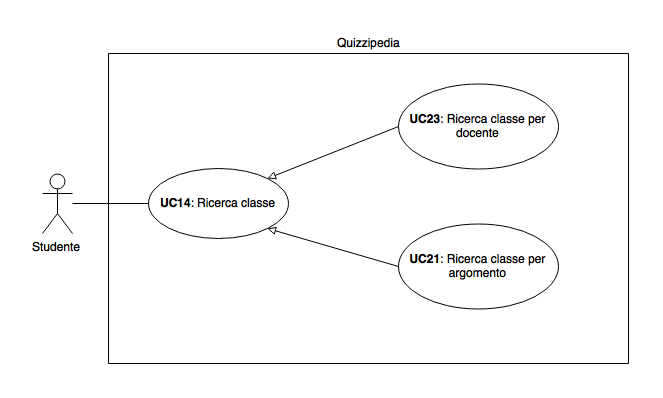
\includegraphics[width=\textwidth]{../img/diagramUC14.png}
	\caption{Caso d'uso UC14: Ricerca classe}\label{fig:UC14} 
\end{figure}
\begin{itemize}

\item \textbf{Attore}: Studente; 
\item \textbf{Precondizione}: Lo studente è autenticato presso il sistema;

\item \textbf{Flusso principale degli eventi}:
\begin{enumerate}
	\item Lo studente inserisce i dati per la ricerca;
	
\end{enumerate}
\item \textbf{Postcondizione}: Il sistema mostra la lista delle classi che soddisfano la ricerca.
\end{itemize}
\hypertarget{UC15}{}
\subsection{Caso d'uso UC15: Ricerca questionario per argomento}

\begin{itemize}

\item \textbf{Attore}: Studente, Docente; 
\item \textbf{Precondizione}: L'utente è autenticato presso il sistema;

\item \textbf{Flusso principale degli eventi}:
\begin{enumerate}
	\item L'utente inserisce i dati per la ricerca;
	
\end{enumerate}
\item \textbf{Postcondizione}: Il sistema mostra la lista dei questionari che soddisfano la ricerca.
\end{itemize}
\hypertarget{UC16}{}
\subsection{Caso d'uso UC16: Ricerca domanda per argomento}

\begin{itemize}

\item \textbf{Attore}: Studente, Docente
; 
\item \textbf{Precondizione}: L'utente è autenticato presso il sistema
;

\item \textbf{Flusso principale degli eventi}:
\begin{enumerate}
	\item L'utente inserisce i dati per la ricerca	;
	
\end{enumerate}
\item \textbf{Postcondizione}: Il sistema mostra la lista delle domande che soddisfano la ricerca
.
\end{itemize}
\hypertarget{UC17}{}
\subsection{Caso d'uso UC17: Ricerca questionario per docente}

\begin{itemize}

\item \textbf{Attore}: Studente, Docente; 
\item \textbf{Precondizione}: L'utente è autenticato presso il sistema;

\item \textbf{Flusso principale degli eventi}:
\begin{enumerate}
	\item L'utente inserisce i dati per la ricerca;
	
\end{enumerate}
\item \textbf{Postcondizione}: Il sistema mostra la lista dei questionari che soddisfano la ricerca.
\end{itemize}
\hypertarget{UC18}{}
\subsection{Caso d'uso UC18: Ricerca questionario per difficoltà}

\begin{itemize}

\item \textbf{Attore}: Studente, Docente; 
\item \textbf{Precondizione}: L'utente è autenticato presso il sistema;

\item \textbf{Flusso principale degli eventi}:
\begin{enumerate}
	\item L'utente inserisce i dati per la ricerca;
	
\end{enumerate}
\item \textbf{Postcondizione}: Il sistema mostra la lista dei questionari che soddisfano la ricerca.
\end{itemize}
\hypertarget{UC19}{}
\subsection{Caso d'uso UC19: Ricerca domanda per docente}

\begin{itemize}

\item \textbf{Attore}: Studente, Docente
; 
\item \textbf{Precondizione}: L'utente è autenticato presso il sistema
;

\item \textbf{Flusso principale degli eventi}:
\begin{enumerate}
	\item L'utente inserisce i dati per la ricerca	;
	
\end{enumerate}
\item \textbf{Postcondizione}: Il sistema mostra la lista delle domande che soddisfano la ricerca
.
\end{itemize}
\hypertarget{UC20}{}
\subsection{Caso d'uso UC20: Ricerca domanda per difficoltà}

\begin{itemize}

\item \textbf{Attore}: Studente, Docente
; 
\item \textbf{Precondizione}: L'utente è autenticato presso il sistema
;

\item \textbf{Flusso principale degli eventi}:
\begin{enumerate}
	\item L'utente inserisce i dati per la ricerca	;
	
\end{enumerate}
\item \textbf{Postcondizione}: Il sistema mostra la lista delle domande che soddisfano la ricerca
.
\end{itemize}
\hypertarget{UC21}{}
\subsection{Caso d'uso UC21: Ricerca classe per argomento}

\begin{itemize}

\item \textbf{Attore}: Studente; 
\item \textbf{Precondizione}: Lo studente è autenticato presso il sistema;

\item \textbf{Flusso principale degli eventi}:
\begin{enumerate}
	\item Lo studente inserisce i dati per la ricerca;
	
\end{enumerate}
\item \textbf{Postcondizione}: Il sistema mostra la lista delle classi che soddisfano la ricerca.
\end{itemize}
\hypertarget{UC22}{}
\subsection{Caso d'uso UC22: Ricerca domanda per keywords}

\begin{itemize}

\item \textbf{Attore}: Studente, Docente
; 
\item \textbf{Precondizione}: L'utente è autenticato presso il sistema
;

\item \textbf{Flusso principale degli eventi}:
\begin{enumerate}
	\item L'utente inserisce i dati per la ricerca	;
	
\end{enumerate}
\item \textbf{Postcondizione}: Il sistema mostra la lista delle domande che soddisfano la ricerca
.
\end{itemize}
\hypertarget{UC23}{}
\subsection{Caso d'uso UC23: Ricerca classe per docente}

\begin{itemize}

\item \textbf{Attore}: Studente; 
\item \textbf{Precondizione}: Lo studente è autenticato presso il sistema;

\item \textbf{Flusso principale degli eventi}:
\begin{enumerate}
	\item Lo studente inserisce i dati per la ricerca;
	
\end{enumerate}
\item \textbf{Postcondizione}: Il sistema mostra la lista delle classi che soddisfano la ricerca.
\end{itemize}
\hypertarget{UC24}{}
\subsection{Caso d'uso UC24: Iscrizione ad una classe}
\begin{figure}[H]
	\centering
	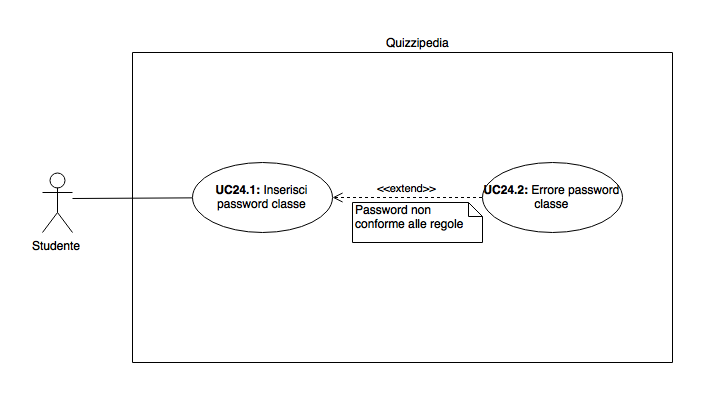
\includegraphics[width=\textwidth]{../img/diagramUC24.png}
	\caption{Caso d'uso UC24: Iscrizione ad una classe}\label{fig:UC24} 
\end{figure}
\begin{itemize}

\item \textbf{Attore}: Studente; 
\item \textbf{Precondizione}: Lo studente è autenticato presso il sistema;

\item \textbf{Flusso principale degli eventi}:
\begin{enumerate}
	\item Lo studente cerca una classe (\hyperlink{UC14}{UC14});
	\item Lo studente inserisce la password per iscriversi alla classe (\hyperlink{UC24.1}{UC24.1});
	\item Lo studente conferma l'iscrizione alla classe;
	
\end{enumerate}
\item \textbf{Postcondizione}: Lo studente si è iscritto alla classe desiderata.
\end{itemize}
\hypertarget{UC24.1}{}
\subsection{Caso d'uso UC24.1: Inserisci password classe}

\begin{itemize}

\item \textbf{Attore}: Studente; 
\item \textbf{Precondizione}: Lo studente è autenticato presso il sistema;

\item \textbf{Flusso principale degli eventi}:
\begin{enumerate}
	\item Lo studente inserisce la password corretta per iscriversi alla classe;
	
\end{enumerate}
\item \textbf{Estensioni}:
\begin{enumerate}
	\item Se la password inserita non è corretta viene visualizzato un messaggio di errore (\hyperlink{UC24.2}{UC24.2});
	
\end{enumerate}
\item \textbf{Postcondizione}: Lo studente ha inserito la password per iscriversi alla classe.
\end{itemize}
\hypertarget{UC24.2}{}
\subsection{Caso d'uso UC24.2: Errore password classe}

\begin{itemize}

\item \textbf{Attore}: Studente; 
\item \textbf{Precondizione}: Lo studente ha inserito una password errata per iscriversi alla classe;

\item \textbf{Flusso principale degli eventi}:
\begin{enumerate}
	\item Viene visualizzato un messaggio di errore;
	
\end{enumerate}
\item \textbf{Postcondizione}: Lo studente non viene iscritto alla classe.
\end{itemize}
\hypertarget{UC25}{}
\subsection{Caso d'uso UC25: Azioni proprietario}
\begin{figure}[H]
	\centering
	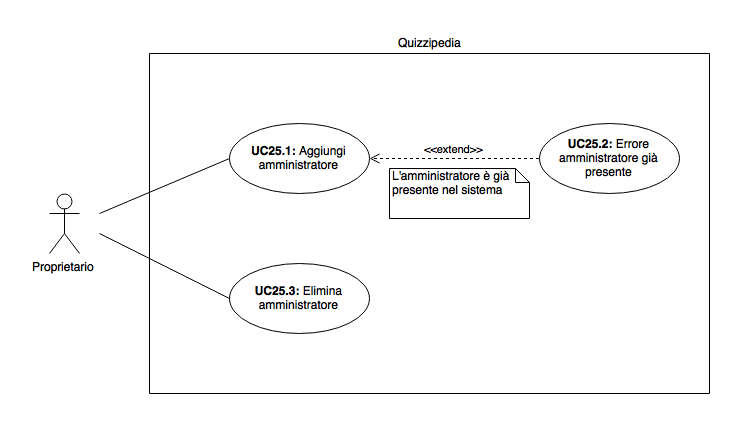
\includegraphics[width=\textwidth]{../img/diagramUC25.png}
	\caption{Caso d'uso UC25: Azioni proprietario}\label{fig:UC25} 
\end{figure}
\begin{itemize}

\item \textbf{Attore}: Proprietario; 
\item \textbf{Precondizione}: Il proprietario è autenticato presso il sistema;

\item \textbf{Flusso principale degli eventi}:
\begin{enumerate}
	\item Il proprietario può aggiungere un nuovo amministratore (\hyperlink{UC25.1}{UC25.1});
	\item Il proprietario può rimuovere un nuovo amministratore (\hyperlink{UC25.3}{UC25.3});
	
\end{enumerate}
\item \textbf{Postcondizione}: Il sistema ha ottenuto le informazioni sulle operazioni che il proprietario desidera eseguire.
\end{itemize}
\hypertarget{UC25.1}{}
\subsection{Caso d'uso UC25.1: Aggiungi amministratore}

\begin{itemize}

\item \textbf{Attore}: Proprietario; 
\item \textbf{Precondizione}: Il proprietario è autenticato nel sistema;

\item \textbf{Flusso principale degli eventi}:
\begin{enumerate}
	\item L'amministratore inserisce mail del nuovo amministratore;
	\item L'amministratore seleziona la funzionalità di aggiunta amministratore;
	
\end{enumerate}
\item \textbf{Estensioni}:
\begin{enumerate}
	\item Se l’amministratore inserisce una mail già censita dal sistema viene visualizzato un errore (\hyperlink{UC25.2}{UC25.2});
	
\end{enumerate}
\item \textbf{Postcondizione}: È stato inserito un nuovo account amministratore.
\end{itemize}
\hypertarget{UC25.2}{}
\subsection{Caso d'uso UC25.2: Errore amministratore già presente}

\begin{itemize}

\item \textbf{Attore}: Proprietario; 
\item \textbf{Precondizione}: L'indirizzo mail dell'amministratore è già presente nel sistema;

\item \textbf{Flusso principale degli eventi}:
\begin{enumerate}
	\item Viene visualizzato un messaggio di errore;
	
\end{enumerate}
\item \textbf{Postcondizione}: Il nuovo amministratore non viene registrato nel sistema.
\end{itemize}
\hypertarget{UC25.3}{}
\subsection{Caso d'uso UC25.3: Elimina amministratore}

\begin{itemize}

\item \textbf{Attore}: Propietario; 
\item \textbf{Precondizione}: Il proprietario è autenticato nel sistema;

\item \textbf{Flusso principale degli eventi}:
\begin{enumerate}
	\item Il proprietario seleziona l'account amministratore da eliminare;
	\item Il proprietario seleziona la funzionalità di eliminazione amministratore;
	\item Il proprietario conferma l'eliminazione dell'amministratore;
	
\end{enumerate}
\item \textbf{Postcondizione}: È stato eliminato un amministratore.
\end{itemize}
\hypertarget{UC26}{}
\subsection{Caso d'uso UC26: Visualizza statistiche}
\begin{figure}[H]
    \centering
	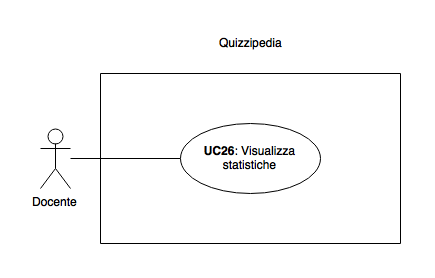
\includegraphics[width=\textwidth]{../img/diagramUC26.png}
	\caption{Caso d'uso UC26: Visualizza statistiche}\label{fig:UC26} 
\end{figure}
\begin{itemize}

\item \textbf{Attore}: Docente; 
\item \textbf{Precondizione}: Il docente è autenticato presso il sistema;

\item \textbf{Flusso principale degli eventi}:
\begin{enumerate}
	\item Il docente può visualizzare le statistiche;
	
\end{enumerate}
\item \textbf{Postcondizione}: Il docente ha visualizzato le statistiche a cui era interessato.
\end{itemize}
\hypertarget{UC27}{}
\subsection{Caso d'uso UC27: Statistiche domanda}

\begin{itemize}

\item \textbf{Attore}: Docente; 
\item \textbf{Precondizione}: Il docente è autenticato presso il sistema;

\item \textbf{Flusso principale degli eventi}:
\begin{enumerate}
	\item Il docente ricerca una domanda (\hyperlink{UC11}{UC11});
	\item Il docente seleziona la domanda interessata;
	
\end{enumerate}
\item \textbf{Postcondizione}: Il docente ha visualizzato le statistiche relative alla domanda a cui era interessato.
\end{itemize}
\hypertarget{UC28}{}
\subsection{Caso d'uso UC28: Statistiche questionario}

\begin{itemize}

\item \textbf{Attore}: Docente; 
\item \textbf{Precondizione}: Il docente è autenticato presso il sistema;

\item \textbf{Flusso principale degli eventi}:
\begin{enumerate}
	\item Il docente ricerca un questionario (\hyperlink{UC9}{UC9});
	\item Il docente seleziona il questionario interessato;
	
\end{enumerate}
\item \textbf{Postcondizione}: Il docente ha visualizzato le statistiche relative al questionario a cui era interessato.
\end{itemize}
\hypertarget{UC29}{}
\subsection{Caso d'uso UC29: Statistiche classe}

\begin{itemize}

\item \textbf{Attore}: Docente; 
\item \textbf{Precondizione}: Il docente è autenticato presso il sistema;

\item \textbf{Flusso principale degli eventi}:
\begin{enumerate}
	\item Il docente seleziona la classe di cui vuole visualizzare le statistiche;
	\item Il docente può visualizzare i risultati delle sue domande della classe (\hyperlink{UC29.1}{UC29.1});
	\item Il docente può visualizzare i risultati dei suoi questionari della classe (\hyperlink{UC29.2}{UC29.2});
	\item Il docente può visualizzare un sommario delle statistiche della classe (\hyperlink{UC29.3}{UC29.3});
	\item Il docente può visualizzare i risultati dei test di uno studente della classe (\hyperlink{UC29.4}{UC29.4});
	
\end{enumerate}
\item \textbf{Postcondizione}: Il docente ha visualizzato le statistiche relative ad una delle sue classi.
\end{itemize}
\hypertarget{UC29.1}{}
\subsection{Caso d'uso UC29.1: Risultati domande della classe}

\begin{itemize}

\item \textbf{Attore}: Docente; 
\item \textbf{Precondizione}: Il docente ha selezionato una classe;

\item \textbf{Flusso principale degli eventi}:
\begin{enumerate}
	\item Il docente cerca una domanda tra quelle della classe (\hyperlink{UC11}{UC11});
	\item Il docente seleziona la domanda per visualizzarne i risultati e le statistiche;
	
\end{enumerate}
\item \textbf{Postcondizione}: Il docente ha visualizzato i risultati e le statistiche relative alle domande desiderate.
\end{itemize}
\hypertarget{UC29.2}{}
\subsection{Caso d'uso UC29.2: Risultati questionari della classe}

\begin{itemize}

\item \textbf{Attore}: Docente; 
\item \textbf{Precondizione}: Il docente ha selezionato una classe;

\item \textbf{Flusso principale degli eventi}:
\begin{enumerate}
	\item Il docente cerca un questionario tra quelli della classe (\hyperlink{UC9}{UC9});
	\item Il docente seleziona il questionario per visualizzarne i risultati e le statistiche;
	
\end{enumerate}
\item \textbf{Postcondizione}: Il docente ha visualizzato i risultati e le statistiche relative ai questionari desiderate.
\end{itemize}
\hypertarget{UC29.3}{}
\subsection{Caso d'uso UC29.3: Sommario statistiche classe}

\begin{itemize}

\item \textbf{Attore}: Docente; 
\item \textbf{Precondizione}: Il docente ha selezionato una classe;

\item \textbf{Flusso principale degli eventi}:
\begin{enumerate}
	\item Il docente seleziona la funzionalità per visualizzare il sommario delle statistiche della classe;
	
\end{enumerate}
\item \textbf{Postcondizione}: Il docente ha visualizzato le statistiche generali relative alla classe selezionata.
\end{itemize}
\hypertarget{UC29.4}{}
\subsection{Caso d'uso UC29.4: Statistiche studente della classe}

\begin{itemize}

\item \textbf{Attore}: Docente; 
\item \textbf{Precondizione}: Il docente ha selezionato una classe;

\item \textbf{Flusso principale degli eventi}:
\begin{enumerate}
	\item Il docente seleziona lo studente di cui vuole vedere i risultati e le statistiche;
	\item Il docente visualizza i risultati e le statistiche di un questionario della classe eseguito dallo studente selezionato (\hyperlink{UC29.4.1}{UC29.4.1});
	
\end{enumerate}
\item \textbf{Postcondizione}: Il docente ha visualizzato i risultati e le statistiche relative allo studente desiderate.
\end{itemize}
\hypertarget{UC29.4.1}{}
\subsection{Caso d'uso UC29.4.1: Risultati questionari dello studente}

\begin{itemize}

\item \textbf{Attore}: Docente; 
\item \textbf{Precondizione}: Il docente ha selezionato uno studente della classe;

\item \textbf{Flusso principale degli eventi}:
\begin{enumerate}
	\item Il docente cerca un questionario tra quelli dello studente nella classe (\hyperlink{UC9}{UC9});
	\item Il docente seleziona il questionario per visualizzarne i risultati e le statistiche;
	
\end{enumerate}
\item \textbf{Postcondizione}: Il docente ha visualizzato i risultati e le statistiche relative ai questionari dello studente selezionato.
\end{itemize}
\hypertarget{UC30}{}
\subsection{Caso d'uso UC30: Recupero password}
\begin{figure}[H]
	\centering
	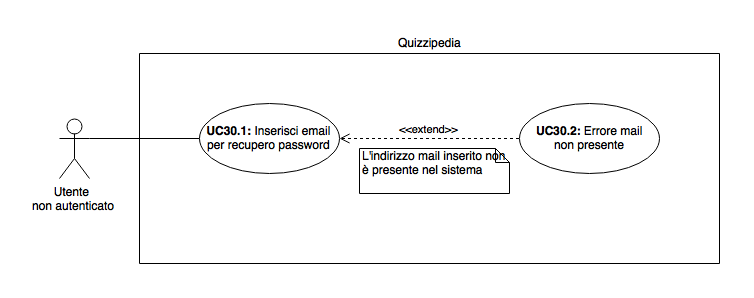
\includegraphics[width=\textwidth]{../img/diagramUC30.png}
	\caption{Caso d'uso UC30: Recupero password}\label{fig:UC30} 
\end{figure}
\begin{itemize}

\item \textbf{Attore}: Utente non autenticato; 
\item \textbf{Precondizione}: L'utente è registrato nel sistema ma non ricorda la password;

\item \textbf{Flusso principale degli eventi}:
\begin{enumerate}
	\item L'utente inserisce l'indirizzo email con il quale si è registrato (\hyperlink{UC30.1}{UC30.1});
	\item L'utente seleziona la funzionalità che spedirà al proprio indirizzo email una nuova password temporanea;
	
\end{enumerate}
\item \textbf{Postcondizione}: L'utente ha recuperato la password.
\end{itemize}
\hypertarget{UC30.1}{}
\subsection{Caso d'uso UC30.1: Inserisci mail per recupero password}

\begin{itemize}

\item \textbf{Attore}: Utente non autenticato; 
\item \textbf{Precondizione}: L'utente è registrato presso il sistema;

\item \textbf{Flusso principale degli eventi}:
\begin{enumerate}
	\item L'utente inserisce correttamente la sua email;
	
\end{enumerate}
\item \textbf{Estensioni}:
\begin{enumerate}
	\item Se l'indirizzo email non è presente nel sistema viene visualizzato un messaggio di errore (\hyperlink{UC30.2}{UC30.2});
	
\end{enumerate}
\item \textbf{Postcondizione}: L'utente ha inserito la mail.
\end{itemize}
\hypertarget{UC30.2}{}
\subsection{Caso d'uso UC30.2: Errore mail non presente}

\begin{itemize}

\item \textbf{Attore}: Utente non autenticato; 
\item \textbf{Precondizione}: L'indirizzo mail inserito non è presente nel sistema;

\item \textbf{Flusso principale degli eventi}:
\begin{enumerate}
	\item Viene visualizzato un messaggio di errore;
	
\end{enumerate}
\item \textbf{Postcondizione}: L'utente non può recuperare la password.
\end{itemize}
\hypertarget{UC31}{}
\subsection{Caso d'uso UC31: Gestione argomenti}
\begin{figure}[H]
	\centering
	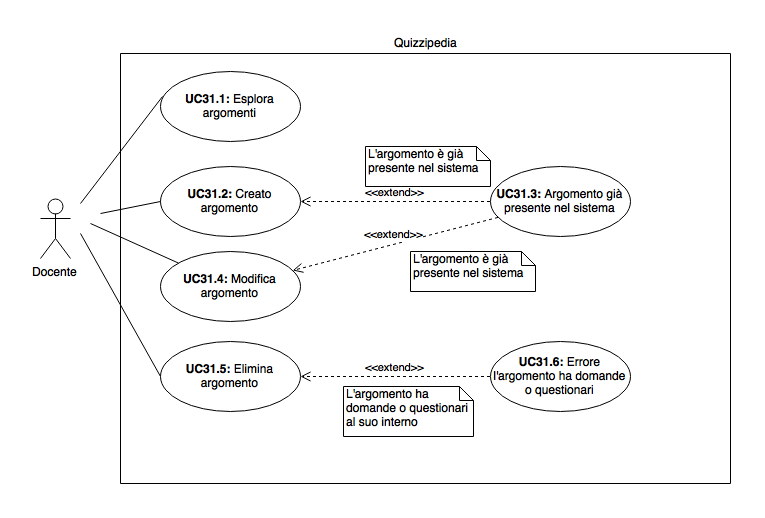
\includegraphics[width=\textwidth]{../img/diagramUC31.png}
	\caption{Caso d'uso UC31: Gestione argomenti}\label{fig:UC31} 
\end{figure}
\begin{itemize}

\item \textbf{Attore}: Docente; 
\item \textbf{Precondizione}: Il docente è autenticato nel sistema;

\item \textbf{Flusso principale degli eventi}:
\begin{enumerate}
	\item Il docente può esplorare gli argomenti (\hyperlink{UC31.1}{UC31.1});
	\item Il docente può creare un argomento (\hyperlink{UC31.2}{UC31.2});
	\item Il docente può modificare un argomento (\hyperlink{UC31.4}{UC31.4});
	\item Il docente può eliminare un argomento (\hyperlink{UC31.5}{UC31.5});
	
\end{enumerate}
\item \textbf{Postcondizione}: Il sistema ha ottenuto le informazioni sulle operazioni che il docente desidera eseguire su un argomento.
\end{itemize}
\hypertarget{UC31.1}{}
\subsection{Caso d'uso UC31.1: Esplora argomenti}

\begin{itemize}

\item \textbf{Attore}: Docente; 
\item \textbf{Precondizione}: Il docente è autenticato nel sistema;

\item \textbf{Flusso principale degli eventi}:
\begin{enumerate}
	\item Il docente visualizza l'albero degli argomenti;
	
\end{enumerate}
\item \textbf{Postcondizione}: Il docente visualizza l'albero degli argomenti.
\end{itemize}
\hypertarget{UC31.2}{}
\subsection{Caso d'uso UC31.2: Crea argomento}

\begin{itemize}

\item \textbf{Attore}: Docente; 
\item \textbf{Precondizione}: Il docente è autenticato nel sistema;

\item \textbf{Flusso principale degli eventi}:
\begin{enumerate}
	\item Il docente inserisce il nome dell'argomento;
	\item Il docente seleziona l'argomento padre (\hyperlink{UC31.1}{UC31.1});
	\item Il docente conferma la creazione dell'argomento;
	
\end{enumerate}
\item \textbf{Estensioni}:
\begin{enumerate}
	\item Se l'argomento già presente nel sistema viene visualizzato un messaggio di errore (\hyperlink{UC31.3}{UC31.3});
	
\end{enumerate}
\item \textbf{Postcondizione}: È inserito un nuovo argomento.
\end{itemize}
\hypertarget{UC31.3}{}
\subsection{Caso d'uso UC31.3: Argomento già presente nel sistema}

\begin{itemize}

\item \textbf{Attore}: Docente; 
\item \textbf{Precondizione}: L'argomento è già presente nel sistema;

\item \textbf{Flusso principale degli eventi}:
\begin{enumerate}
	\item Viene visualizzato un messaggio d'errore;
	
\end{enumerate}
\item \textbf{Postcondizione}: L'argomento non viene inserito nel sistema.
\end{itemize}
\hypertarget{UC31.4}{}
\subsection{Caso d'uso UC31.4: Modifica argomento}

\begin{itemize}

\item \textbf{Attore}: Docente; 
\item \textbf{Precondizione}: Il docente è autenticato nel sistema;

\item \textbf{Flusso principale degli eventi}:
\begin{enumerate}
	\item Il docente seleziona un argomento da modificare (\hyperlink{UC31.1}{UC31.1});
	\item Il docente può modificare il nome dell'argomento;
	\item Il docente può cambiare l'argomento padre (\hyperlink{UC31.1}{UC31.1});
	\item Il docente conferma la modifica dell'argomento;
	
\end{enumerate}
\item \textbf{Estensioni}:
\begin{enumerate}
	\item Se l'argomento già presente nel sistema viene visualizzato un messaggio di errore (\hyperlink{UC31.3}{UC31.3});
	
\end{enumerate}
\item \textbf{Postcondizione}: È stato modificato un argomento.
\end{itemize}
\hypertarget{UC31.5}{}
\subsection{Caso d'uso UC31.5: Elimina argomento}

\begin{itemize}

\item \textbf{Attore}: Docente; 
\item \textbf{Precondizione}: Il docente è autenticato nel sistema;

\item \textbf{Flusso principale degli eventi}:
\begin{enumerate}
	\item Il docente seleziona l'argomento da eliminare (\hyperlink{UC31.1}{UC31.1});
	\item Il docente conferma l'eliminazione;
	
\end{enumerate}
\item \textbf{Estensioni}:
\begin{enumerate}
	\item Se l'argomento ha domande o questionari viene visualizzato un messaggio d'errore (\hyperlink{UC31.6}{UC31.6});
	
\end{enumerate}
\item \textbf{Postcondizione}: È stato eliminato un argomento.
\end{itemize}
\hypertarget{UC31.6}{}
\subsection{Caso d'uso UC31.6: Errore l'argomento ha domande o questionari}

\begin{itemize}

\item \textbf{Attore}: Docente; 
\item \textbf{Precondizione}: L'argomento ha domande o questionari al suo interno;

\item \textbf{Flusso principale degli eventi}:
\begin{enumerate}
	\item Viene visualizzato un messaggio d'errore;
	
\end{enumerate}
\item \textbf{Postcondizione}: L'argomento non viene eliminato.
\end{itemize}
\hypertarget{UC32}{}
\subsection{Caso d'uso UC32: Storico studente}
\begin{figure}[H]
	\centering
	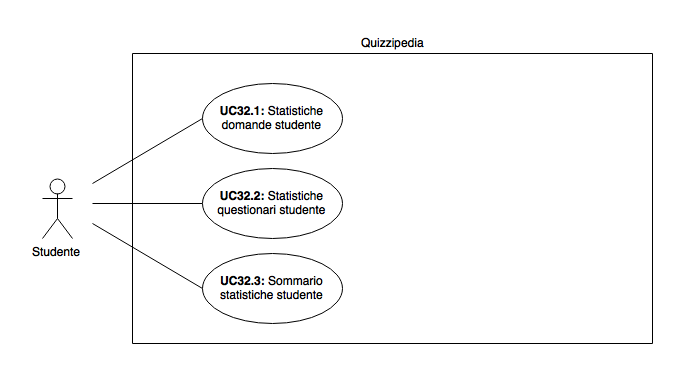
\includegraphics[width=\textwidth]{../img/diagramUC32.png}
	\caption{Caso d'uso UC32: Storico studente}\label{fig:UC32} 
\end{figure}
\begin{itemize}

\item \textbf{Attore}: Studente; 
\item \textbf{Precondizione}: Lo studente è autenticato presso il sistema;

\item \textbf{Flusso principale degli eventi}:
\begin{enumerate}
	\item Lo studente può visualizzare le sue risposte e le statistiche generali relative alle domande eseguite (\hyperlink{UC32.1}{UC32.1});
	\item Lo studente può visualizzare le sue risposte e le statistiche generali relative ai questionari eseguiti (\hyperlink{UC32.2}{UC32.2});
	\item Lo studente può visualizzare un sommario delle proprie statistiche (\hyperlink{UC32.3}{UC32.3});
	
\end{enumerate}
\item \textbf{Postcondizione}: Lo studente ha visualizzato le sue risposte e le statistiche generali relative ai test eseguiti.
\end{itemize}
\hypertarget{UC32.1}{}
\subsection{Caso d'uso UC32.1: Statistiche domande studente}

\begin{itemize}

\item \textbf{Attore}: Studente; 
\item \textbf{Precondizione}: Lo studente è autenticato presso il sistema;

\item \textbf{Flusso principale degli eventi}:
\begin{enumerate}
	\item Lo studente cerca una domanda tra quelle che ha eseguito in passato (\hyperlink{UC11}{UC11});
	\item Lo studente seleziona la domanda per visualizzarne le risposte date e le statistiche generali;
	
\end{enumerate}
\item \textbf{Postcondizione}: Lo studente ha visualizzato i risultati e le statistiche relative alle domande desiderate.
\end{itemize}
\hypertarget{UC32.2}{}
\subsection{Caso d'uso UC32.2: Statistiche questionari studente}

\begin{itemize}

\item \textbf{Attore}: Studente; 
\item \textbf{Precondizione}: Lo studente è autenticato presso il sistema;

\item \textbf{Flusso principale degli eventi}:
\begin{enumerate}
	\item Lo studente cerca un questionario tra quelli che ha eseguito in passato (\hyperlink{UC9}{UC9});
	\item Lo studente seleziona il questionario per visualizzarne le risposte date e le statistiche generali;
	
\end{enumerate}
\item \textbf{Postcondizione}: Lo studente ha visualizzato i risultati e le statistiche relative ai questionari desiderati.
\end{itemize}
\hypertarget{UC32.3}{}
\subsection{Caso d'uso UC32.3: Sommario statistiche studente}

\begin{itemize}

\item \textbf{Attore}: Studente; 
\item \textbf{Precondizione}: Lo studente è autenticato presso il sistema;

\item \textbf{Flusso principale degli eventi}:
\begin{enumerate}
	\item Lo studente visualizza un sommario delle proprie statistiche;
	
\end{enumerate}
\item \textbf{Postcondizione}: Lo studente ha visualizzato i risultati e le statistiche relative alle domande desiderate.
\end{itemize}

\newpage
\section{Requisiti}
\subsection{Struttura di un requisito}
È compito degli \ANpl\ stilare una lista dei requisiti emersi dal capitolato e da eventuali riunioni con il proponente. Questi requisiti dovranno essere classificati per tipo e importanza, utilizzando la seguente struttura:
\begin{center}
	R[importanza][tipo][codice]
\end{center}
\begin{itemize}
	\item \textbf{Importanza} può assumere i seguenti valori:
	\begin{description}
		\item[1:] requisito desiderabile
		\item[2:] requisito opzionale
		\item[3:] requisito obbligatorio
	\end{description}
	\item \textbf{Tipo} può assumere i seguenti valori:
	\begin{description}
		\item[F:] Funzionale, descrive i servizi o le funzioni offerte dal sistema
		\item[Q:] Di Qualità, descrive i requisiti sulla qualità offerte dal sistema
		\item[P:] Prestazionale, descrive i requisiti sulle prestazioni offerte dal sistema
		\item[V:] Vincolo, descrive i vincoli sui servizi offerti dal sistema
	\end{description}
	\item \textbf{Codice} è un numero progressivo univoco per ogni requisito, indipendente da importanza e tipo. Nel caso si abbia un sotto-requisito codice può anche essere espresso in modo gerarchico tramite la notazione:
	\begin{center}
		\textit{CodiceRequistoPadre.CodiceSottorequisito}
	\end{center}
	\item \textbf{Validazione:} verrà inserito un link al metodo deciso per validare il requisito
\end{itemize}
Ogni requisito deve essere correlato da una sintetica ma precisa descrizione. Per ogni requisito bisogna indicarne le fonti, che posso essere il capitolato o uno o più casi d'uso.

\subsection{Tabella dei requisiti}

\begin{longtable}{p{0.04\textwidth} l p{0.15\textwidth} p{6cm} p{0.12\textwidth}}
	\toprule
	\multicolumn{2}{c}{Requisito} & Tipologia & Descrizione & Fonti\tabularnewline
	\midrule
	\midrule
	& \hypertarget{R-3V1}{R-3V1} & Vincolo
	
	Obbligatorio & La parte destinata ai creatori di domande e di questionari dovrà essere fruibile attraverso un PC & Capitolato\tabularnewline
	\midrule
	& \hypertarget{R-3V2}{R-3V2} & Vincolo
	
	Obbligatorio & La parte server deve essere realizzata in Java con server Tomcat o Javascript con server Node.js
	& Capitolato\tabularnewline
	\hline
	& \hypertarget{R-3V3}{R-3V3} & Vincolo
	
	Obbligatorio & La parte client dovrà essere eseguibile in un browser HTML5 & Capitolato\tabularnewline
	\hline
	\begin{tikzpicture}
	\draw [->, thick] (0.2,0.2) -- (0.2,0.1) -- (1,0.1);
	\end{tikzpicture} & \hypertarget{R-3V3.1}{R-3V3.1} & Vincolo
	
	Obbligatorio & L'applicazione funziona correttamente su Chrome versione 47.0.2526 e successive & Capitolato\tabularnewline
	\hline
	\begin{tikzpicture}
	\draw [->, thick] (0.2,0.2) -- (0.2,0.1) -- (1,0.1);
	\end{tikzpicture} & \hypertarget{R-3V3.2}{R-3V3.2} & Vincolo
	
	Obbligatorio & L'applicazione funziona correttamente su Firefox versione 38.5.2esr e successive & Capitolato\tabularnewline
	\hline
	\begin{tikzpicture}
	\draw [->, thick] (0.2,0.2) -- (0.2,0.1) -- (1,0.1);
	\end{tikzpicture} & \hypertarget{R-3V3.3}{R-3V3.3} & Vincolo
	
	Obbligatorio & L'applicazione funziona correttamente su Microsoft Edge versione 25.10586 e successive & Capitolato\tabularnewline
	\hline
	\begin{tikzpicture}
	\draw [->, thick] (0.2,0.2) -- (0.2,0.1) -- (1,0.1);
	\end{tikzpicture} & \hypertarget{R-3V3.4}{R-3V3.4} & Vincolo
	
	Obbligatorio & L'applicazione funziona correttamente su Safari versione 9.0.2 e successive & Capitolato\tabularnewline
	\hline
	& \hypertarget{R-3V4}{R-3V4} & Vincolo
	
	Obbligatorio & L'applicazione deve utilizzare fogli stile CSS per l’ aspetto estetico & Capitolato\tabularnewline
	\hline
	& \hypertarget{R-3V5}{R-3V5} & Vincolo
	
	Obbligatorio & L'applicazione deve utilizzare Javascript per la parte attiva del client & Capitolato\tabularnewline
	\hline
	& \hypertarget{R-3V6}{R-3V6} & Vincolo
	
	Obbligatorio & La parte destinata agli esaminandi dovrà funzionare con qualunque dispositivo: dal Personal Computer, ai Tablet ed agli SmartPhone & Capitolato\tabularnewline
	\hline
	\begin{tikzpicture}
	\draw [->, thick] (0.2,0.2) -- (0.2,0.1) -- (1,0.1);
	\end{tikzpicture} & \hypertarget{R-3V6.1}{R-3V6.1} & Vincolo
	
	Obbligatorio & La parte destinata agli esaminandi dovrà funzionare si smartphone e tablet iOS dalla versione iOS6 & Capitolato\tabularnewline
	\hline
	\begin{tikzpicture}
	\draw [->, thick] (0.2,0.2) -- (0.2,0.1) -- (1,0.1);
	\end{tikzpicture} & \hypertarget{R-3V6.2}{R-3V6.2} & Vincolo
	
	Obbligatorio & La parte destinata agli esaminandi dovrà funzionare su Android dalla versione 4.0 & Capitolato\tabularnewline
	\hline
	& \hypertarget{R-3F7}{R-3F7} & Funzionale
	
	Obbligatorio & Il sistema deve gestire questionari & Capitolato
	
	\hyperlink{UC6}{UC6}\tabularnewline
	\hline
	\begin{tikzpicture}
	\draw [->, thick] (0.2,0.2) -- (0.2,0.1) -- (1,0.1);
	\end{tikzpicture} & \hypertarget{R-3F7.1}{R-3F7.1} & Funzionale
	
	Obbligatorio & L'applicazione deve archiviare quiz in un server, suddivisi per argomento
	& Capitolato\tabularnewline
	\hline
	\begin{tikzpicture}
	\draw [->, thick] (0.2,0.2) -- (0.2,0.1) -- (1,0.1);
	\end{tikzpicture} & \hypertarget{R-3F7.2}{R-3F7.2} & Funzionale
	
	Obbligatorio & L'applicazione deve poter archiviare questionari contenenti domande & Capitolato\tabularnewline
	\hline
	\begin{tikzpicture}
	\draw [->, thick] (0.2,0.2) -- (0.2,0.1) -- (1,0.1);
	\end{tikzpicture} & \hypertarget{R-3F7.3}{R-3F7.3} & Funzionale
	
	Obbligatorio & L'applicazione deve tradurre da QML a HTML le domande archiviate & Capitolato\tabularnewline
	\hline
	\begin{tikzpicture}
	\draw [->, thick] (0.2,0.2) -- (0.2,0.1) -- (1,0.1);
	\end{tikzpicture} & \hypertarget{R-3F7.4}{R-3F7.4} & Funzionale
	
	Obbligatorio & L'applicazione deve proporre questionari preconfezionati & Capitolato\tabularnewline
	\hline
	\begin{tikzpicture}
	\draw [->, thick] (0.2,0.2) -- (0.2,0.1) -- (1,0.1);
	\end{tikzpicture} & \hypertarget{R-3F7.5}{R-3F7.5} & Funzionale
	
	Obbligatorio & L'applicazione deve valutare le risposte fornite dall'utente & Capitolato
	
	\hyperlink{UC32}{UC32}\tabularnewline
	\hline
	\begin{tikzpicture}
	\draw [->, thick] (0.2,0.2) -- (0.2,0.1) -- (1,0.1);
	\end{tikzpicture} & \hypertarget{R-3F7.6}{R-3F7.6} & Funzionale
	
	Obbligatorio & Le domande dovranno essere raccolte attraverso uno specifico linguaggio, che chiameremo Quiz Markup Language (QML), studiato per descrivere quiz
	& Capitolato\tabularnewline
	\hline
	\begin{tikzpicture}
	\draw [->, thick] (0.4,0.2) -- (0.4,0.1) -- (1,0.1);
	\end{tikzpicture} & \hypertarget{R-3F7.6.1}{R-3F7.6.1} & Funzionale
	
	Obbligatorio & Il QML deve gestire risposte vero/falso, risposte a scelta multipla, testi e immagini & Capitolato\tabularnewline
	\hline
	\begin{tikzpicture}
	\draw [->, thick] (0.4,0.2) -- (0.4,0.1) -- (1,0.1);
	\end{tikzpicture} & \hypertarget{R-3F7.6.2}{R-3F7.6.2} & Funzionale
	
	Obbligatorio & Le domande scritte in QML devono essere editabili dall'utente & Proponente\tabularnewline
	\hline
	\begin{tikzpicture}
	\draw [->, thick] (0.4,0.2) -- (0.4,0.1) -- (1,0.1);
	\end{tikzpicture} & \hypertarget{R-2F7.6.3}{R-2F7.6.3} & Funzionale
	
	Opzionale & Le domande possono essere inserite e editabili attraverso interfaccia grafica & Proponente\tabularnewline
	\hline
	\begin{tikzpicture}
	\draw [->, thick] (0.2,0.2) -- (0.2,0.1) -- (1,0.1);
	\end{tikzpicture} & \hypertarget{R-3F7.7}{R-3F7.7} & Funzionale
	
	Obbligatorio & Il sistema deve gestire sia questionari pubblici che privati & Proponente\tabularnewline
	\hline
	\begin{tikzpicture}
	\draw [->, thick] (0.2,0.2) -- (0.2,0.1) -- (1,0.1);
	\end{tikzpicture} & \hypertarget{R-3F7.8}{R-3F7.8} & Funzionale
	
	Obbligatorio & I docenti costruiranno questionari scegliendo tra le domande archiviate nel server & Capitolato
	
	\hyperlink{UC6.1}{UC6.1}
	
	\hyperlink{UC6}{UC6}\tabularnewline
	\hline
	\begin{tikzpicture}
	\draw [->, thick] (0.4,0.2) -- (0.4,0.1) -- (1,0.1);
	\end{tikzpicture} & \hypertarget{R-3F7.8.1}{R-3F7.8.1} & Funzionale
	
	Obbligatorio & Il sistema deve segnalare un errore nel caso un questionario creato non contenga domande & \hyperlink{UC6.1}{UC6.1}
	
	\hyperlink{UC6.7}{UC6.7}
	
	\hyperlink{UC6}{UC6}\tabularnewline
	\hline
	\begin{tikzpicture}
	\draw [->, thick] (0.2,0.2) -- (0.2,0.1) -- (1,0.1);
	\end{tikzpicture} & \hypertarget{R-2F7.9}{R-2F7.9} & Funzionale
	
	Opzionale & il sistema deve offrire la possibilità di creare dinamicamente i questionari & Capitolato\tabularnewline
	\hline
	\begin{tikzpicture}
	\draw [->, thick] (0.2,0.2) -- (0.2,0.1) -- (1,0.1);
	\end{tikzpicture} & \hypertarget{R-2F7.10}{R-2F7.10} & Funzionale
	
	Opzionale & Il l'applicazione deve essere predisposta ad un sistema di feedback per le domande & Capitolato\tabularnewline
	\hline
	\begin{tikzpicture}
	\draw [->, thick] (0.2,0.2) -- (0.2,0.1) -- (1,0.1);
	\end{tikzpicture} & \hypertarget{R-3F7.11}{R-3F7.11} & Funzionale
	
	Obbligatorio & Il sistema deve permettere la raccolta dei dati relativi a questionari svolti & Capitolato\tabularnewline
	\hline
	\begin{tikzpicture}
	\draw [->, thick] (0.4,0.2) -- (0.4,0.1) -- (1,0.1);
	\end{tikzpicture} & \hypertarget{R-3F7.11.1}{R-3F7.11.1} & Funzionale
	
	Obbligatorio & Il sistema deve permettere la rivisitazione del test svolto e dei risultati ottenuti & Capitolato
	
	\hyperlink{UC32}{UC32}\tabularnewline
	\hline
	\begin{tikzpicture}
	\draw [->, thick] (0.4,0.2) -- (0.4,0.1) -- (1,0.1);
	\end{tikzpicture} & \hypertarget{R-3F7.11.2}{R-3F7.11.2} & Funzionale
	
	Obbligatorio & Il sistema deve offrire la possibilità di analizzare i dati raccolti dai test effettuati & Capitolato\tabularnewline
	\hline
	\begin{tikzpicture}
	\draw [->, thick] (0.4,0.2) -- (0.4,0.1) -- (1,0.1);
	\end{tikzpicture} & \hypertarget{R-2F7.11.3}{R-2F7.11.3} & Funzionale
	
	Opzionale & Il sistema deve offrire la possibilità di visualizzazione sotto forma di grafico delle statistiche i dati raccolti & Capitolato\tabularnewline
	\hline
	\begin{tikzpicture}
	\draw [->, thick] (0.2,0.2) -- (0.2,0.1) -- (1,0.1);
	\end{tikzpicture} & \hypertarget{R-3F7.12}{R-3F7.12} & Funzionale
	
	Obbligatorio & Il sistema deve prevedere la gestione di domande & \hyperlink{UC6.4}{UC6.4}
	
	\hyperlink{UC6.5}{UC6.5}
	
	\hyperlink{UC6}{UC6}
	
	\hyperlink{UC7}{UC7}\tabularnewline
	\hline
	\begin{tikzpicture}
	\draw [->, thick] (0.4,0.2) -- (0.4,0.1) -- (1,0.1);
	\end{tikzpicture} & \hypertarget{R-3F7.12.1}{R-3F7.12.1} & Funzionale
	
	Obbligatorio & Il sistema deve consentire ad un docente di inserire una nuova domanda & \hyperlink{UC7.1}{UC7.1}
	
	\hyperlink{UC7}{UC7}\tabularnewline
	\hline
	\begin{tikzpicture}
	\draw [->, thick] (0.6,0.2) -- (0.6,0.1) -- (1,0.1);
	\end{tikzpicture} & \hypertarget{R-3F7.12.1.1}{R-3F7.12.1.1} & Funzionale
	
	Obbligatorio & Un docente deve poter selezionare gli argomenti di una domanda & \hyperlink{UC7.1}{UC7.1}
	
	\hyperlink{UC7.4}{UC7.4}
	
	\hyperlink{UC7}{UC7}\tabularnewline
	\hline
	\begin{tikzpicture}
	\draw [->, thick] (0.8,0.2) -- (0.8,0.1) -- (1,0.1);
	\end{tikzpicture} & \hypertarget{R-3F7.12.1.1.1}{R-3F7.12.1.1.1} & Funzionale
	
	Obbligatorio & Il sistema deve segnalare un errore nel caso non venga selezionato alcun argomento per una nuova domanda & \hyperlink{UC6.4}{UC6.4}
	
	\hyperlink{UC7.4}{UC7.4}
	
	\hyperlink{UC7.7}{UC7.7}
	
	\hyperlink{UC7}{UC7}\tabularnewline
	\hline
	\begin{tikzpicture}
	\draw [->, thick] (0.6,0.2) -- (0.6,0.1) -- (1,0.1);
	\end{tikzpicture} & \hypertarget{R-3F7.12.1.2}{R-3F7.12.1.2} & Funzionale
	
	Obbligatorio & Un docente deve comporre la domanda da inserire in QML & \hyperlink{UC6.4}{UC6.4}
	
	\hyperlink{UC7.5}{UC7.5}
	
	\hyperlink{UC7}{UC7}\tabularnewline
	\hline
	\begin{tikzpicture}
	\draw [->, thick] (0.8,0.2) -- (0.8,0.1) -- (1,0.1);
	\end{tikzpicture} & \hypertarget{R-3F7.12.1.2.1}{R-3F7.12.1.2.1} & Funzionale
	
	Obbligatorio & Il sistema deve segnalare un errore nel caso di inserimento QML non valido & \hyperlink{UC6.4}{UC6.4}
	
	\hyperlink{UC7.5}{UC7.5}
	
	\hyperlink{UC7.6}{UC7.6}
	
	\hyperlink{UC7}{UC7}\tabularnewline
	\hline
	\begin{tikzpicture}
	\draw [->, thick] (0.4,0.2) -- (0.4,0.1) -- (1,0.1);
	\end{tikzpicture} & \hypertarget{R-3F7.12.2}{R-3F7.12.2} & Funzionale
	
	Obbligatorio & Il sistema deve consentire ad un docente di modificare una domanda & \hyperlink{UC7.2}{UC7.2}
	
	\hyperlink{UC7}{UC7}\tabularnewline
	\hline
	\begin{tikzpicture}
	\draw [->, thick] (0.4,0.2) -- (0.4,0.1) -- (1,0.1);
	\end{tikzpicture} & \hypertarget{R-3F7.12.3}{R-3F7.12.3} & Funzionale
	
	Obbligatorio & Il sistema deve consentire ad un docente di eliminare una domanda presente nel sistema & \hyperlink{UC7.3}{UC7.3}
	
	\hyperlink{UC7}{UC7}\tabularnewline
	\hline
	\begin{tikzpicture}
	\draw [->, thick] (0.2,0.2) -- (0.2,0.1) -- (1,0.1);
	\end{tikzpicture} & \hypertarget{R-3F7.13}{R-3F7.13} & Funzionale
	
	Obbligatorio & il sistema deve dare la possibilità al docente di modificare il proprio questionario & \hyperlink{UC6.2}{UC6.2}
	
	\hyperlink{UC6}{UC6}\tabularnewline
	\hline
	\begin{tikzpicture}
	\draw [->, thick] (0.4,0.2) -- (0.4,0.1) -- (1,0.1);
	\end{tikzpicture} & \hypertarget{R-3F7.13.1}{R-3F7.13.1} & Funzionale
	
	Obbligatorio & Il sistema deve dare la possibilità di ricercare un questionario & \hyperlink{UC9}{UC9}\tabularnewline
	\hline
	\begin{tikzpicture}
	\draw [->, thick] (0.4,0.2) -- (0.4,0.1) -- (1,0.1);
	\end{tikzpicture} & \hypertarget{R-3F7.13.2}{R-3F7.13.2} & Funzionale
	
	Obbligatorio & Il sistema deve dare la possibile al docente di aggiungere al questionario già fatto una domanda. & \hyperlink{UC6.4}{UC6.4}
	
	\hyperlink{UC6}{UC6}\tabularnewline
	\hline
	\begin{tikzpicture}
	\draw [->, thick] (0.4,0.2) -- (0.4,0.1) -- (1,0.1);
	\end{tikzpicture} & \hypertarget{R-3F7.13.3}{R-3F7.13.3} & Funzionale
	
	Obbligatorio & Il sistema deve dare la possibilità al docente di togliere domande precedentemente aggiunte al questionario & \hyperlink{UC6.5}{UC6.5}
	
	\hyperlink{UC6}{UC6}\tabularnewline
	\hline
	\begin{tikzpicture}
	\draw [->, thick] (0.4,0.2) -- (0.4,0.1) -- (1,0.1);
	\end{tikzpicture} & \hypertarget{R-3F7.13.4}{R-3F7.13.4} & Funzionale
	
	Obbligatorio & Il sistema deve consentire ad un docente di modificare gli argomenti di un proprio questionario & \hyperlink{UC6.2}{UC6.2}
	
	\hyperlink{UC6.6}{UC6.6}
	
	\hyperlink{UC6}{UC6}\tabularnewline
	\hline
	\begin{tikzpicture}
	\draw [->, thick] (0.2,0.2) -- (0.2,0.1) -- (1,0.1);
	\end{tikzpicture} & \hypertarget{R-3F7.14}{R-3F7.14} & Funzionale
	
	Obbligatorio & Il sistema deve dare la possibilità al docente di eliminare il proprio questionario & \hyperlink{UC6.3}{UC6.3}
	
	\hyperlink{UC6}{UC6}\tabularnewline
	\hline
	& \hypertarget{R-3F8}{R-3F8} & Funzionale
	
	Obbligatorio & Il sistema deve permettere l’autenticazione
	di un utente & \hyperlink{UC2}{UC2}\tabularnewline
	\hline
	\begin{tikzpicture}
	\draw [->, thick] (0.2,0.2) -- (0.2,0.1) -- (1,0.1);
	\end{tikzpicture} & \hypertarget{R-3F8.1}{R-3F8.1} & Funzionale
	
	Obbligatorio & L’autenticazione richiede l’inserimento dell’e-mail e della password & \hyperlink{UC2.1}{UC2.1}
	
	\hyperlink{UC2.2}{UC2.2}
	
	\hyperlink{UC2}{UC2}\tabularnewline
	\hline
	\begin{tikzpicture}
	\draw [->, thick] (0.2,0.2) -- (0.2,0.1) -- (1,0.1);
	\end{tikzpicture} & \hypertarget{R-3F8.2}{R-3F8.2} & Funzionale
	
	Obbligatorio & Il sistema deve permettere la visualizzazione di un messaggio di errore in caso di email o password non valida & \hyperlink{UC2.3}{UC2.3}
	
	\hyperlink{UC2.4}{UC2.4}
	
	\hyperlink{UC2}{UC2}\tabularnewline
	\hline
	& \hypertarget{R-3F9}{R-3F9} & Funzionale
	
	Obbligatorio & Il candidato attraverso una specifica interfaccia potrà rispondere alle domande & Capitolato\tabularnewline
	\hline
	& \hypertarget{R-3F10}{R-3F10} & Funzionale
	
	Obbligatorio & Il sistema deve avere almeno 3 tipi di utenti: amministratore, docente e studente & Capitolato\tabularnewline
	\hline
	& \hypertarget{R-3F11}{R-3F11} & Funzionale
	
	Obbligatorio & Il sistema deve gestire la registrazione di un utente & \hyperlink{UC1}{UC1}\tabularnewline
	\hline
	\begin{tikzpicture}
	\draw [->, thick] (0.2,0.2) -- (0.2,0.1) -- (1,0.1);
	\end{tikzpicture} & \hypertarget{R-3F11.1}{R-3F11.1} & Funzionale
	
	Obbligatorio & Il sistema deve contenere già un account proprietario & Interno\tabularnewline
	\hline
	\begin{tikzpicture}
	\draw [->, thick] (0.2,0.2) -- (0.2,0.1) -- (1,0.1);
	\end{tikzpicture} & \hypertarget{R-3F11.2}{R-3F11.2} & Funzionale
	
	Obbligatorio & Il sistema deve permettere la registrazione
	di uno studente & \hyperlink{UC1}{UC1}\tabularnewline
	\hline
	\begin{tikzpicture}
	\draw [->, thick] (0.4,0.2) -- (0.4,0.1) -- (1,0.1);
	\end{tikzpicture} & \hypertarget{R-3F11.2.1}{R-3F11.2.1} & Funzionale
	
	Obbligatorio & La registrazione di uno studente richiede l’inserimento
	della mail, password, nome e cognome & \hyperlink{UC1.1}{UC1.1}
	
	\hyperlink{UC1.2}{UC1.2}
	
	\hyperlink{UC1.6.1}{UC1.6.1}
	
	\hyperlink{UC1.6.2}{UC1.6.2}
	
	\hyperlink{UC1}{UC1}\tabularnewline
	\hline
	\begin{tikzpicture}
	\draw [->, thick] (0.6,0.2) -- (0.6,0.1) -- (1,0.1);
	\end{tikzpicture} & \hypertarget{R-3F11.2.1.1}{R-3F11.2.1.1} & Funzionale
	
	Obbligatorio & Il sistema deve segnalare un errore nel caso non vengano inseriti tutti i campi necessari per la registrazione & \hyperlink{UC1.6}{UC1.6}
	
	\hyperlink{UC1}{UC1}\tabularnewline
	\hline
	\begin{tikzpicture}
	\draw [->, thick] (0.6,0.2) -- (0.6,0.1) -- (1,0.1);
	\end{tikzpicture} & \hypertarget{R-3F11.2.1.2}{R-3F11.2.1.2} & Funzionale
	
	Obbligatorio & La registrazione di uno studente deve richiedere l'inserimento delle informazioni personali & \hyperlink{UC1.6}{UC1.6}
	
	\hyperlink{UC1}{UC1}\tabularnewline
	\hline
	\begin{tikzpicture}
	\draw [->, thick] (0.8,0.2) -- (0.8,0.1) -- (1,0.1);
	\end{tikzpicture} & \hypertarget{R-3F11.2.1.2.1}{R-3F11.2.1.2.1} & Funzionale
	
	Obbligatorio & Il sistema deve segnalare un errore se non sono state inserite tutte le informazioni personali richieste & \hyperlink{UC1.6}{UC1.6}
	
	\hyperlink{UC1.7}{UC1.7}
	
	\hyperlink{UC1}{UC1}\tabularnewline
	\hline
	\begin{tikzpicture}
	\draw [->, thick] (0.6,0.2) -- (0.6,0.1) -- (1,0.1);
	\end{tikzpicture} & \hypertarget{R-3F11.2.1.3}{R-3F11.2.1.3} & Funzionale
	
	Obbligatorio & Il sistema deve richiedere di ripetere l'inserimento della password durante la registrazione di uno studente & \hyperlink{UC1.8}{UC1.8}
	
	\hyperlink{UC1}{UC1}\tabularnewline
	\hline
	\begin{tikzpicture}
	\draw [->, thick] (0.4,0.2) -- (0.4,0.1) -- (1,0.1);
	\end{tikzpicture} & \hypertarget{R-3F11.2.2}{R-3F11.2.2} & Funzionale
	
	Obbligatorio & Il sistema deve permettere la visualizzazione di un messaggio di errore se la mail dello studente è già presente nel sistema & \hyperlink{UC1.5}{UC1.5}
	
	\hyperlink{UC1}{UC1}\tabularnewline
	\hline
	\begin{tikzpicture}
	\draw [->, thick] (0.4,0.2) -- (0.4,0.1) -- (1,0.1);
	\end{tikzpicture} & \hypertarget{R-3F11.2.3}{R-3F11.2.3} & Funzionale
	
	Obbligatorio & Il sistema deve permettere la visualizzazione di un messaggio di errore se la password dello studente è troppo corta & \hyperlink{UC1.3}{UC1.3}
	
	\hyperlink{UC1}{UC1}\tabularnewline
	\hline
	\begin{tikzpicture}
	\draw [->, thick] (0.4,0.2) -- (0.4,0.1) -- (1,0.1);
	\end{tikzpicture} & \hypertarget{R-3F11.2.4}{R-3F11.2.4} & Funzionale
	
	Obbligatorio & Il sistema deve segnalare un errore se non viene inserito un indirizzo email valido & \hyperlink{UC1.1}{UC1.1}
	
	\hyperlink{UC1.4}{UC1.4}
	
	\hyperlink{UC1}{UC1}\tabularnewline
	\hline
	\begin{tikzpicture}
	\draw [->, thick] (0.4,0.2) -- (0.4,0.1) -- (1,0.1);
	\end{tikzpicture} & \hypertarget{R-3F11.2.5}{R-3F11.2.5} & Funzionale
	
	Obbligatorio & Il sistema deve segnalare un errore se il secondo inserimento password non coincide con il primo & \hyperlink{UC1.8}{UC1.8}
	
	\hyperlink{UC1.9}{UC1.9}
	
	\hyperlink{UC1}{UC1}\tabularnewline
	\hline
	\begin{tikzpicture}
	\draw [->, thick] (0.2,0.2) -- (0.2,0.1) -- (1,0.1);
	\end{tikzpicture} & \hypertarget{R-3F11.3}{R-3F11.3} & Funzionale
	
	Obbligatorio & L'amministratore deve poter inviare un invito di registrazione ad un docente di cui conosce l'indirizzo email & \hyperlink{UC3.1}{UC3.1}
	
	\hyperlink{UC3}{UC3}\tabularnewline
	\hline
	\begin{tikzpicture}
	\draw [->, thick] (0.2,0.2) -- (0.2,0.1) -- (1,0.1);
	\end{tikzpicture} & \hypertarget{R-3F11.4}{R-3F11.4} & Funzionale
	
	Obbligatorio & Il sistema deve poter registrate un docente che ha ricevuto un invito di registrazione & \hyperlink{UC1}{UC1}\tabularnewline
	\hline
	\begin{tikzpicture}
	\draw [->, thick] (0.4,0.2) -- (0.4,0.1) -- (1,0.1);
	\end{tikzpicture} & \hypertarget{R-3F11.4.1}{R-3F11.4.1} & Funzionale
	
	Obbligatorio & La registrazione di un docente richiede l’inserimento della mail, password, nome e cognome & \hyperlink{UC1.1}{UC1.1}
	
	\hyperlink{UC1.2}{UC1.2}
	
	\hyperlink{UC1.6.1}{UC1.6.1}
	
	\hyperlink{UC1.6.2}{UC1.6.2}
	
	\hyperlink{UC1}{UC1}\tabularnewline
	\hline
	\begin{tikzpicture}
	\draw [->, thick] (0.4,0.2) -- (0.4,0.1) -- (1,0.1);
	\end{tikzpicture} & \hypertarget{R-3F11.4.2}{R-3F11.4.2} & Funzionale
	
	Obbligatorio & Il sistema deve permettere la visualizzazione di un messaggio di errore se la mail del docente è già presente nel sistema & \hyperlink{UC1.5}{UC1.5}
	
	\hyperlink{UC1}{UC1}\tabularnewline
	\hline
	\begin{tikzpicture}
	\draw [->, thick] (0.4,0.2) -- (0.4,0.1) -- (1,0.1);
	\end{tikzpicture} & \hypertarget{R-3F11.4.3}{R-3F11.4.3} & Funzionale
	
	Obbligatorio & Il sistema deve permettere la visualizzazione di un messaggio di errore se la password del docente è troppo corta & \hyperlink{UC1.3}{UC1.3}
	
	\hyperlink{UC1}{UC1}\tabularnewline
	\hline
	\begin{tikzpicture}
	\draw [->, thick] (0.2,0.2) -- (0.2,0.1) -- (1,0.1);
	\end{tikzpicture} & \hypertarget{R-3F11.5}{R-3F11.5} & Funzionale
	
	Obbligatorio & Il sistema deve permettere la creazione di un nuovo amministratore da parte del proprietario & \hyperlink{UC25.1}{UC25.1}
	
	\hyperlink{UC25}{UC25}\tabularnewline
	\hline
	& \hypertarget{R-3V12}{R-3V12} & Vincolo
	
	Obbligatorio & Il database server side deve essere SQL (PostgreSQL) oppure noSQL (MongoDB) & Capitolato\tabularnewline
	\hline
	& \hypertarget{R-3F13}{R-3F13} & Funzionale
	
	Obbligatorio & Il sistema deve gestire le azioni di amministratore & \hyperlink{UC3}{UC3}\tabularnewline
	\hline
	\begin{tikzpicture}
	\draw [->, thick] (0.2,0.2) -- (0.2,0.1) -- (1,0.1);
	\end{tikzpicture} & \hypertarget{R-3F13.1}{R-3F13.1} & Funzionale
	
	Obbligatorio & Il sistema deve dare la possibilità ad un amministratore di invitare un docente alla registrazione nel sistema & \hyperlink{UC3.1}{UC3.1}
	
	\hyperlink{UC3}{UC3}\tabularnewline
	\hline
	\begin{tikzpicture}
	\draw [->, thick] (0.2,0.2) -- (0.2,0.1) -- (1,0.1);
	\end{tikzpicture} & \hypertarget{R-3F13.2}{R-3F13.2} & Funzionale
	
	Obbligatorio & Il sistema deve dare la possibilità ad un amministratore la possibilità di rimuovere un docente dal sistema & \hyperlink{UC3.2}{UC3.2}
	
	\hyperlink{UC3}{UC3}\tabularnewline
	\hline
	\begin{tikzpicture}
	\draw [->, thick] (0.2,0.2) -- (0.2,0.1) -- (1,0.1);
	\end{tikzpicture} & \hypertarget{R-3F13.3}{R-3F13.3} & Funzionale
	
	Obbligatorio & Il sistema deve dare la possibilità ad un amministratore di rimuovere uno studente dal sistema  & \hyperlink{UC3.3}{UC3.3}
	
	\hyperlink{UC3}{UC3}\tabularnewline
	\hline
	\begin{tikzpicture}
	\draw [->, thick] (0.2,0.2) -- (0.2,0.1) -- (1,0.1);
	\end{tikzpicture} & \hypertarget{R-3F13.4}{R-3F13.4} & Funzionale
	
	Obbligatorio & Il sistema deve segnalare un errore nel caso un amministratore tenti di inviare un invito ad un indirizzo email già presente nel sistema & \hyperlink{UC3.1}{UC3.1}
	
	\hyperlink{UC3.4}{UC3.4}
	
	\hyperlink{UC3}{UC3}\tabularnewline
	\hline
	& \hypertarget{R-2F14}{R-2F14} & Funzionale
	
	Opzionale & Il sistema deve prevedere la gestione di classi da parte di un docente & \hyperlink{UC5}{UC5}\tabularnewline
	\hline
	\begin{tikzpicture}
	\draw [->, thick] (0.2,0.2) -- (0.2,0.1) -- (1,0.1);
	\end{tikzpicture} & \hypertarget{R-2F14.1}{R-2F14.1} & Funzionale
	
	Opzionale & Un docente deve avere la possibilità di creare una nuova classe & \hyperlink{UC5.1}{UC5.1}
	
	\hyperlink{UC5}{UC5}\tabularnewline
	\hline
	\begin{tikzpicture}
	\draw [->, thick] (0.4,0.2) -- (0.4,0.1) -- (1,0.1);
	\end{tikzpicture} & \hypertarget{R-3F14.1.1}{R-3F14.1.1} & Funzionale
	
	Obbligatorio & Un docente deve poter specificare il nome della nuova classe & \hyperlink{UC5.1}{UC5.1}
	
	\hyperlink{UC5.4}{UC5.4}
	
	\hyperlink{UC5}{UC5}\tabularnewline
	\hline
	\begin{tikzpicture}
	\draw [->, thick] (0.6,0.2) -- (0.6,0.1) -- (1,0.1);
	\end{tikzpicture} & \hypertarget{R-3F14.1.1.1}{R-3F14.1.1.1} & Funzionale
	
	Obbligatorio & Nel caso il nome della classe sia già presente il sistema deve segnalare un errore & \hyperlink{UC5.1}{UC5.1}
	
	\hyperlink{UC5.4}{UC5.4}
	
	\hyperlink{UC5.5}{UC5.5}
	
	\hyperlink{UC5}{UC5}\tabularnewline
	\hline
	\begin{tikzpicture}
	\draw [->, thick] (0.4,0.2) -- (0.4,0.1) -- (1,0.1);
	\end{tikzpicture} & \hypertarget{R-3F14.1.2}{R-3F14.1.2} & Funzionale
	
	Obbligatorio & Un docente deve poter specificare gli argomenti di una nuova classe & \hyperlink{UC5.1}{UC5.1}
	
	\hyperlink{UC5.6}{UC5.6}
	
	\hyperlink{UC5}{UC5}\tabularnewline
	\hline
	\begin{tikzpicture}
	\draw [->, thick] (0.4,0.2) -- (0.4,0.1) -- (1,0.1);
	\end{tikzpicture} & \hypertarget{R-3F14.1.3}{R-3F14.1.3} & Funzionale
	
	Obbligatorio & Un docente deve poter specificare la password relativa ad una nuova classe & \hyperlink{UC5.1}{UC5.1}
	
	\hyperlink{UC5.7}{UC5.7}
	
	\hyperlink{UC5}{UC5}\tabularnewline
	\hline
	\begin{tikzpicture}
	\draw [->, thick] (0.2,0.2) -- (0.2,0.1) -- (1,0.1);
	\end{tikzpicture} & \hypertarget{R-2F14.2}{R-2F14.2} & Funzionale
	
	Opzionale & Un docente deve avere la possibilità di eliminare una classe esistente & \hyperlink{UC5.3}{UC5.3}
	
	\hyperlink{UC5}{UC5}\tabularnewline
	\hline
	\begin{tikzpicture}
	\draw [->, thick] (0.2,0.2) -- (0.2,0.1) -- (1,0.1);
	\end{tikzpicture} & \hypertarget{R-2F14.3}{R-2F14.3} & Funzionale
	
	Opzionale & Un docente deve poter modificare una classe & \hyperlink{UC5.2}{UC5.2}
	
	\hyperlink{UC5}{UC5}\tabularnewline
	\hline
	\begin{tikzpicture}
	\draw [->, thick] (0.4,0.2) -- (0.4,0.1) -- (1,0.1);
	\end{tikzpicture} & \hypertarget{R-3F14.3.1}{R-3F14.3.1} & Funzionale
	
	Obbligatorio & Un docente deve poter modificare il nome di una propria classe esistente & \hyperlink{UC5.2}{UC5.2}
	
	\hyperlink{UC5.4}{UC5.4}
	
	\hyperlink{UC5}{UC5}\tabularnewline
	\hline
	\begin{tikzpicture}
	\draw [->, thick] (0.4,0.2) -- (0.4,0.1) -- (1,0.1);
	\end{tikzpicture} & \hypertarget{R-3F14.3.2}{R-3F14.3.2} & Funzionale
	
	Obbligatorio & Un docente deve poter modificare gli argomenti di una sua classe esistente & \hyperlink{UC5.2}{UC5.2}
	
	\hyperlink{UC5.6}{UC5.6}
	
	\hyperlink{UC5}{UC5}\tabularnewline
	\hline
	\begin{tikzpicture}
	\draw [->, thick] (0.4,0.2) -- (0.4,0.1) -- (1,0.1);
	\end{tikzpicture} & \hypertarget{R-3F14.3.3}{R-3F14.3.3} & Funzionale
	
	Obbligatorio & Un docente deve poter modificare la password di una delle proprie classi & \hyperlink{UC5.2}{UC5.2}
	
	\hyperlink{UC5.7}{UC5.7}
	
	\hyperlink{UC5}{UC5}\tabularnewline
	\hline
	& \hypertarget{R-3F15}{R-3F15} & Funzionale
	
	Obbligatorio & Il sistema deve consentire ad un utente di gestire i propri dati memorizzati nel sistema & \hyperlink{UC10}{UC10}\tabularnewline
	\hline
	\begin{tikzpicture}
	\draw [->, thick] (0.2,0.2) -- (0.2,0.1) -- (1,0.1);
	\end{tikzpicture} & \hypertarget{R-3F15.1}{R-3F15.1} & Funzionale
	
	Obbligatorio & Il sistema deve consentire ad un utente di modificare la propria mail & \hyperlink{UC10.3}{UC10.3}
	
	\hyperlink{UC10}{UC10}\tabularnewline
	\hline
	\begin{tikzpicture}
	\draw [->, thick] (0.4,0.2) -- (0.4,0.1) -- (1,0.1);
	\end{tikzpicture} & \hypertarget{R-3F15.1.1}{R-3F15.1.1} & Funzionale
	
	Obbligatorio & Il sistema deve gestire eventuali errori di inserimento mail  & \hyperlink{UC10.3}{UC10.3}
	
	\hyperlink{UC10.4}{UC10.4}
	
	\hyperlink{UC10}{UC10}\tabularnewline
	\hline
	\begin{tikzpicture}
	\draw [->, thick] (0.4,0.2) -- (0.4,0.1) -- (1,0.1);
	\end{tikzpicture} & \hypertarget{R-3F15.1.2}{R-3F15.1.2} & Funzionale
	
	Obbligatorio & Il sistema deve segnalare un errore in caso di inserimento di email già presente nel sistema & \hyperlink{UC10.3}{UC10.3}
	
	\hyperlink{UC10.5}{UC10.5}
	
	\hyperlink{UC10}{UC10}\tabularnewline
	\hline
	\begin{tikzpicture}
	\draw [->, thick] (0.2,0.2) -- (0.2,0.1) -- (1,0.1);
	\end{tikzpicture} & \hypertarget{R-3F15.2}{R-3F15.2} & Funzionale
	
	Obbligatorio & Il sistema deve consentire ad un utente di modificare la propria password di accesso al sistema & \hyperlink{UC10.2}{UC10.2}
	
	\hyperlink{UC10}{UC10}\tabularnewline
	\hline
	\begin{tikzpicture}
	\draw [->, thick] (0.4,0.2) -- (0.4,0.1) -- (1,0.1);
	\end{tikzpicture} & \hypertarget{R-3F15.2.1}{R-3F15.2.1} & Funzionale
	
	Obbligatorio & Il sistema deve richiedere l'inserimento della vecchia password all'utente per consentire la modifica della password & \hyperlink{UC10.2.1}{UC10.2.1}
	
	\hyperlink{UC10.2.4}{UC10.2.4}
	
	\hyperlink{UC10}{UC10}\tabularnewline
	\hline
	\begin{tikzpicture}
	\draw [->, thick] (0.6,0.2) -- (0.6,0.1) -- (1,0.1);
	\end{tikzpicture} & \hypertarget{R-3F15.2.1.1}{R-3F15.2.1.1} & Funzionale
	
	Obbligatorio & Il sistema deve segnalare l'inserimento di una password scorretta & \hyperlink{UC10.2.4}{UC10.2.4}
	
	\hyperlink{UC10.2}{UC10.2}
	
	\hyperlink{UC10}{UC10}\tabularnewline
	\hline
	\begin{tikzpicture}
	\draw [->, thick] (0.4,0.2) -- (0.4,0.1) -- (1,0.1);
	\end{tikzpicture} & \hypertarget{R-3F15.2.2}{R-3F15.2.2} & Funzionale
	
	Obbligatorio & Il sistema deve richiedere di inserire la nuova password due volte & \hyperlink{UC10.2.3}{UC10.2.3}
	
	\hyperlink{UC10.2}{UC10.2}
	
	\hyperlink{UC10}{UC10}\tabularnewline
	\hline
	\begin{tikzpicture}
	\draw [->, thick] (0.6,0.2) -- (0.6,0.1) -- (1,0.1);
	\end{tikzpicture} & \hypertarget{R-3F15.2.2.1}{R-3F15.2.2.1} & Funzionale
	
	Obbligatorio & Il sistema deve verificare che la nuova password sia di almeno sei caratteri e segnalarlo in caso contrario & \hyperlink{UC10.2.3}{UC10.2.3}
	
	\hyperlink{UC10.2.5}{UC10.2.5}
	
	\hyperlink{UC10.2}{UC10.2}
	
	\hyperlink{UC10}{UC10}\tabularnewline
	\hline
	\begin{tikzpicture}
	\draw [->, thick] (0.6,0.2) -- (0.6,0.1) -- (1,0.1);
	\end{tikzpicture} & \hypertarget{R-3F15.2.2.2}{R-3F15.2.2.2} & Funzionale
	
	Obbligatorio & Il sistema deve controllare che i due campi per l'inserimento della nuova password coincidano e segnalarlo in caso contrario. & \hyperlink{UC10.2.2}{UC10.2.2}
	
	\hyperlink{UC10.2.6}{UC10.2.6}
	
	\hyperlink{UC10.2}{UC10.2}
	
	\hyperlink{UC10}{UC10}\tabularnewline
	\hline
	\begin{tikzpicture}
	\draw [->, thick] (0.2,0.2) -- (0.2,0.1) -- (1,0.1);
	\end{tikzpicture} & \hypertarget{R-3F15.3}{R-3F15.3} & Funzionale
	
	Obbligatorio & Il sistema deve consentire all'utente di modificare i propri dati personali & \hyperlink{UC10.1}{UC10.1}
	
	\hyperlink{UC10}{UC10}\tabularnewline
	\hline
	\begin{tikzpicture}
	\draw [->, thick] (0.4,0.2) -- (0.4,0.1) -- (1,0.1);
	\end{tikzpicture} & \hypertarget{R-3F15.3.1}{R-3F15.3.1} & Funzionale
	
	Obbligatorio & Il sistema deve consentire all'utente la modifica del proprio nome  & \hyperlink{UC10.1.1}{UC10.1.1}
	
	\hyperlink{UC10.1}{UC10.1}
	
	\hyperlink{UC10}{UC10}\tabularnewline
	\hline
	\begin{tikzpicture}
	\draw [->, thick] (0.4,0.2) -- (0.4,0.1) -- (1,0.1);
	\end{tikzpicture} & \hypertarget{R-3F15.3.2}{R-3F15.3.2} & Funzionale
	
	Obbligatorio & Il sistema deve consentire all'utente di modificare il proprio cognome & \hyperlink{UC10.1.2}{UC10.1.2}
	
	\hyperlink{UC10.1}{UC10.1}
	
	\hyperlink{UC10}{UC10}\tabularnewline
	\hline
	\begin{tikzpicture}
	\draw [->, thick] (0.4,0.2) -- (0.4,0.1) -- (1,0.1);
	\end{tikzpicture} & \hypertarget{R-3F15.3.3}{R-3F15.3.3} & Funzionale
	
	Obbligatorio & Il sistema deve controllare che i campi obbligatori nome e cognome siano stati inseriti e segnalarlo in caso contrario & \hyperlink{UC10.1.1}{UC10.1.1}
	
	\hyperlink{UC10.1.2}{UC10.1.2}
	
	\hyperlink{UC10.1}{UC10.1}
	
	\hyperlink{UC10.6}{UC10.6}
	
	\hyperlink{UC10}{UC10}\tabularnewline
	\hline
	& \hypertarget{R-3F16}{R-3F16} & Funzionale
	
	Obbligatorio & Il sistema deve gestire la ricerca di un questionario & \hyperlink{UC9}{UC9}\tabularnewline
	\hline
	\begin{tikzpicture}
	\draw [->, thick] (0.2,0.2) -- (0.2,0.1) -- (1,0.1);
	\end{tikzpicture} & \hypertarget{R-3F16.1}{R-3F16.1} & Funzionale
	
	Obbligatorio & Il sistema deve gestire la ricerca di un questionario per titolo & \hyperlink{UC12}{UC12}
	
	\hyperlink{UC9}{UC9}\tabularnewline
	\hline
	\begin{tikzpicture}
	\draw [->, thick] (0.2,0.2) -- (0.2,0.1) -- (1,0.1);
	\end{tikzpicture} & \hypertarget{R-3F16.2}{R-3F16.2} & Funzionale
	
	Obbligatorio & Il sistema deve gestire la ricerca di un questionario per classe & \hyperlink{UC13}{UC13}
	
	\hyperlink{UC9}{UC9}\tabularnewline
	\hline
	\begin{tikzpicture}
	\draw [->, thick] (0.2,0.2) -- (0.2,0.1) -- (1,0.1);
	\end{tikzpicture} & \hypertarget{R-3F16.3}{R-3F16.3} & Funzionale
	
	Obbligatorio & Il sistema deve gestire la ricerca di un questionario per docente & \hyperlink{UC17}{UC17}
	
	\hyperlink{UC9}{UC9}\tabularnewline
	\hline
	\begin{tikzpicture}
	\draw [->, thick] (0.2,0.2) -- (0.2,0.1) -- (1,0.1);
	\end{tikzpicture} & \hypertarget{R-3F16.4}{R-3F16.4} & Funzionale
	
	Obbligatorio & Il sistema deve gestire la ricerca di un questionario per argomento & \hyperlink{UC15}{UC15}
	
	\hyperlink{UC9}{UC9}\tabularnewline
	\hline
	\begin{tikzpicture}
	\draw [->, thick] (0.2,0.2) -- (0.2,0.1) -- (1,0.1);
	\end{tikzpicture} & \hypertarget{R-3F16.5}{R-3F16.5} & Funzionale
	
	Obbligatorio & Il sistema deve gestire la ricerca di un questionario per difficoltà  & \hyperlink{UC18}{UC18}
	
	\hyperlink{UC9}{UC9}\tabularnewline
	\hline
	& \hypertarget{R-3F17}{R-3F17} & Funzionale
	
	Obbligatorio & Il sistema deve consentire l'iscrizione ad una classe da parte di uno studente & \hyperlink{UC24}{UC24}\tabularnewline
	\hline
	\begin{tikzpicture}
	\draw [->, thick] (0.2,0.2) -- (0.2,0.1) -- (1,0.1);
	\end{tikzpicture} & \hypertarget{R-3F17.1}{R-3F17.1} & Funzionale
	
	Obbligatorio & Il sistema deve chiedere l'inserimento della password prima di confermare l'iscrizione ad una classe & \hyperlink{UC24.1}{UC24.1}
	
	\hyperlink{UC24}{UC24}\tabularnewline
	\hline
	\begin{tikzpicture}
	\draw [->, thick] (0.4,0.2) -- (0.4,0.1) -- (1,0.1);
	\end{tikzpicture} & \hypertarget{R-3F17.1.1}{R-3F17.1.1} & Funzionale
	
	Obbligatorio & Il sistema deve verificare la password prima di confermare l'iscrizione dello studente alla classe. & \hyperlink{UC24.2}{UC24.2}
	
	\hyperlink{UC24}{UC24}\tabularnewline
	\hline
	\begin{tikzpicture}
	\draw [->, thick] (0.2,0.2) -- (0.2,0.1) -- (1,0.1);
	\end{tikzpicture} & \hypertarget{R-3F17.2}{R-3F17.2} & Funzionale
	
	Obbligatorio & Il sistema deve consentire di ricercare la classe a cui iscriversi & \hyperlink{UC14}{UC14}
	
	\hyperlink{UC21}{UC21}
	
	\hyperlink{UC23}{UC23}\tabularnewline
	\hline
	& \hypertarget{R-3F18}{R-3F18} & Funzionale
	
	Obbligatorio & Il sistema deve dare la possibilità di eseguire un questionario ad uno studente & \hyperlink{UC8}{UC8}\tabularnewline
	\hline
	\begin{tikzpicture}
	\draw [->, thick] (0.2,0.2) -- (0.2,0.1) -- (1,0.1);
	\end{tikzpicture} & \hypertarget{R-3F18.1}{R-3F18.1} & Funzionale
	
	Obbligatorio & Il sistema deve dare la possibilità ad uno studente di rispondere ad una domanda & \hyperlink{UC8.1}{UC8.1}
	
	\hyperlink{UC8}{UC8}\tabularnewline
	\hline
	\begin{tikzpicture}
	\draw [->, thick] (0.2,0.2) -- (0.2,0.1) -- (1,0.1);
	\end{tikzpicture} & \hypertarget{R-3F18.2}{R-3F18.2} & Funzionale
	
	Obbligatorio & Il sistema deve richiedere allo studente la conferma alla fine della compilazione di un questionario, perché questo sia considerato eseguito & \hyperlink{UC8.3}{UC8.3}
	
	\hyperlink{UC8}{UC8}\tabularnewline
	\hline
	\begin{tikzpicture}
	\draw [->, thick] (0.4,0.2) -- (0.4,0.1) -- (1,0.1);
	\end{tikzpicture} & \hypertarget{R-3F18.2.1}{R-3F18.2.1} & Funzionale
	
	Obbligatorio & Il sistema deve segnalare un errore nel caso una domanda del questionario non sia stata compilata & \hyperlink{UC8.2}{UC8.2}
	
	\hyperlink{UC8.3}{UC8.3}
	
	\hyperlink{UC8}{UC8}\tabularnewline
	\hline
	\begin{tikzpicture}
	\draw [->, thick] (0.2,0.2) -- (0.2,0.1) -- (1,0.1);
	\end{tikzpicture} & \hypertarget{R-3F18.3}{R-3F18.3} & Funzionale
	
	Obbligatorio & Il sistema deve dare la possibilità ad uno studente di andare alla domanda successiva durante l'esecuzione del questionario & \hyperlink{UC8}{UC8}\tabularnewline
	\hline
	\begin{tikzpicture}
	\draw [->, thick] (0.2,0.2) -- (0.2,0.1) -- (1,0.1);
	\end{tikzpicture} & \hypertarget{R-3F18.4}{R-3F18.4} & Funzionale
	
	Obbligatorio & Il sistema deve dare la possibilità ad uno studente di andare alla domanda precedente durante l'esecuzione del questionario & \hyperlink{UC8}{UC8}\tabularnewline
	\hline
	& \hypertarget{R-3F19}{R-3F19} & Funzionale
	
	Obbligatorio & Il sistema deve consentire all'utente autenticato di effettuare il logout & \hyperlink{UC4}{UC4}\tabularnewline
	\hline
	& \hypertarget{R-3F20}{R-3F20} & Funzionale
	
	Obbligatorio & Il sistema deve gestire le operazioni che può fare il proprietario del sistema & \hyperlink{UC25}{UC25}\tabularnewline
	\hline
	\begin{tikzpicture}
	\draw [->, thick] (0.2,0.2) -- (0.2,0.1) -- (1,0.1);
	\end{tikzpicture} & \hypertarget{R-3F20.1}{R-3F20.1} & Funzionale
	
	Obbligatorio & Il sistema deve assicurare l'esistenza di un unico utente proprietario & \hyperlink{UC25}{UC25}\tabularnewline
	\hline
	\begin{tikzpicture}
	\draw [->, thick] (0.2,0.2) -- (0.2,0.1) -- (1,0.1);
	\end{tikzpicture} & \hypertarget{R-3F20.2}{R-3F20.2} & Funzionale
	
	Obbligatorio & Il sistema deve consentire solo all'utente proprietario di aggiungere un amministratore & \hyperlink{UC25.1}{UC25.1}
	
	\hyperlink{UC25}{UC25}\tabularnewline
	\hline
	\begin{tikzpicture}
	\draw [->, thick] (0.4,0.2) -- (0.4,0.1) -- (1,0.1);
	\end{tikzpicture} & \hypertarget{R-3F20.2.1}{R-3F20.2.1} & Funzionale
	
	Obbligatorio & Il sistema deve verificare che l'e-mail non corrisponda già ad un amministratore del sistema & \hyperlink{UC25.1}{UC25.1}
	
	\hyperlink{UC25.2}{UC25.2}
	
	\hyperlink{UC25}{UC25}\tabularnewline
	\hline
	\begin{tikzpicture}
	\draw [->, thick] (0.2,0.2) -- (0.2,0.1) -- (1,0.1);
	\end{tikzpicture} & \hypertarget{R-3F20.3}{R-3F20.3} & Funzionale
	
	Obbligatorio & Il sistema deve consentire solo all'utente proprietario di eliminare un amministratore & \hyperlink{UC25.3}{UC25.3}
	
	\hyperlink{UC25}{UC25}\tabularnewline
	\hline
	& \hypertarget{R-3F21}{R-3F21} & Funzionale
	
	Obbligatorio & Il sistema deve consentire ad un docente o ad uno studente di ricercare una domanda presente nel sistema & \hyperlink{UC11}{UC11}\tabularnewline
	\hline
	\begin{tikzpicture}
	\draw [->, thick] (0.2,0.2) -- (0.2,0.1) -- (1,0.1);
	\end{tikzpicture} & \hypertarget{R-3F21.1}{R-3F21.1} & Funzionale
	
	Obbligatorio & Il sistema deve consentire a uno studente o ad un docente di ricercare una domanda per argomento & \hyperlink{UC11}{UC11}
	
	\hyperlink{UC16}{UC16}\tabularnewline
	\hline
	\begin{tikzpicture}
	\draw [->, thick] (0.2,0.2) -- (0.2,0.1) -- (1,0.1);
	\end{tikzpicture} & \hypertarget{R-3F21.2}{R-3F21.2} & Funzionale
	
	Obbligatorio & Il sistema deve consentire a uno studente o ad un docente di ricercare una domanda per docente & \hyperlink{UC11}{UC11}
	
	\hyperlink{UC19}{UC19}\tabularnewline
	\hline
	\begin{tikzpicture}
	\draw [->, thick] (0.2,0.2) -- (0.2,0.1) -- (1,0.1);
	\end{tikzpicture} & \hypertarget{R-3F21.3}{R-3F21.3} & Funzionale
	
	Obbligatorio & Il sistema deve consentire a uno studente o ad un docente di ricercare una domanda per difficoltà & \hyperlink{UC11}{UC11}
	
	\hyperlink{UC20}{UC20}\tabularnewline
	\hline
	\begin{tikzpicture}
	\draw [->, thick] (0.2,0.2) -- (0.2,0.1) -- (1,0.1);
	\end{tikzpicture} & \hypertarget{R-3F21.4}{R-3F21.4} & Funzionale
	
	Obbligatorio & Il sistema deve consentire a uno studente o ad un docente di ricercare una domanda per keywords & \hyperlink{UC11}{UC11}
	
	\hyperlink{UC22}{UC22}\tabularnewline
	\hline
	& \hypertarget{R-3F22}{R-3F22} & Funzionale
	
	Obbligatorio & Il sistema deve fornire la possibilità ad uno studente  di ricerca di una classe & \hyperlink{UC14}{UC14}\tabularnewline
	\hline
	\begin{tikzpicture}
	\draw [->, thick] (0.2,0.2) -- (0.2,0.1) -- (1,0.1);
	\end{tikzpicture} & \hypertarget{R-3F22.1}{R-3F22.1} & Funzionale
	
	Obbligatorio & Il sistema deve fornire la possibilità ad uno studente  di ricerca di una classe per argomento & \hyperlink{UC14}{UC14}
	
	\hyperlink{UC21}{UC21}\tabularnewline
	\hline
	\begin{tikzpicture}
	\draw [->, thick] (0.2,0.2) -- (0.2,0.1) -- (1,0.1);
	\end{tikzpicture} & \hypertarget{R-3F22.2}{R-3F22.2} & Funzionale
	
	Obbligatorio & Il sistema deve fornire la possibilità ad uno studente  di ricerca di una classe per docente & \hyperlink{UC14}{UC14}
	
	\hyperlink{UC23}{UC23}\tabularnewline
	\hline
	& \hypertarget{R-3F23}{R-3F23} & Funzionale
	
	Obbligatorio & Il sistema deve dare la possibilità di recupero password ad un utente non autenticato inviando una mail con la nuova password
	& \hyperlink{UC30}{UC30}\tabularnewline
	\hline
	\begin{tikzpicture}
	\draw [->, thick] (0.2,0.2) -- (0.2,0.1) -- (1,0.1);
	\end{tikzpicture} & \hypertarget{R-3F23.1}{R-3F23.1} & Funzionale
	
	Obbligatorio & Il sistema deve dare la possibilità di inserire  mail per recupero password ad un utente non autenticato & \hyperlink{UC30.1}{UC30.1}
	
	\hyperlink{UC30}{UC30}\tabularnewline
	\hline
	\begin{tikzpicture}
	\draw [->, thick] (0.2,0.2) -- (0.2,0.1) -- (1,0.1);
	\end{tikzpicture} & \hypertarget{R-3F23.2}{R-3F23.2} & Funzionale
	
	Obbligatorio & Il sistema deve segnalare ad un utente non autenticato che l'email inserito per recupero password non è presente nel sistema & \hyperlink{UC30.2}{UC30.2}
	
	\hyperlink{UC30}{UC30}\tabularnewline
	\hline
	& \hypertarget{R-3F24}{R-3F24} & Funzionale
	
	Obbligatorio & Il sistema deve permettere ad un docente di gestire gli argomenti & \hyperlink{UC31}{UC31}\tabularnewline
	\hline
	\begin{tikzpicture}
	\draw [->, thick] (0.2,0.2) -- (0.2,0.1) -- (1,0.1);
	\end{tikzpicture} & \hypertarget{R-3F24.1}{R-3F24.1} & Funzionale
	
	Obbligatorio & Il sistema deve consentire ad un docente di creare un nuovo argomento & \hyperlink{UC31.2}{UC31.2}
	
	\hyperlink{UC31}{UC31}\tabularnewline
	\hline
	\begin{tikzpicture}
	\draw [->, thick] (0.4,0.2) -- (0.4,0.1) -- (1,0.1);
	\end{tikzpicture} & \hypertarget{R-3F24.1.1}{R-3F24.1.1} & Funzionale
	
	Obbligatorio & Il sistema deve verificare se l'argomento sia già presente nel sistema e notificarlo in caso contrario & \hyperlink{UC31.2}{UC31.2}
	
	\hyperlink{UC31.3}{UC31.3}
	
	\hyperlink{UC31}{UC31}\tabularnewline
	\hline
	\begin{tikzpicture}
	\draw [->, thick] (0.2,0.2) -- (0.2,0.1) -- (1,0.1);
	\end{tikzpicture} & \hypertarget{R-3F24.2}{R-3F24.2} & Funzionale
	
	Obbligatorio & Il sistema deve permettere ad un docente di eliminare un argomento & \hyperlink{UC31.5}{UC31.5}
	
	\hyperlink{UC31}{UC31}\tabularnewline
	\hline
	\begin{tikzpicture}
	\draw [->, thick] (0.4,0.2) -- (0.4,0.1) -- (1,0.1);
	\end{tikzpicture} & \hypertarget{R-3F24.2.1}{R-3F24.2.1} & Funzionale
	
	Obbligatorio & Il sistema deve permettere al docente di selezionare un argomento presente da eliminare & \hyperlink{UC31.1}{UC31.1}
	
	\hyperlink{UC31.5}{UC31.5}
	
	\hyperlink{UC31}{UC31}\tabularnewline
	\hline
	\begin{tikzpicture}
	\draw [->, thick] (0.4,0.2) -- (0.4,0.1) -- (1,0.1);
	\end{tikzpicture} & \hypertarget{R-3F24.2.2}{R-3F24.2.2} & Funzionale
	
	Obbligatorio & Il sistema deve impedire al docente di eliminare un argomento corrisponde a domande o questionari presenti nel sistema & \hyperlink{UC31.5}{UC31.5}
	
	\hyperlink{UC31.6}{UC31.6}
	
	\hyperlink{UC31}{UC31}\tabularnewline
	\hline
	\begin{tikzpicture}
	\draw [->, thick] (0.2,0.2) -- (0.2,0.1) -- (1,0.1);
	\end{tikzpicture} & \hypertarget{R-3F24.3}{R-3F24.3} & Funzionale
	
	Obbligatorio & Il sistema deve permettere ad un docente di modificare un argomento & \hyperlink{UC31.4}{UC31.4}
	
	\hyperlink{UC31}{UC31}\tabularnewline
	\hline
	\begin{tikzpicture}
	\draw [->, thick] (0.2,0.2) -- (0.2,0.1) -- (1,0.1);
	\end{tikzpicture} & \hypertarget{R-3F24.4}{R-3F24.4} & Funzionale
	
	Obbligatorio & Il sistema deve permettere ad un docente di esplorare gli argomenti presenti & \hyperlink{UC31.1}{UC31.1}
	
	\hyperlink{UC31}{UC31}\tabularnewline
	\hline
	& \hypertarget{R-3F25}{R-3F25} & Funzionale
	
	Obbligatorio & Il sistema deve consentire ad un docente di visualizzare statistiche & \hyperlink{UC26}{UC26}\tabularnewline
	\hline
	\begin{tikzpicture}
	\draw [->, thick] (0.2,0.2) -- (0.2,0.1) -- (1,0.1);
	\end{tikzpicture} & \hypertarget{R-3F25.1}{R-3F25.1} & Funzionale
	
	Obbligatorio & Il sistema deve permettere ad un docente di visualizzare le statistiche relative ad una domanda & \hyperlink{UC26}{UC26}
	
	\hyperlink{UC27}{UC27}\tabularnewline
	\hline
	\begin{tikzpicture}
	\draw [->, thick] (0.4,0.2) -- (0.4,0.1) -- (1,0.1);
	\end{tikzpicture} & \hypertarget{R-3F25.1.1}{R-3F25.1.1} & Funzionale
	
	Obbligatorio & Il sistema deve permettere ad un docente di ricercare la domanda di cui visualizzare le statistiche  & \hyperlink{UC11}{UC11}
	
	\hyperlink{UC26}{UC26}
	
	\hyperlink{UC27}{UC27}\tabularnewline
	\hline
	\begin{tikzpicture}
	\draw [->, thick] (0.2,0.2) -- (0.2,0.1) -- (1,0.1);
	\end{tikzpicture} & \hypertarget{R-3F25.2}{R-3F25.2} & Funzionale
	
	Obbligatorio & Il sistema deve permettere ad un docente di visualizzare le statistiche relative ad un questionario & \hyperlink{UC26}{UC26}
	
	\hyperlink{UC28}{UC28}\tabularnewline
	\hline
	\begin{tikzpicture}
	\draw [->, thick] (0.4,0.2) -- (0.4,0.1) -- (1,0.1);
	\end{tikzpicture} & \hypertarget{R-3F25.2.1}{R-3F25.2.1} & Funzionale
	
	Obbligatorio & Il sistema deve consentire ad un docente di ricercare il questionario di cui visualizzare le statistiche & \hyperlink{UC26}{UC26}
	
	\hyperlink{UC28}{UC28}
	
	\hyperlink{UC9}{UC9}\tabularnewline
	\hline
	\begin{tikzpicture}
	\draw [->, thick] (0.2,0.2) -- (0.2,0.1) -- (1,0.1);
	\end{tikzpicture} & \hypertarget{R-3F25.3}{R-3F25.3} & Funzionale
	
	Obbligatorio & Il sistema deve permettere ad un docente di visualizzare le statistiche relative ad una delle proprie classi & \hyperlink{UC26}{UC26}
	
	\hyperlink{UC29}{UC29}\tabularnewline
	\hline
	\begin{tikzpicture}
	\draw [->, thick] (0.4,0.2) -- (0.4,0.1) -- (1,0.1);
	\end{tikzpicture} & \hypertarget{R-3F25.3.1}{R-3F25.3.1} & Funzionale
	
	Obbligatorio & Un docente deve poter visualizzare i risultati dei suoi questionari in base alla classe & \hyperlink{UC26}{UC26}
	
	\hyperlink{UC29.2}{UC29.2}
	
	\hyperlink{UC29}{UC29}\tabularnewline
	\hline
	\begin{tikzpicture}
	\draw [->, thick] (0.4,0.2) -- (0.4,0.1) -- (1,0.1);
	\end{tikzpicture} & \hypertarget{R-3F25.3.2}{R-3F25.3.2} & Funzionale
	
	Obbligatorio & Un docente deve poter selezionare tra le proprie classi quella di cui visualizzare le statistiche & \hyperlink{UC26}{UC26}
	
	\hyperlink{UC29}{UC29}\tabularnewline
	\hline
	\begin{tikzpicture}
	\draw [->, thick] (0.4,0.2) -- (0.4,0.1) -- (1,0.1);
	\end{tikzpicture} & \hypertarget{R-3F25.3.3}{R-3F25.3.3} & Funzionale
	
	Obbligatorio & Un docente deve poter visualizzare un sommario delle statistiche della classe & \hyperlink{UC26}{UC26}
	
	\hyperlink{UC29.3}{UC29.3}
	
	\hyperlink{UC29}{UC29}\tabularnewline
	\hline
	\begin{tikzpicture}
	\draw [->, thick] (0.4,0.2) -- (0.4,0.1) -- (1,0.1);
	\end{tikzpicture} & \hypertarget{R-3F25.3.4}{R-3F25.3.4} & Funzionale
	
	Obbligatorio & Un docente deve poter visualizzare le statistiche relative ad un particolare studente della classe & \hyperlink{UC26}{UC26}
	
	\hyperlink{UC29.4}{UC29.4}
	
	\hyperlink{UC29}{UC29}\tabularnewline
	\hline
	\begin{tikzpicture}
	\draw [->, thick] (0.6,0.2) -- (0.6,0.1) -- (1,0.1);
	\end{tikzpicture} & \hypertarget{R-3F25.3.4.1}{R-3F25.3.4.1} & Funzionale
	
	Obbligatorio & Un docente deve poter cercare e selezionare un particolare questionario tra quelli eseguiti dallo studente di cui visualizzare le statistiche & \hyperlink{UC26}{UC26}
	
	\hyperlink{UC29.4.1}{UC29.4.1}
	
	\hyperlink{UC29.4}{UC29.4}
	
	\hyperlink{UC29}{UC29}
	
	\hyperlink{UC9}{UC9}\tabularnewline
	\hline
	\begin{tikzpicture}
	\draw [->, thick] (0.4,0.2) -- (0.4,0.1) -- (1,0.1);
	\end{tikzpicture} & \hypertarget{R-3F25.3.5}{R-3F25.3.5} & Funzionale
	
	Obbligatorio & Un docente deve poter visualizzare i risultati delle sue domande in base alla classe & \hyperlink{UC26}{UC26}
	
	\hyperlink{UC29.1}{UC29.1}
	
	\hyperlink{UC29}{UC29}\tabularnewline
	\hline
	\begin{tikzpicture}
	\draw [->, thick] (0.6,0.2) -- (0.6,0.1) -- (1,0.1);
	\end{tikzpicture} & \hypertarget{R-3F25.3.5.1}{R-3F25.3.5.1} & Funzionale
	
	Obbligatorio & Il sistema deve consentire ad un docente di ricercare una domanda tra quelle della classe & \hyperlink{UC11}{UC11}
	
	\hyperlink{UC26}{UC26}
	
	\hyperlink{UC29.1}{UC29.1}
	
	\hyperlink{UC29}{UC29}\tabularnewline
	\hline
	& \hypertarget{R-3F26}{R-3F26} & Funzionale
	
	Obbligatorio & Il sistema deve consentire ad uno studente di visualizzare le proprie statistiche & \hyperlink{UC32}{UC32}\tabularnewline
	\hline
	\begin{tikzpicture}
	\draw [->, thick] (0.2,0.2) -- (0.2,0.1) -- (1,0.1);
	\end{tikzpicture} & \hypertarget{R-3F26.1}{R-3F26.1} & Funzionale
	
	Obbligatorio & Il sistema deve permettere ad uno studente di visualizzare un sommario delle proprie statistiche & \hyperlink{UC32.3}{UC32.3}
	
	\hyperlink{UC32}{UC32}\tabularnewline
	\hline
	\begin{tikzpicture}
	\draw [->, thick] (0.2,0.2) -- (0.2,0.1) -- (1,0.1);
	\end{tikzpicture} & \hypertarget{R-3F26.2}{R-3F26.2} & Funzionale
	
	Obbligatorio & Il sistema deve permettere ad uno studente di visualizzare le statistiche relative ad una domanda eseguita & \hyperlink{UC32.1}{UC32.1}
	
	\hyperlink{UC32}{UC32}\tabularnewline
	\hline
	\begin{tikzpicture}
	\draw [->, thick] (0.2,0.2) -- (0.2,0.1) -- (1,0.1);
	\end{tikzpicture} & \hypertarget{R-3F26.3}{R-3F26.3} & Funzionale
	
	Obbligatorio & Il sistema deve permettere ad uno studente di visualizzare le statistiche e le risposte relative ad un questionario eseguito & \hyperlink{UC32.2}{UC32.2}
	
	\hyperlink{UC32}{UC32}\tabularnewline
	\hline
	\begin{tikzpicture}
	\draw [->, thick] (0.4,0.2) -- (0.4,0.1) -- (1,0.1);
	\end{tikzpicture} & \hypertarget{R-3F26.3.1}{R-3F26.3.1} & Funzionale
	
	Obbligatorio & Il sistema deve consentire ad uno studente di ricercare e selezionare uno dei questionari eseguiti & \hyperlink{UC32.2}{UC32.2}
	
	\hyperlink{UC32}{UC32}
	
	\hyperlink{UC9}{UC9}\tabularnewline
	\hline
	\caption{Tabella requisiti / fonti} \tabularnewline
\end{longtable}



\subsection{Tabella fonti/requisiti}
\begin{longtable}{r l p{5cm} p{3cm}}
	\toprule
	\multicolumn{3}{c}{Fonte} & Requisito\tabularnewline
	\midrule
	\midrule
	&  & Capitolato & \hyperlink{R-3V1}{R-3V1}
	
	\hyperlink{R-3V2}{R-3V2}
	
	\hyperlink{R-3V3}{R-3V3}
	
	\hyperlink{R-3V3.1}{R-3V3.1}
	
	\hyperlink{R-3V3.2}{R-3V3.2}
	
	\hyperlink{R-3V4}{R-3V4}
	
	\hyperlink{R-3V3.3}{R-3V3.3}
	
	\hyperlink{R-3V5}{R-3V5}
	
	\hyperlink{R-3V6}{R-3V6}
	
	\hyperlink{R-3V6.1}{R-3V6.1}
	
	\hyperlink{R-3V6.2}{R-3V6.2}
	
	\hyperlink{R-3F7.1}{R-3F7.1}
	
	\hyperlink{R-3F7.2}{R-3F7.2}
	
	\hyperlink{R-3F7.3}{R-3F7.3}
	
	\hyperlink{R-3F7.4}{R-3F7.4}
	
	\hyperlink{R-3F7.6.1}{R-3F7.6.1}
	
	\hyperlink{R-3F7.5}{R-3F7.5}
	
	\hyperlink{R-3F7.6}{R-3F7.6}
	
	\hyperlink{R-3F7}{R-3F7}
	
	\hyperlink{R-3F7.8}{R-3F7.8}
	
	\hyperlink{R-3F9}{R-3F9}
	
	\hyperlink{R-3F10}{R-3F10}
	
	\hyperlink{R-3V12}{R-3V12}
	
	\hyperlink{R-3V3.4}{R-3V3.4}
	
	\hyperlink{R-2F7.9}{R-2F7.9}
	
	\hyperlink{R-2F7.10}{R-2F7.10}
	
	\hyperlink{R-3F7.11}{R-3F7.11}
	
	\hyperlink{R-3F7.11.1}{R-3F7.11.1}
	
	\hyperlink{R-3F7.11.2}{R-3F7.11.2}
	
	\hyperlink{R-2F7.11.3}{R-2F7.11.3}\tabularnewline
	\hline
	&  & Proponente & \hyperlink{R-3F7.6.2}{R-3F7.6.2}
	
	\hyperlink{R-2F7.6.3}{R-2F7.6.3}
	
	\hyperlink{R-3F7.7}{R-3F7.7}\tabularnewline
	\hline
	&  & Committente & \tabularnewline
	\hline
	&  & Interno & \hyperlink{R-3F11.1}{R-3F11.1}\tabularnewline
	\hline
	& \hyperlink{UC1}{UC1} & \hyperlink{UC1}{Registrazione} & \hyperlink{R-3F11}{R-3F11}
	
	\hyperlink{R-3F11.2}{R-3F11.2}
	
	\hyperlink{R-3F11.2.1}{R-3F11.2.1}
	
	\hyperlink{R-3F11.2.2}{R-3F11.2.2}
	
	\hyperlink{R-3F11.2.3}{R-3F11.2.3}
	
	\hyperlink{R-3F11.4}{R-3F11.4}
	
	\hyperlink{R-3F11.4.1}{R-3F11.4.1}
	
	\hyperlink{R-3F11.4.2}{R-3F11.4.2}
	
	\hyperlink{R-3F11.4.3}{R-3F11.4.3}
	
	\hyperlink{R-3F11.2.4}{R-3F11.2.4}
	
	\hyperlink{R-3F11.2.1.1}{R-3F11.2.1.1}
	
	\hyperlink{R-3F11.2.1.2}{R-3F11.2.1.2}
	
	\hyperlink{R-3F11.2.5}{R-3F11.2.5}
	
	\hyperlink{R-3F11.2.1.3}{R-3F11.2.1.3}
	
	\hyperlink{R-3F11.2.1.2.1}{R-3F11.2.1.2.1}\tabularnewline
	\hline
	\begin{tikzpicture}
	\draw [->, thick] (0.2,0.2) -- (0.2,0.1) -- (1,0.1);
	\end{tikzpicture} & \hyperlink{UC1.1}{UC1.1} & \hyperlink{UC1.1}{Inserisci mail} & \hyperlink{R-3F11.2.1}{R-3F11.2.1}
	
	\hyperlink{R-3F11.4.1}{R-3F11.4.1}
	
	\hyperlink{R-3F11.2.4}{R-3F11.2.4}\tabularnewline
	\hline
	\begin{tikzpicture}
	\draw [->, thick] (0.2,0.2) -- (0.2,0.1) -- (1,0.1);
	\end{tikzpicture} & \hyperlink{UC1.2}{UC1.2} & \hyperlink{UC1.2}{Inserisci password} & \hyperlink{R-3F11.2.1}{R-3F11.2.1}
	
	\hyperlink{R-3F11.4.1}{R-3F11.4.1}\tabularnewline
	\hline
	\begin{tikzpicture}
	\draw [->, thick] (0.2,0.2) -- (0.2,0.1) -- (1,0.1);
	\end{tikzpicture} & \hyperlink{UC1.3}{UC1.3} & \hyperlink{UC1.3}{Errore password} & \hyperlink{R-3F11.2.3}{R-3F11.2.3}
	
	\hyperlink{R-3F11.4.3}{R-3F11.4.3}\tabularnewline
	\hline
	\begin{tikzpicture}
	\draw [->, thick] (0.2,0.2) -- (0.2,0.1) -- (1,0.1);
	\end{tikzpicture} & \hyperlink{UC1.4}{UC1.4} & \hyperlink{UC1.4}{Errore mail} & \hyperlink{R-3F11.2.4}{R-3F11.2.4}\tabularnewline
	\hline
	\begin{tikzpicture}
	\draw [->, thick] (0.2,0.2) -- (0.2,0.1) -- (1,0.1);
	\end{tikzpicture} & \hyperlink{UC1.5}{UC1.5} & \hyperlink{UC1.5}{Errore mail già presente} & \hyperlink{R-3F11.2.2}{R-3F11.2.2}
	
	\hyperlink{R-3F11.4.2}{R-3F11.4.2}\tabularnewline
	\hline
	\begin{tikzpicture}
	\draw [->, thick] (0.2,0.2) -- (0.2,0.1) -- (1,0.1);
	\end{tikzpicture} & \hyperlink{UC1.6}{UC1.6} & \hyperlink{UC1.6}{Inserisci infomrazioni personali} & \hyperlink{R-3F11.2.1.1}{R-3F11.2.1.1}
	
	\hyperlink{R-3F11.2.1.2}{R-3F11.2.1.2}
	
	\hyperlink{R-3F11.2.1.2.1}{R-3F11.2.1.2.1}\tabularnewline
	\hline
	\begin{tikzpicture}
	\draw [->, thick] (0.4,0.2) -- (0.4,0.1) -- (1,0.1);
	\end{tikzpicture} & \hyperlink{UC1.6.1}{UC1.6.1} & \hyperlink{UC1.6.1}{Inserisci nome} & \hyperlink{R-3F11.2.1}{R-3F11.2.1}
	
	\hyperlink{R-3F11.4.1}{R-3F11.4.1}\tabularnewline
	\hline
	\begin{tikzpicture}
	\draw [->, thick] (0.4,0.2) -- (0.4,0.1) -- (1,0.1);
	\end{tikzpicture} & \hyperlink{UC1.6.2}{UC1.6.2} & \hyperlink{UC1.6.2}{Inserisci cognome} & \hyperlink{R-3F11.2.1}{R-3F11.2.1}
	
	\hyperlink{R-3F11.4.1}{R-3F11.4.1}\tabularnewline
	\hline
	\begin{tikzpicture}
	\draw [->, thick] (0.2,0.2) -- (0.2,0.1) -- (1,0.1);
	\end{tikzpicture} & \hyperlink{UC1.7}{UC1.7} & \hyperlink{UC1.7}{Errore mancato inserimento campi obbligatori} & \hyperlink{R-3F11.2.1.2.1}{R-3F11.2.1.2.1}\tabularnewline
	\hline
	\begin{tikzpicture}
	\draw [->, thick] (0.2,0.2) -- (0.2,0.1) -- (1,0.1);
	\end{tikzpicture} & \hyperlink{UC1.8}{UC1.8} & \hyperlink{UC1.8}{Secondo inserimento password} & \hyperlink{R-3F11.2.5}{R-3F11.2.5}
	
	\hyperlink{R-3F11.2.1.3}{R-3F11.2.1.3}\tabularnewline
	\hline
	\begin{tikzpicture}
	\draw [->, thick] (0.2,0.2) -- (0.2,0.1) -- (1,0.1);
	\end{tikzpicture} & \hyperlink{UC1.9}{UC1.9} & \hyperlink{UC1.9}{Errore password non corrispondente} & \hyperlink{R-3F11.2.5}{R-3F11.2.5}\tabularnewline
	\hline
	& \hyperlink{UC2}{UC2} & \hyperlink{UC2}{Autenticazione} & \hyperlink{R-3F8}{R-3F8}
	
	\hyperlink{R-3F8.1}{R-3F8.1}
	
	\hyperlink{R-3F8.2}{R-3F8.2}\tabularnewline
	\hline
	\begin{tikzpicture}
	\draw [->, thick] (0.2,0.2) -- (0.2,0.1) -- (1,0.1);
	\end{tikzpicture} & \hyperlink{UC2.1}{UC2.1} & \hyperlink{UC2.1}{Inserisci mail} & \hyperlink{R-3F8.1}{R-3F8.1}\tabularnewline
	\hline
	\begin{tikzpicture}
	\draw [->, thick] (0.2,0.2) -- (0.2,0.1) -- (1,0.1);
	\end{tikzpicture} & \hyperlink{UC2.2}{UC2.2} & \hyperlink{UC2.2}{Inserisci password} & \hyperlink{R-3F8.1}{R-3F8.1}\tabularnewline
	\hline
	\begin{tikzpicture}
	\draw [->, thick] (0.2,0.2) -- (0.2,0.1) -- (1,0.1);
	\end{tikzpicture} & \hyperlink{UC2.3}{UC2.3} & \hyperlink{UC2.3}{Errore mail non presente} & \hyperlink{R-3F8.2}{R-3F8.2}\tabularnewline
	\hline
	\begin{tikzpicture}
	\draw [->, thick] (0.2,0.2) -- (0.2,0.1) -- (1,0.1);
	\end{tikzpicture} & \hyperlink{UC2.4}{UC2.4} & \hyperlink{UC2.4}{Errore password} & \hyperlink{R-3F8.2}{R-3F8.2}\tabularnewline
	\hline
	& \hyperlink{UC3}{UC3} & \hyperlink{UC3}{Azioni Amministratore} & \hyperlink{R-3F11.3}{R-3F11.3}
	
	\hyperlink{R-3F13}{R-3F13}
	
	\hyperlink{R-3F13.1}{R-3F13.1}
	
	\hyperlink{R-3F13.2}{R-3F13.2}
	
	\hyperlink{R-3F13.3}{R-3F13.3}
	
	\hyperlink{R-3F13.4}{R-3F13.4}\tabularnewline
	\hline
	\begin{tikzpicture}
	\draw [->, thick] (0.2,0.2) -- (0.2,0.1) -- (1,0.1);
	\end{tikzpicture} & \hyperlink{UC3.1}{UC3.1} & \hyperlink{UC3.1}{Invita docente} & \hyperlink{R-3F11.3}{R-3F11.3}
	
	\hyperlink{R-3F13.1}{R-3F13.1}
	
	\hyperlink{R-3F13.4}{R-3F13.4}\tabularnewline
	\hline
	\begin{tikzpicture}
	\draw [->, thick] (0.2,0.2) -- (0.2,0.1) -- (1,0.1);
	\end{tikzpicture} & \hyperlink{UC3.2}{UC3.2} & \hyperlink{UC3.2}{Rimuovi  docente} & \hyperlink{R-3F13.2}{R-3F13.2}\tabularnewline
	\hline
	\begin{tikzpicture}
	\draw [->, thick] (0.2,0.2) -- (0.2,0.1) -- (1,0.1);
	\end{tikzpicture} & \hyperlink{UC3.3}{UC3.3} & \hyperlink{UC3.3}{Rimuovi  studente} & \hyperlink{R-3F13.3}{R-3F13.3}\tabularnewline
	\hline
	\begin{tikzpicture}
	\draw [->, thick] (0.2,0.2) -- (0.2,0.1) -- (1,0.1);
	\end{tikzpicture} & \hyperlink{UC3.4}{UC3.4} & \hyperlink{UC3.4}{Errore mail già presente} & \hyperlink{R-3F13.4}{R-3F13.4}\tabularnewline
	\hline
	& \hyperlink{UC4}{UC4} & \hyperlink{UC4}{Logout} & \hyperlink{R-3F19}{R-3F19}\tabularnewline
	\hline
	& \hyperlink{UC5}{UC5} & \hyperlink{UC5}{Gestione classi} & \hyperlink{R-3F14.1.1}{R-3F14.1.1}
	
	\hyperlink{R-2F14}{R-2F14}
	
	\hyperlink{R-2F14.1}{R-2F14.1}
	
	\hyperlink{R-2F14.2}{R-2F14.2}
	
	\hyperlink{R-2F14.3}{R-2F14.3}
	
	\hyperlink{R-3F14.1.2}{R-3F14.1.2}
	
	\hyperlink{R-3F14.1.3}{R-3F14.1.3}
	
	\hyperlink{R-3F14.3.1}{R-3F14.3.1}
	
	\hyperlink{R-3F14.3.2}{R-3F14.3.2}
	
	\hyperlink{R-3F14.3.3}{R-3F14.3.3}
	
	\hyperlink{R-3F14.1.1.1}{R-3F14.1.1.1}\tabularnewline
	\hline
	\begin{tikzpicture}
	\draw [->, thick] (0.2,0.2) -- (0.2,0.1) -- (1,0.1);
	\end{tikzpicture} & \hyperlink{UC5.1}{UC5.1} & \hyperlink{UC5.1}{Inserisci classe} & \hyperlink{R-3F14.1.1}{R-3F14.1.1}
	
	\hyperlink{R-2F14.1}{R-2F14.1}
	
	\hyperlink{R-3F14.1.2}{R-3F14.1.2}
	
	\hyperlink{R-3F14.1.3}{R-3F14.1.3}
	
	\hyperlink{R-3F14.1.1.1}{R-3F14.1.1.1}\tabularnewline
	\hline
	\begin{tikzpicture}
	\draw [->, thick] (0.2,0.2) -- (0.2,0.1) -- (1,0.1);
	\end{tikzpicture} & \hyperlink{UC5.2}{UC5.2} & \hyperlink{UC5.2}{Modifica classe} & \hyperlink{R-2F14.3}{R-2F14.3}
	
	\hyperlink{R-3F14.3.1}{R-3F14.3.1}
	
	\hyperlink{R-3F14.3.2}{R-3F14.3.2}
	
	\hyperlink{R-3F14.3.3}{R-3F14.3.3}\tabularnewline
	\hline
	\begin{tikzpicture}
	\draw [->, thick] (0.2,0.2) -- (0.2,0.1) -- (1,0.1);
	\end{tikzpicture} & \hyperlink{UC5.3}{UC5.3} & \hyperlink{UC5.3}{Elimina classe} & \hyperlink{R-2F14.2}{R-2F14.2}\tabularnewline
	\hline
	\begin{tikzpicture}
	\draw [->, thick] (0.2,0.2) -- (0.2,0.1) -- (1,0.1);
	\end{tikzpicture} & \hyperlink{UC5.4}{UC5.4} & \hyperlink{UC5.4}{Inserisci nome classe} & \hyperlink{R-3F14.1.1}{R-3F14.1.1}
	
	\hyperlink{R-3F14.3.1}{R-3F14.3.1}
	
	\hyperlink{R-3F14.1.1.1}{R-3F14.1.1.1}\tabularnewline
	\hline
	\begin{tikzpicture}
	\draw [->, thick] (0.2,0.2) -- (0.2,0.1) -- (1,0.1);
	\end{tikzpicture} & \hyperlink{UC5.5}{UC5.5} & \hyperlink{UC5.5}{Errore nome classe già presente} & \hyperlink{R-3F14.1.1.1}{R-3F14.1.1.1}\tabularnewline
	\hline
	\begin{tikzpicture}
	\draw [->, thick] (0.2,0.2) -- (0.2,0.1) -- (1,0.1);
	\end{tikzpicture} & \hyperlink{UC5.6}{UC5.6} & \hyperlink{UC5.6}{Inserisci argomenti classe} & \hyperlink{R-3F14.1.2}{R-3F14.1.2}
	
	\hyperlink{R-3F14.3.2}{R-3F14.3.2}\tabularnewline
	\hline
	\begin{tikzpicture}
	\draw [->, thick] (0.2,0.2) -- (0.2,0.1) -- (1,0.1);
	\end{tikzpicture} & \hyperlink{UC5.7}{UC5.7} & \hyperlink{UC5.7}{Inserisci password classe} & \hyperlink{R-3F14.1.3}{R-3F14.1.3}
	
	\hyperlink{R-3F14.3.3}{R-3F14.3.3}\tabularnewline
	\hline
	& \hyperlink{UC6}{UC6} & \hyperlink{UC6}{Gestione questionari} & \hyperlink{R-3F7}{R-3F7}
	
	\hyperlink{R-3F7.8}{R-3F7.8}
	
	\hyperlink{R-3F7.12}{R-3F7.12}
	
	\hyperlink{R-3F7.13}{R-3F7.13}
	
	\hyperlink{R-3F7.13.2}{R-3F7.13.2}
	
	\hyperlink{R-3F7.13.3}{R-3F7.13.3}
	
	\hyperlink{R-3F7.14}{R-3F7.14}
	
	\hyperlink{R-3F7.13.4}{R-3F7.13.4}
	
	\hyperlink{R-3F7.8.1}{R-3F7.8.1}\tabularnewline
	\hline
	\begin{tikzpicture}
	\draw [->, thick] (0.2,0.2) -- (0.2,0.1) -- (1,0.1);
	\end{tikzpicture} & \hyperlink{UC6.1}{UC6.1} & \hyperlink{UC6.1}{Inserisci questionario} & \hyperlink{R-3F7.8}{R-3F7.8}
	
	\hyperlink{R-3F7.8.1}{R-3F7.8.1}\tabularnewline
	\hline
	\begin{tikzpicture}
	\draw [->, thick] (0.2,0.2) -- (0.2,0.1) -- (1,0.1);
	\end{tikzpicture} & \hyperlink{UC6.2}{UC6.2} & \hyperlink{UC6.2}{Modifica questionario} & \hyperlink{R-3F7.13}{R-3F7.13}
	
	\hyperlink{R-3F7.13.4}{R-3F7.13.4}\tabularnewline
	\hline
	\begin{tikzpicture}
	\draw [->, thick] (0.2,0.2) -- (0.2,0.1) -- (1,0.1);
	\end{tikzpicture} & \hyperlink{UC6.3}{UC6.3} & \hyperlink{UC6.3}{Elimina questionario} & \hyperlink{R-3F7.14}{R-3F7.14}\tabularnewline
	\hline
	\begin{tikzpicture}
	\draw [->, thick] (0.2,0.2) -- (0.2,0.1) -- (1,0.1);
	\end{tikzpicture} & \hyperlink{UC6.4}{UC6.4} & \hyperlink{UC6.4}{Aggiungi domanda} & \hyperlink{R-3F7.12}{R-3F7.12}
	
	\hyperlink{R-3F7.13.2}{R-3F7.13.2}
	
	\hyperlink{R-3F7.12.1.2}{R-3F7.12.1.2}
	
	\hyperlink{R-3F7.12.1.1.1}{R-3F7.12.1.1.1}
	
	\hyperlink{R-3F7.12.1.2.1}{R-3F7.12.1.2.1}\tabularnewline
	\hline
	\begin{tikzpicture}
	\draw [->, thick] (0.2,0.2) -- (0.2,0.1) -- (1,0.1);
	\end{tikzpicture} & \hyperlink{UC6.5}{UC6.5} & \hyperlink{UC6.5}{Elimina domanda} & \hyperlink{R-3F7.12}{R-3F7.12}
	
	\hyperlink{R-3F7.13.3}{R-3F7.13.3}\tabularnewline
	\hline
	\begin{tikzpicture}
	\draw [->, thick] (0.2,0.2) -- (0.2,0.1) -- (1,0.1);
	\end{tikzpicture} & \hyperlink{UC6.6}{UC6.6} & \hyperlink{UC6.6}{Seleziona argomenti questionario} & \hyperlink{R-3F7.13.4}{R-3F7.13.4}\tabularnewline
	\hline
	\begin{tikzpicture}
	\draw [->, thick] (0.2,0.2) -- (0.2,0.1) -- (1,0.1);
	\end{tikzpicture} & \hyperlink{UC6.7}{UC6.7} & \hyperlink{UC6.7}{Errore questionario vuoto} & \hyperlink{R-3F7.8.1}{R-3F7.8.1}\tabularnewline
	\hline
	& \hyperlink{UC7}{UC7} & \hyperlink{UC7}{Gestione domande} & \hyperlink{R-3F7.12}{R-3F7.12}
	
	\hyperlink{R-3F7.12.1}{R-3F7.12.1}
	
	\hyperlink{R-3F7.12.2}{R-3F7.12.2}
	
	\hyperlink{R-3F7.12.3}{R-3F7.12.3}
	
	\hyperlink{R-3F7.12.1.1}{R-3F7.12.1.1}
	
	\hyperlink{R-3F7.12.1.2}{R-3F7.12.1.2}
	
	\hyperlink{R-3F7.12.1.1.1}{R-3F7.12.1.1.1}
	
	\hyperlink{R-3F7.12.1.2.1}{R-3F7.12.1.2.1}\tabularnewline
	\hline
	\begin{tikzpicture}
	\draw [->, thick] (0.2,0.2) -- (0.2,0.1) -- (1,0.1);
	\end{tikzpicture} & \hyperlink{UC7.1}{UC7.1} & \hyperlink{UC7.1}{Inserimento domanda} & \hyperlink{R-3F7.12.1}{R-3F7.12.1}
	
	\hyperlink{R-3F7.12.1.1}{R-3F7.12.1.1}\tabularnewline
	\hline
	\begin{tikzpicture}
	\draw [->, thick] (0.2,0.2) -- (0.2,0.1) -- (1,0.1);
	\end{tikzpicture} & \hyperlink{UC7.2}{UC7.2} & \hyperlink{UC7.2}{Modifica domanda} & \hyperlink{R-3F7.12.2}{R-3F7.12.2}\tabularnewline
	\hline
	\begin{tikzpicture}
	\draw [->, thick] (0.2,0.2) -- (0.2,0.1) -- (1,0.1);
	\end{tikzpicture} & \hyperlink{UC7.3}{UC7.3} & \hyperlink{UC7.3}{Elimina domanda} & \hyperlink{R-3F7.12.3}{R-3F7.12.3}\tabularnewline
	\hline
	\begin{tikzpicture}
	\draw [->, thick] (0.2,0.2) -- (0.2,0.1) -- (1,0.1);
	\end{tikzpicture} & \hyperlink{UC7.4}{UC7.4} & \hyperlink{UC7.4}{Selezione argomenti domanda} & \hyperlink{R-3F7.12.1.1}{R-3F7.12.1.1}
	
	\hyperlink{R-3F7.12.1.1.1}{R-3F7.12.1.1.1}\tabularnewline
	\hline
	\begin{tikzpicture}
	\draw [->, thick] (0.2,0.2) -- (0.2,0.1) -- (1,0.1);
	\end{tikzpicture} & \hyperlink{UC7.5}{UC7.5} & \hyperlink{UC7.5}{Scrittura domanda} & \hyperlink{R-3F7.12.1.2}{R-3F7.12.1.2}
	
	\hyperlink{R-3F7.12.1.2.1}{R-3F7.12.1.2.1}\tabularnewline
	\hline
	\begin{tikzpicture}
	\draw [->, thick] (0.2,0.2) -- (0.2,0.1) -- (1,0.1);
	\end{tikzpicture} & \hyperlink{UC7.6}{UC7.6} & \hyperlink{UC7.6}{Errore QML non valido} & \hyperlink{R-3F7.12.1.2.1}{R-3F7.12.1.2.1}\tabularnewline
	\hline
	\begin{tikzpicture}
	\draw [->, thick] (0.2,0.2) -- (0.2,0.1) -- (1,0.1);
	\end{tikzpicture} & \hyperlink{UC7.7}{UC7.7} & \hyperlink{UC7.7}{Errore argomento mancante} & \hyperlink{R-3F7.12.1.1.1}{R-3F7.12.1.1.1}\tabularnewline
	\hline
	& \hyperlink{UC8}{UC8} & \hyperlink{UC8}{Esegui questionario} & \hyperlink{R-3F18}{R-3F18}
	
	\hyperlink{R-3F18.1}{R-3F18.1}
	
	\hyperlink{R-3F18.2}{R-3F18.2}
	
	\hyperlink{R-3F18.3}{R-3F18.3}
	
	\hyperlink{R-3F18.4}{R-3F18.4}
	
	\hyperlink{R-3F18.2.1}{R-3F18.2.1}\tabularnewline
	\hline
	\begin{tikzpicture}
	\draw [->, thick] (0.2,0.2) -- (0.2,0.1) -- (1,0.1);
	\end{tikzpicture} & \hyperlink{UC8.1}{UC8.1} & \hyperlink{UC8.1}{Rispondi domanda} & \hyperlink{R-3F18.1}{R-3F18.1}\tabularnewline
	\hline
	\begin{tikzpicture}
	\draw [->, thick] (0.2,0.2) -- (0.2,0.1) -- (1,0.1);
	\end{tikzpicture} & \hyperlink{UC8.2}{UC8.2} & \hyperlink{UC8.2}{Errore domanda non risposta} & \hyperlink{R-3F18.2.1}{R-3F18.2.1}\tabularnewline
	\hline
	\begin{tikzpicture}
	\draw [->, thick] (0.2,0.2) -- (0.2,0.1) -- (1,0.1);
	\end{tikzpicture} & \hyperlink{UC8.3}{UC8.3} & \hyperlink{UC8.3}{Conferma  questionario} & \hyperlink{R-3F18.2}{R-3F18.2}
	
	\hyperlink{R-3F18.2.1}{R-3F18.2.1}\tabularnewline
	\hline
	& \hyperlink{UC9}{UC9} & \hyperlink{UC9}{Ricerca questionario} & \hyperlink{R-3F7.13.1}{R-3F7.13.1}
	
	\hyperlink{R-3F16}{R-3F16}
	
	\hyperlink{R-3F16.1}{R-3F16.1}
	
	\hyperlink{R-3F16.2}{R-3F16.2}
	
	\hyperlink{R-3F16.3}{R-3F16.3}
	
	\hyperlink{R-3F16.4}{R-3F16.4}
	
	\hyperlink{R-3F16.5}{R-3F16.5}
	
	\hyperlink{R-3F25.2.1}{R-3F25.2.1}
	
	\hyperlink{R-3F25.3.4.1}{R-3F25.3.4.1}
	
	\hyperlink{R-3F26.3.1}{R-3F26.3.1}\tabularnewline
	\hline
	& \hyperlink{UC10}{UC10} & \hyperlink{UC10}{Gestione account} & \hyperlink{R-3F15}{R-3F15}
	
	\hyperlink{R-3F15.1}{R-3F15.1}
	
	\hyperlink{R-3F15.2}{R-3F15.2}
	
	\hyperlink{R-3F15.1.1}{R-3F15.1.1}
	
	\hyperlink{R-3F15.2.1}{R-3F15.2.1}
	
	\hyperlink{R-3F15.3}{R-3F15.3}
	
	\hyperlink{R-3F15.3.1}{R-3F15.3.1}
	
	\hyperlink{R-3F15.3.2}{R-3F15.3.2}
	
	\hyperlink{R-3F15.2.1.1}{R-3F15.2.1.1}
	
	\hyperlink{R-3F15.2.2}{R-3F15.2.2}
	
	\hyperlink{R-3F15.2.2.1}{R-3F15.2.2.1}
	
	\hyperlink{R-3F15.2.2.2}{R-3F15.2.2.2}
	
	\hyperlink{R-3F15.3.3}{R-3F15.3.3}
	
	\hyperlink{R-3F15.1.2}{R-3F15.1.2}\tabularnewline
	\hline
	\begin{tikzpicture}
	\draw [->, thick] (0.2,0.2) -- (0.2,0.1) -- (1,0.1);
	\end{tikzpicture} & \hyperlink{UC10.1}{UC10.1} & \hyperlink{UC10.1}{Modifica informazioni personali} & \hyperlink{R-3F15.3}{R-3F15.3}
	
	\hyperlink{R-3F15.3.1}{R-3F15.3.1}
	
	\hyperlink{R-3F15.3.2}{R-3F15.3.2}
	
	\hyperlink{R-3F15.3.3}{R-3F15.3.3}\tabularnewline
	\hline
	\begin{tikzpicture}
	\draw [->, thick] (0.4,0.2) -- (0.4,0.1) -- (1,0.1);
	\end{tikzpicture} & \hyperlink{UC10.1.1}{UC10.1.1} & \hyperlink{UC10.1.1}{Modifica nome} & \hyperlink{R-3F15.3.1}{R-3F15.3.1}
	
	\hyperlink{R-3F15.3.3}{R-3F15.3.3}\tabularnewline
	\hline
	\begin{tikzpicture}
	\draw [->, thick] (0.4,0.2) -- (0.4,0.1) -- (1,0.1);
	\end{tikzpicture} & \hyperlink{UC10.1.2}{UC10.1.2} & \hyperlink{UC10.1.2}{Modifica cognome} & \hyperlink{R-3F15.3.2}{R-3F15.3.2}
	
	\hyperlink{R-3F15.3.3}{R-3F15.3.3}\tabularnewline
	\hline
	\begin{tikzpicture}
	\draw [->, thick] (0.2,0.2) -- (0.2,0.1) -- (1,0.1);
	\end{tikzpicture} & \hyperlink{UC10.2}{UC10.2} & \hyperlink{UC10.2}{Modifica password} & \hyperlink{R-3F15.2}{R-3F15.2}
	
	\hyperlink{R-3F15.2.1.1}{R-3F15.2.1.1}
	
	\hyperlink{R-3F15.2.2}{R-3F15.2.2}
	
	\hyperlink{R-3F15.2.2.1}{R-3F15.2.2.1}
	
	\hyperlink{R-3F15.2.2.2}{R-3F15.2.2.2}\tabularnewline
	\hline
	\begin{tikzpicture}
	\draw [->, thick] (0.4,0.2) -- (0.4,0.1) -- (1,0.1);
	\end{tikzpicture} & \hyperlink{UC10.2.1}{UC10.2.1} & \hyperlink{UC10.2.1}{ Inserimento vecchia password} & \hyperlink{R-3F15.2.1}{R-3F15.2.1}\tabularnewline
	\hline
	\begin{tikzpicture}
	\draw [->, thick] (0.4,0.2) -- (0.4,0.1) -- (1,0.1);
	\end{tikzpicture} & \hyperlink{UC10.2.2}{UC10.2.2} & \hyperlink{UC10.2.2}{ Inserimento nuova password} & \hyperlink{R-3F15.2.2.2}{R-3F15.2.2.2}\tabularnewline
	\hline
	\begin{tikzpicture}
	\draw [->, thick] (0.4,0.2) -- (0.4,0.1) -- (1,0.1);
	\end{tikzpicture} & \hyperlink{UC10.2.3}{UC10.2.3} & \hyperlink{UC10.2.3}{Conferma nuova password} & \hyperlink{R-3F15.2.2}{R-3F15.2.2}
	
	\hyperlink{R-3F15.2.2.1}{R-3F15.2.2.1}\tabularnewline
	\hline
	\begin{tikzpicture}
	\draw [->, thick] (0.4,0.2) -- (0.4,0.1) -- (1,0.1);
	\end{tikzpicture} & \hyperlink{UC10.2.4}{UC10.2.4} & \hyperlink{UC10.2.4}{Errore password} & \hyperlink{R-3F15.2.1}{R-3F15.2.1}
	
	\hyperlink{R-3F15.2.1.1}{R-3F15.2.1.1}\tabularnewline
	\hline
	\begin{tikzpicture}
	\draw [->, thick] (0.4,0.2) -- (0.4,0.1) -- (1,0.1);
	\end{tikzpicture} & \hyperlink{UC10.2.5}{UC10.2.5} & \hyperlink{UC10.2.5}{Errore password} & \hyperlink{R-3F15.2.2.1}{R-3F15.2.2.1}\tabularnewline
	\hline
	\begin{tikzpicture}
	\draw [->, thick] (0.4,0.2) -- (0.4,0.1) -- (1,0.1);
	\end{tikzpicture} & \hyperlink{UC10.2.6}{UC10.2.6} & \hyperlink{UC10.2.6}{Errore password non corrispondente} & \hyperlink{R-3F15.2.2.2}{R-3F15.2.2.2}\tabularnewline
	\hline
	\begin{tikzpicture}
	\draw [->, thick] (0.2,0.2) -- (0.2,0.1) -- (1,0.1);
	\end{tikzpicture} & \hyperlink{UC10.3}{UC10.3} & \hyperlink{UC10.3}{Modifica mail} & \hyperlink{R-3F15.1}{R-3F15.1}
	
	\hyperlink{R-3F15.1.1}{R-3F15.1.1}
	
	\hyperlink{R-3F15.1.2}{R-3F15.1.2}\tabularnewline
	\hline
	\begin{tikzpicture}
	\draw [->, thick] (0.2,0.2) -- (0.2,0.1) -- (1,0.1);
	\end{tikzpicture} & \hyperlink{UC10.4}{UC10.4} & \hyperlink{UC10.4}{Errore modifica mail} & \hyperlink{R-3F15.1.1}{R-3F15.1.1}\tabularnewline
	\hline
	\begin{tikzpicture}
	\draw [->, thick] (0.2,0.2) -- (0.2,0.1) -- (1,0.1);
	\end{tikzpicture} & \hyperlink{UC10.5}{UC10.5} & \hyperlink{UC10.5}{Errore mail già presente} & \hyperlink{R-3F15.1.2}{R-3F15.1.2}\tabularnewline
	\hline
	\begin{tikzpicture}
	\draw [->, thick] (0.2,0.2) -- (0.2,0.1) -- (1,0.1);
	\end{tikzpicture} & \hyperlink{UC10.6}{UC10.6} & \hyperlink{UC10.6}{Errore cancellazione campi obbligatori} & \hyperlink{R-3F15.3.3}{R-3F15.3.3}\tabularnewline
	\hline
	& \hyperlink{UC11}{UC11} & \hyperlink{UC11}{Ricerca domanda} & \hyperlink{R-3F21}{R-3F21}
	
	\hyperlink{R-3F21.1}{R-3F21.1}
	
	\hyperlink{R-3F21.2}{R-3F21.2}
	
	\hyperlink{R-3F21.3}{R-3F21.3}
	
	\hyperlink{R-3F21.4}{R-3F21.4}
	
	\hyperlink{R-3F25.1.1}{R-3F25.1.1}
	
	\hyperlink{R-3F25.3.5.1}{R-3F25.3.5.1}\tabularnewline
	\hline
	& \hyperlink{UC12}{UC12} & \hyperlink{UC12}{Ricerca questionario per titolo} & \hyperlink{R-3F16.1}{R-3F16.1}\tabularnewline
	\hline
	& \hyperlink{UC13}{UC13} & \hyperlink{UC13}{Ricerca questionario per classe} & \hyperlink{R-3F16.2}{R-3F16.2}\tabularnewline
	\hline
	& \hyperlink{UC14}{UC14} & \hyperlink{UC14}{Ricerca classe} & \hyperlink{R-3F17.2}{R-3F17.2}
	
	\hyperlink{R-3F22}{R-3F22}
	
	\hyperlink{R-3F22.1}{R-3F22.1}
	
	\hyperlink{R-3F22.2}{R-3F22.2}\tabularnewline
	\hline
	& \hyperlink{UC15}{UC15} & \hyperlink{UC15}{Ricerca questionario per argomento} & \hyperlink{R-3F16.4}{R-3F16.4}\tabularnewline
	\hline
	& \hyperlink{UC16}{UC16} & \hyperlink{UC16}{Ricerca domanda per argomento} & \hyperlink{R-3F21.1}{R-3F21.1}\tabularnewline
	\hline
	& \hyperlink{UC17}{UC17} & \hyperlink{UC17}{Ricerca questionario per docente} & \hyperlink{R-3F16.3}{R-3F16.3}\tabularnewline
	\hline
	& \hyperlink{UC18}{UC18} & \hyperlink{UC18}{Ricerca questionario per difficoltà} & \hyperlink{R-3F16.5}{R-3F16.5}\tabularnewline
	\hline
	& \hyperlink{UC19}{UC19} & \hyperlink{UC19}{Ricerca domanda per docente} & \hyperlink{R-3F21.2}{R-3F21.2}\tabularnewline
	\hline
	& \hyperlink{UC20}{UC20} & \hyperlink{UC20}{Ricerca domanda per difficoltà} & \hyperlink{R-3F21.3}{R-3F21.3}\tabularnewline
	\hline
	& \hyperlink{UC21}{UC21} & \hyperlink{UC21}{Ricerca classe per argomento} & \hyperlink{R-3F17.2}{R-3F17.2}
	
	\hyperlink{R-3F22.1}{R-3F22.1}\tabularnewline
	\hline
	& \hyperlink{UC22}{UC22} & \hyperlink{UC22}{Ricerca domanda per keywords} & \hyperlink{R-3F21.4}{R-3F21.4}\tabularnewline
	\hline
	& \hyperlink{UC23}{UC23} & \hyperlink{UC23}{Ricerca classe per docente} & \hyperlink{R-3F17.2}{R-3F17.2}
	
	\hyperlink{R-3F22.2}{R-3F22.2}\tabularnewline
	\hline
	& \hyperlink{UC24}{UC24} & \hyperlink{UC24}{Iscrizione ad una classe} & \hyperlink{R-3F17}{R-3F17}
	
	\hyperlink{R-3F17.1}{R-3F17.1}
	
	\hyperlink{R-3F17.1.1}{R-3F17.1.1}\tabularnewline
	\hline
	\begin{tikzpicture}
	\draw [->, thick] (0.2,0.2) -- (0.2,0.1) -- (1,0.1);
	\end{tikzpicture} & \hyperlink{UC24.1}{UC24.1} & \hyperlink{UC24.1}{Inserisci password classe} & \hyperlink{R-3F17.1}{R-3F17.1}\tabularnewline
	\hline
	\begin{tikzpicture}
	\draw [->, thick] (0.2,0.2) -- (0.2,0.1) -- (1,0.1);
	\end{tikzpicture} & \hyperlink{UC24.2}{UC24.2} & \hyperlink{UC24.2}{Errore password classe} & \hyperlink{R-3F17.1.1}{R-3F17.1.1}\tabularnewline
	\hline
	& \hyperlink{UC25}{UC25} & \hyperlink{UC25}{Azioni proprietario} & \hyperlink{R-3F11.5}{R-3F11.5}
	
	\hyperlink{R-3F20}{R-3F20}
	
	\hyperlink{R-3F20.1}{R-3F20.1}
	
	\hyperlink{R-3F20.2}{R-3F20.2}
	
	\hyperlink{R-3F20.3}{R-3F20.3}
	
	\hyperlink{R-3F20.2.1}{R-3F20.2.1}\tabularnewline
	\hline
	\begin{tikzpicture}
	\draw [->, thick] (0.2,0.2) -- (0.2,0.1) -- (1,0.1);
	\end{tikzpicture} & \hyperlink{UC25.1}{UC25.1} & \hyperlink{UC25.1}{Aggiungi amministratore} & \hyperlink{R-3F11.5}{R-3F11.5}
	
	\hyperlink{R-3F20.2}{R-3F20.2}
	
	\hyperlink{R-3F20.2.1}{R-3F20.2.1}\tabularnewline
	\hline
	\begin{tikzpicture}
	\draw [->, thick] (0.2,0.2) -- (0.2,0.1) -- (1,0.1);
	\end{tikzpicture} & \hyperlink{UC25.2}{UC25.2} & \hyperlink{UC25.2}{Errore amministratore già presente} & \hyperlink{R-3F20.2.1}{R-3F20.2.1}\tabularnewline
	\hline
	\begin{tikzpicture}
	\draw [->, thick] (0.2,0.2) -- (0.2,0.1) -- (1,0.1);
	\end{tikzpicture} & \hyperlink{UC25.3}{UC25.3} & \hyperlink{UC25.3}{Elimina amministratore} & \hyperlink{R-3F20.3}{R-3F20.3}\tabularnewline
	\hline
	& \hyperlink{UC26}{UC26} & \hyperlink{UC26}{Visualizza statistiche} & \hyperlink{R-3F25.3.1}{R-3F25.3.1}
	
	\hyperlink{R-3F25}{R-3F25}
	
	\hyperlink{R-3F25.1}{R-3F25.1}
	
	\hyperlink{R-3F25.2}{R-3F25.2}
	
	\hyperlink{R-3F25.3}{R-3F25.3}
	
	\hyperlink{R-3F25.1.1}{R-3F25.1.1}
	
	\hyperlink{R-3F25.2.1}{R-3F25.2.1}
	
	\hyperlink{R-3F25.3.2}{R-3F25.3.2}
	
	\hyperlink{R-3F25.3.3}{R-3F25.3.3}
	
	\hyperlink{R-3F25.3.4}{R-3F25.3.4}
	
	\hyperlink{R-3F25.3.4.1}{R-3F25.3.4.1}
	
	\hyperlink{R-3F25.3.5}{R-3F25.3.5}
	
	\hyperlink{R-3F25.3.5.1}{R-3F25.3.5.1}\tabularnewline
	\hline
	& \hyperlink{UC27}{UC27} & \hyperlink{UC27}{Statistiche domanda} & \hyperlink{R-3F25.1}{R-3F25.1}
	
	\hyperlink{R-3F25.1.1}{R-3F25.1.1}\tabularnewline
	\hline
	& \hyperlink{UC28}{UC28} & \hyperlink{UC28}{Statistiche questionario} & \hyperlink{R-3F25.2}{R-3F25.2}
	
	\hyperlink{R-3F25.2.1}{R-3F25.2.1}\tabularnewline
	\hline
	& \hyperlink{UC29}{UC29} & \hyperlink{UC29}{Statistiche classe} & \hyperlink{R-3F25.3.1}{R-3F25.3.1}
	
	\hyperlink{R-3F25.3}{R-3F25.3}
	
	\hyperlink{R-3F25.3.2}{R-3F25.3.2}
	
	\hyperlink{R-3F25.3.3}{R-3F25.3.3}
	
	\hyperlink{R-3F25.3.4}{R-3F25.3.4}
	
	\hyperlink{R-3F25.3.4.1}{R-3F25.3.4.1}
	
	\hyperlink{R-3F25.3.5}{R-3F25.3.5}
	
	\hyperlink{R-3F25.3.5.1}{R-3F25.3.5.1}\tabularnewline
	\hline
	\begin{tikzpicture}
	\draw [->, thick] (0.2,0.2) -- (0.2,0.1) -- (1,0.1);
	\end{tikzpicture} & \hyperlink{UC29.1}{UC29.1} & \hyperlink{UC29.1}{Risultati domande della classe} & \hyperlink{R-3F25.3.5}{R-3F25.3.5}
	
	\hyperlink{R-3F25.3.5.1}{R-3F25.3.5.1}\tabularnewline
	\hline
	\begin{tikzpicture}
	\draw [->, thick] (0.2,0.2) -- (0.2,0.1) -- (1,0.1);
	\end{tikzpicture} & \hyperlink{UC29.2}{UC29.2} & \hyperlink{UC29.2}{Risultati questionari della classe} & \hyperlink{R-3F25.3.1}{R-3F25.3.1}\tabularnewline
	\hline
	\begin{tikzpicture}
	\draw [->, thick] (0.2,0.2) -- (0.2,0.1) -- (1,0.1);
	\end{tikzpicture} & \hyperlink{UC29.3}{UC29.3} & \hyperlink{UC29.3}{Sommario statistiche classe} & \hyperlink{R-3F25.3.3}{R-3F25.3.3}\tabularnewline
	\hline
	\begin{tikzpicture}
	\draw [->, thick] (0.2,0.2) -- (0.2,0.1) -- (1,0.1);
	\end{tikzpicture} & \hyperlink{UC29.4}{UC29.4} & \hyperlink{UC29.4}{Statistiche studente della classe} & \hyperlink{R-3F25.3.4}{R-3F25.3.4}
	
	\hyperlink{R-3F25.3.4.1}{R-3F25.3.4.1}\tabularnewline
	\hline
	\begin{tikzpicture}
	\draw [->, thick] (0.4,0.2) -- (0.4,0.1) -- (1,0.1);
	\end{tikzpicture} & \hyperlink{UC29.4.1}{UC29.4.1} & \hyperlink{UC29.4.1}{Risultati questionari dello studente} & \hyperlink{R-3F25.3.4.1}{R-3F25.3.4.1}\tabularnewline
	\hline
	& \hyperlink{UC30}{UC30} & \hyperlink{UC30}{Recupero password} & \hyperlink{R-3F23}{R-3F23}
	
	\hyperlink{R-3F23.1}{R-3F23.1}
	
	\hyperlink{R-3F23.2}{R-3F23.2}\tabularnewline
	\hline
	\begin{tikzpicture}
	\draw [->, thick] (0.2,0.2) -- (0.2,0.1) -- (1,0.1);
	\end{tikzpicture} & \hyperlink{UC30.1}{UC30.1} & \hyperlink{UC30.1}{Inserisci mail per recupero password} & \hyperlink{R-3F23.1}{R-3F23.1}\tabularnewline
	\hline
	\begin{tikzpicture}
	\draw [->, thick] (0.2,0.2) -- (0.2,0.1) -- (1,0.1);
	\end{tikzpicture} & \hyperlink{UC30.2}{UC30.2} & \hyperlink{UC30.2}{Errore mail non presente} & \hyperlink{R-3F23.2}{R-3F23.2}\tabularnewline
	\hline
	& \hyperlink{UC31}{UC31} & \hyperlink{UC31}{Gestione argomenti} & \hyperlink{R-3F24}{R-3F24}
	
	\hyperlink{R-3F24.1}{R-3F24.1}
	
	\hyperlink{R-3F24.2}{R-3F24.2}
	
	\hyperlink{R-3F24.3}{R-3F24.3}
	
	\hyperlink{R-3F24.4}{R-3F24.4}
	
	\hyperlink{R-3F24.1.1}{R-3F24.1.1}
	
	\hyperlink{R-3F24.2.1}{R-3F24.2.1}
	
	\hyperlink{R-3F24.2.2}{R-3F24.2.2}\tabularnewline
	\hline
	\begin{tikzpicture}
	\draw [->, thick] (0.2,0.2) -- (0.2,0.1) -- (1,0.1);
	\end{tikzpicture} & \hyperlink{UC31.1}{UC31.1} & \hyperlink{UC31.1}{Esplora argomenti} & \hyperlink{R-3F24.4}{R-3F24.4}
	
	\hyperlink{R-3F24.2.1}{R-3F24.2.1}\tabularnewline
	\hline
	\begin{tikzpicture}
	\draw [->, thick] (0.2,0.2) -- (0.2,0.1) -- (1,0.1);
	\end{tikzpicture} & \hyperlink{UC31.2}{UC31.2} & \hyperlink{UC31.2}{Crea argomento} & \hyperlink{R-3F24.1}{R-3F24.1}
	
	\hyperlink{R-3F24.1.1}{R-3F24.1.1}\tabularnewline
	\hline
	\begin{tikzpicture}
	\draw [->, thick] (0.2,0.2) -- (0.2,0.1) -- (1,0.1);
	\end{tikzpicture} & \hyperlink{UC31.3}{UC31.3} & \hyperlink{UC31.3}{Argomento già presente nel sistema} & \hyperlink{R-3F24.1.1}{R-3F24.1.1}\tabularnewline
	\hline
	\begin{tikzpicture}
	\draw [->, thick] (0.2,0.2) -- (0.2,0.1) -- (1,0.1);
	\end{tikzpicture} & \hyperlink{UC31.4}{UC31.4} & \hyperlink{UC31.4}{Modifica argomento} & \hyperlink{R-3F24.3}{R-3F24.3}\tabularnewline
	\hline
	\begin{tikzpicture}
	\draw [->, thick] (0.2,0.2) -- (0.2,0.1) -- (1,0.1);
	\end{tikzpicture} & \hyperlink{UC31.5}{UC31.5} & \hyperlink{UC31.5}{Elimina argomento} & \hyperlink{R-3F24.2}{R-3F24.2}
	
	\hyperlink{R-3F24.2.1}{R-3F24.2.1}
	
	\hyperlink{R-3F24.2.2}{R-3F24.2.2}\tabularnewline
	\hline
	\begin{tikzpicture}
	\draw [->, thick] (0.2,0.2) -- (0.2,0.1) -- (1,0.1);
	\end{tikzpicture} & \hyperlink{UC31.6}{UC31.6} & \hyperlink{UC31.6}{Errore l'argomento ha domande o questionari} & \hyperlink{R-3F24.2.2}{R-3F24.2.2}\tabularnewline
	\hline
	& \hyperlink{UC32}{UC32} & \hyperlink{UC32}{Storico studente} & \hyperlink{R-3F7.5}{R-3F7.5}
	
	\hyperlink{R-3F7.11.1}{R-3F7.11.1}
	
	\hyperlink{R-3F26}{R-3F26}
	
	\hyperlink{R-3F26.1}{R-3F26.1}
	
	\hyperlink{R-3F26.2}{R-3F26.2}
	
	\hyperlink{R-3F26.3}{R-3F26.3}
	
	\hyperlink{R-3F26.3.1}{R-3F26.3.1}\tabularnewline
	\hline
	\begin{tikzpicture}
	\draw [->, thick] (0.2,0.2) -- (0.2,0.1) -- (1,0.1);
	\end{tikzpicture} & \hyperlink{UC32.1}{UC32.1} & \hyperlink{UC32.1}{Statistiche domande studente} & \hyperlink{R-3F26.2}{R-3F26.2}\tabularnewline
	\hline
	\begin{tikzpicture}
	\draw [->, thick] (0.2,0.2) -- (0.2,0.1) -- (1,0.1);
	\end{tikzpicture} & \hyperlink{UC32.2}{UC32.2} & \hyperlink{UC32.2}{Statistiche questionari studente} & \hyperlink{R-3F26.3}{R-3F26.3}
	
	\hyperlink{R-3F26.3.1}{R-3F26.3.1}\tabularnewline
	\hline
	\begin{tikzpicture}
	\draw [->, thick] (0.2,0.2) -- (0.2,0.1) -- (1,0.1);
	\end{tikzpicture} & \hyperlink{UC32.3}{UC32.3} & \hyperlink{UC32.3}{Sommario statistiche studente} & \hyperlink{R-3F26.1}{R-3F26.1}\tabularnewline
	\hline
	\caption{Tabella fonti/requisiti} \tabularnewline
\end{longtable}


\newpage
\printglossary[title={Glossario}]

\end{document}
